\documentclass[a4paper]{article}
\usepackage[utf8]{inputenc}

%margini più larghi
\usepackage[margin=1.2in]{geometry}

%spazi
\usepackage{setspace}
\onehalfspacing

%colori
\usepackage[dvipsnames]{xcolor}

%immagini
\usepackage{graphicx}
\graphicspath{ {./images/} }
\usepackage{wrapfig}

%font sezioni più grande
\usepackage{sectsty}
\sectionfont{\LARGE}

%simboli matematici
\usepackage{amsfonts}

%equazioni
\usepackage{amsmath}

%tabelle
\usepackage{tabularx}

%pacchetto algoritmi
\usepackage[ruled, vlined]{algorithm2e}
\RestyleAlgo{boxruled}
\newcommand\mycommfont[1]{\footnotesize\ttfamily\textcolor{blue}{#1}}
%% This declares a command \Comment
%% The argument will be surrounded by /* ... */
\SetKwComment{mycommfont}{/* }{ */}
\SetKwInput{KwInput}{Input}                % Set the Input
\SetKwInput{KwOutput}{Output}              % set the Output


%indice
\usepackage{hyperref}
\hypersetup{
	pdftitle={Algoritmi e Strutture Dati},
	pdfsubject={Dispense non ufficiali di Algoritmi e Strutture Dati},
	pdfauthor={Leonardo Solari},    
    colorlinks,
    citecolor=black,
    filecolor=black,
    linkcolor=black,
    urlcolor=black
}


%header
\usepackage{fancyhdr}

%Titolo table of contents
\renewcommand{\contentsname}{Indice dei contenuti}



\title{\huge Algoritmi e Strutture Dati}
\author{Leonardo Solari}
\date{}

\begin{document}
\pagenumbering{roman}


\begin{titlepage}
	\centering % Center everything on the title page
	\scshape % Use small caps for all text on the title page
	\vspace*{1.5\baselineskip} % White space at the top of the page
% ===================
%	Sezione titolo 	
% ===================

	\rule{13cm}{1.6pt}\vspace*{-\baselineskip}\vspace*{2pt} % Thick horizontal rule
	\rule{13cm}{0.4pt} % Thin horizontal rule
	
		\vspace{0.75\baselineskip} % Whitespace above the title
% ========== Titolo ===============	
	{	\Huge Algoritmi \\ 
			\vspace{4mm}  
			e \\
			\vspace{4mm}
		Strutture Dati \\	}
% ======================================
		\vspace{0.75\baselineskip} % Whitespace below the title
	\rule{13cm}{0.4pt}\vspace*{-\baselineskip}\vspace{3.2pt} % Thin horizontal rule
	\rule{13cm}{1.6pt} % Thick horizontal rule
	
		\vspace{1.75\baselineskip} % Whitespace after the title block
% =================
%	Informazioni
% =================
	{\large Dispense non ufficiali \\
		\vspace*{1.2\baselineskip}
	\huge Leonardo Solari} \\
	\vspace{70mm}
	\begin{center}
		
\includegraphics[scale=0.07]{unimi.png}
	\end{center}
	\Large Università degli Studi di Milano \\
	\vspace{4mm}
	\large Dipartimento di Informatica
	\vfill
\end{titlepage}


\clearpage
\tableofcontents
\clearpage

\section*{Prefazione}
\thispagestyle{empty}
Le seguenti dispense nascono con lo scopo di fornire ai colleghi una fonte contenente un riassunto di tutti gli argomenti trattati nel corso di algoritmi e strutture dati tenuto dal professor Pighizzini. Per la creazione sono stati utilizzati i documenti PDF forniti dal professore dal quale sono stati estratti i frammenti di codice degli algoritmi e la loro spiegazione. Tali informazioni sono poi state integrate con appunti presi personalmente durante le lezioni e da materiale condiviso da altri colleghi. 

Queste dispense non sostituiscono il libro di testo e i materiali ufficiali forniti dal professore, bensì sono da considerarsi unicamente uno strumento integrativo.

Parte del contenuto di queste dispense è stato riprodotto dai documenti del professor Pighizzini, che ne detiene la proprietà, per scopi istituzionali, come indicato dalla dicitura di copyrigth che viene qui riportata per intero.

\vfill

\copyright 2022 Giovanni Pighizzini

{\scriptsize
Il contenuto di queste pagine è protetto dalle leggi sul copyright e dalle disposizioni dei trattati internazionali. Il titolo ed i copyright relativi alle pagine sono di proprietà dell’autore. Le pagine possono essere riprodotte ed utilizzate liberamente dagli studenti, dagli istituti di ricerca, scolastici e universitari afferenti al Ministero dell’Istruzione e al Ministero dell’Università e della Ricerca, per scopi istituzionali, non a fine di lucro. Ogni altro utilizzo o riproduzione (ivi incluse, ma non limitatamente a, le riproduzioni a mezzo stampa, su supporti magnetici o su reti di calcolatori) in toto o in parte è vietata, se non esplicitamente autorizzata per iscritto, a priori, da parte dell’autore.
L’informazione contenuta in queste pagine è ritenuta essere accurata alla data della pubblicazione. Essa è fornita per scopi meramente didattici e non per essere utilizzata in progetti di impianti, prodotti, ecc.
L’informazione contenuta in queste pagine è soggetta a cambiamenti senza preavviso. L’autore non si assume alcuna responsabilità per il contenuto di queste pagine (ivi incluse, ma non limitatamente a, la correttezza, completezza, applicabilità ed aggiornamento dell’informazione). In ogni caso non può essere dichiarata conformità all’informazione contenuta in queste pagine. In ogni caso questa nota di copyright non deve mai essere rimossa e deve essere riportata anche in utilizzi parziali.
}
\clearpage


\pagenumbering{arabic}



%impostazione header
\pagestyle{fancy}
\fancyhead[R]{\emph{\leftmark}}
\fancyhead[L]{\rightmark}

\section{Introduzione}
Un algoritmo è una strategia o un procedimento per risolvere un problema,
uno schema o un procedimento sistematico di calcolo. Formalmente:
\begin{center} 
    {\textbf{Un algoritmo è un insieme ordinato e finito di passi eseguibili e 
    non ambigui che definiscono un procedimento che termina}}
\end{center}
Matematicamente un algoritmo può essere visto come una funzione
\begin{center}
    $f_a:D_I \to D_S $
\end{center}
dove $D_I$ rappresenta il {\textbf{dominio delle istanze}} e $D_S$ il {\textbf{dominio delle soluzioni}}. \\


\subsection{Algoritmica}

L'algoritmica si occupa di:
\begin{itemize}
    \item Risoluzione di problemi $\rightarrow$ \textbf{Sintesi}
    \item Trovare una strategia buona per risolvere i problemi $\rightarrow$ \textbf{Analisi} efficienza
    \item Stabilire se un problema è facile o difficile $\rightarrow$ \textbf{Classificazione} della complessità dei problemi
    \item Studio delle strutture dati utilizzate
    \item Definizione di nuovi modelli di calcolo
\end{itemize}


\noindent L'algoritmica viene studiata per scrivere programmi. Ha due aspetti:
\begin{itemize}
    \item \textbf{Pratico:} un computer è inutile senza algoritmi e programmi
    \item \textbf{Teorico:} gli algoritmi sono la base dell'informatica, sono uno strumento 
    mentale e metodologico per risolvere i problemi.
\end{itemize}

\subsection{Pseudocodice}
Per scrivere gli algoritmi useremo uno pseudocodice con strutture di controllo "Algol-like"

\begin{algorithm}
    \caption{$moltiplicazione$}
    {\textbf{Algoritmo}} {\emph{moltiplicazione}} (intero $a$, intero $b$) $\rightarrow$ intero\\
        \Return{a $\cdot$ b}
\end{algorithm}

\subsection{Analisi e progettazione di algoritmi}
Esistono varie metodologie per progettare algoritmi. In base al tipo di utilizzo e
alle operazioni che dovrò effettuare utilizzo strutture dati differenti.
L'analisi e la progettazione di algoritmi si basano fondamentalmente su due fattori:
\begin{itemize}
    \item {\textbf{Correttezza}}: dato un algoritmo $a$ e un problema $P$, dimostrare che $a$ risolve $P$
    \item {\textbf{Efficienza}}: valutare la complessità di un algoritmo e la quantità di risorse
    utilizzate(tempo, spazio, energia, rete, ecc...)
\end{itemize}

\noindent Per eseguire l'analisi di un algoritmo posso:
\begin{enumerate}
    \item Far girare il programma ($testing$) $\rightarrow$ {\textbf{valutazione a posteriori}}\\
    Questo approccio ha alcuni problemi:
    \begin{itemize}
        \item Possono esistere infiniti ingressi possibili
        \item costo della codifica elevato
    \end{itemize}
    \item Stima in fase di progettazione $\rightarrow$ {\textbf{valutazione a priori}}\\
    Per stimare il consumo di tempo di un programma assumo che ogni linea di codice
    costi tempo unitario.
\end{enumerate}

\subsection{Notazioni asintotiche}
Siano $f$ e $g$ due funzioni:
\begin{center}
    $f,g: \mathbb{N} \to \mathbb{R^+}$
\end{center}

\subsubsection{Limitazione superiore}
\begin{center}
    $f(n)$ è O-grande di $g(n)$ se $\exists c > 0$, $n_0 \in \mathbb{N}$ $|$ $\forall n > n_0$: $f(n) \le c \cdot g(n)$   
\end{center}

\subsubsection{Limitazione inferiore}
\begin{center}
    $f(n)$ è $\Omega$-grande di $g(n)$ se $\exists c > 0$, $n_0 \in \mathbb{N}$ $|$ $\forall n > n_0$: $f(n) \ge c \cdot g(n)$ 
\end{center}

\subsubsection{Stesso ordine di grandezza}
\begin{center}
    $f(n)$ è $\Theta$-grande di $g(n)$ se $\exists c, d > 0$, $n_0 \in \mathbb{N}$ $|$ $\forall n > n_0$: $c \cdot g(n) \le f(n) \le d \cdot g(n)$ 
\end{center}

\clearpage

\section{Criterio di costo}
Suppongo di avere un algoritmo che trova il minimo in una sequenza di dati.

Se la sequenza è lunga {\emph{n}} elementi allora vengono fatti 
{\emph{n-1}} confronti ed un numero di assegnamenti compreso tra {\emph{n}} e {\emph{2n}}.\\
Assumendo che queste operazioni vengano effettuate in tempo costante il tempo è
$O(n)$, quindi posso dire che è $\Theta(n)$.\\

\subsection{Costo uniforme}
Ogni istruzione elementare utilizza un'unità di tempo indipendentemente 
dalla grandezza degli operandi.\newline

\noindent Ogni variabile elementare utilizza un'unità di spazio indipendentemente dal 
valore contenuto.

\subsection{Costo logaritmico}

Il tempo di calcolo di ciascuna operazione è proporzionale alla lunghezza dei
valori coinvolti.

\clearpage
\section{Ricerca in un array}

{\textbf{Input:}} array $A$, elemento $x$\\
{\textbf{Output:}} 
\begin{itemize}
    \item indice $i$ t.c. $A[i]$ = $x$
    \item -1 se $A$ non contiene $x$
\end{itemize}

\subsection{Ricerca sequenziale}
\begin{figure}[h]
    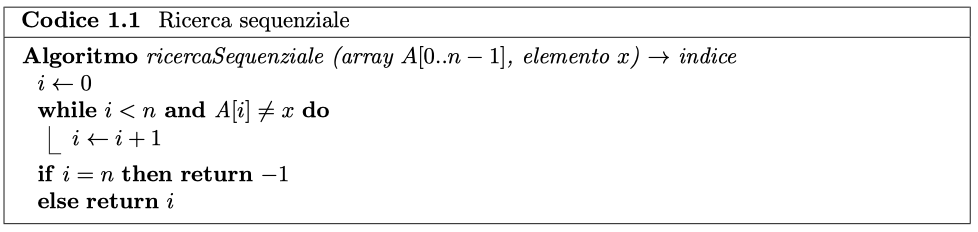
\includegraphics[width=\textwidth]{1-1.png}
    \centering
\end{figure}

\noindent Posso rendere l'algoritmo più "intelligente" cercando a partire dal fondo.
In questo modo se l'elemento non è nell'array l'indice diventa automaticamente -1.
\begin{figure}[h]
    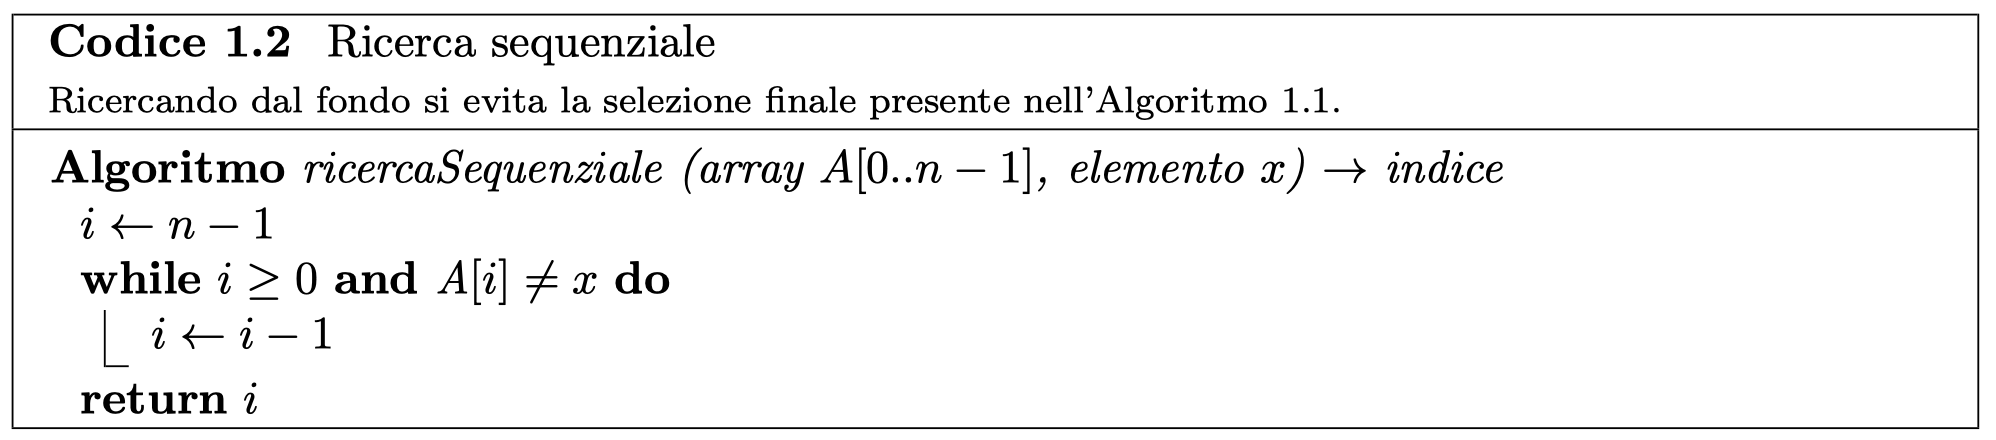
\includegraphics[width=\textwidth]{1-2.png}
    \centering
\end{figure}

\noindent {\textbf{Tempo:}} $\Theta(n)$
\clearpage

\subsection{Ricerca binaria o dicotomica}
Se ho un array ordinato posso usare un algoritmo di ricerca binaria.

\begin{figure}[h]
    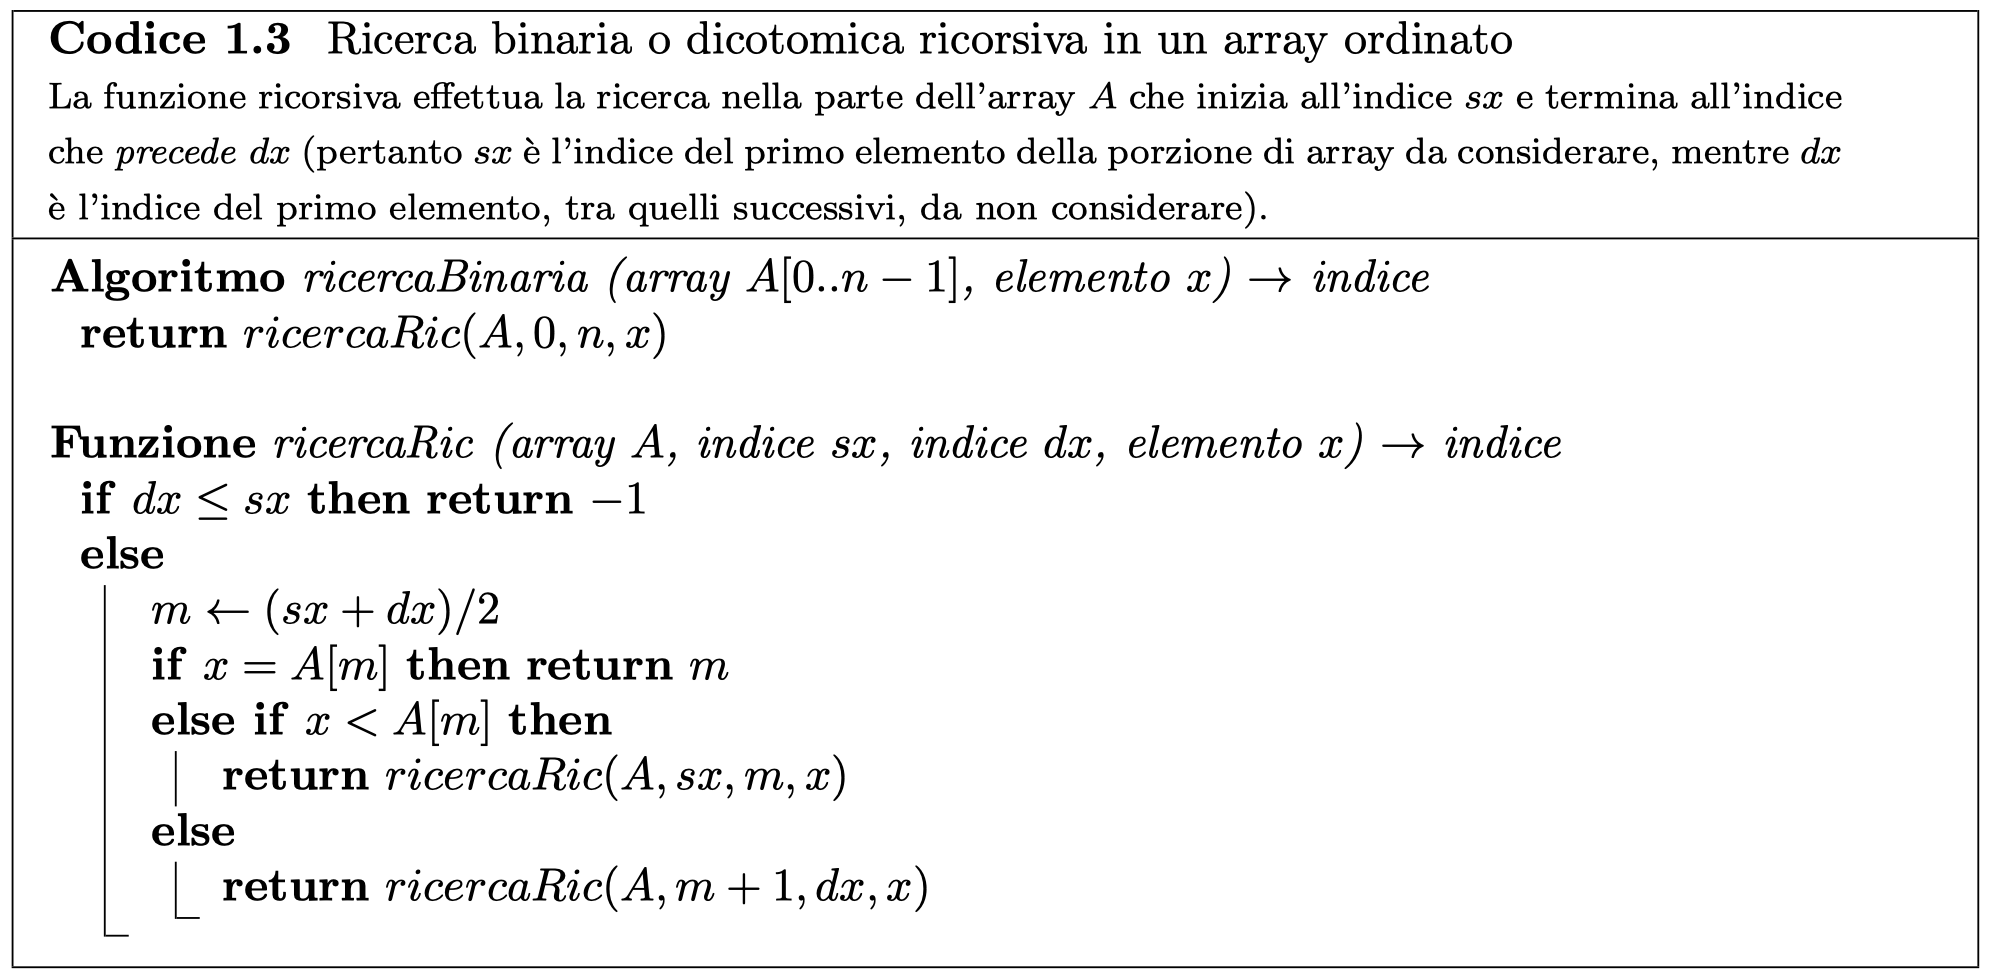
\includegraphics[width=\textwidth]{1-3.png}
    \centering
\end{figure}

\begin{figure}[h]
    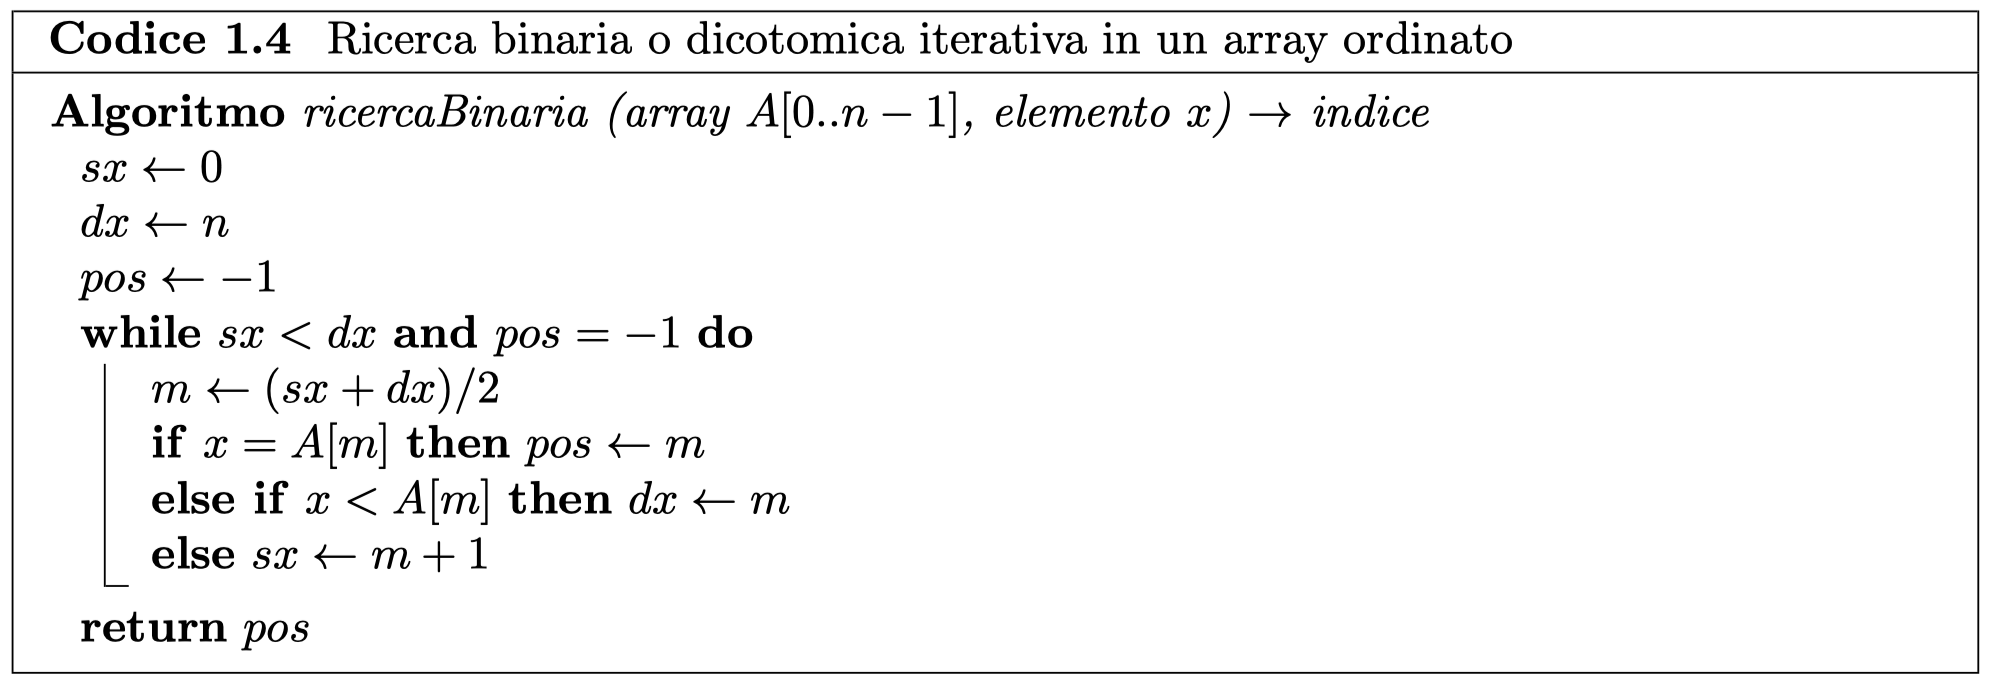
\includegraphics[width=\textwidth]{1-4.png}
    \centering
\end{figure}
\clearpage

\subsubsection{Alcune note sullo pseudocodice}
\begin{itemize}
    \item {\emph{Indici degli array}}\\
    Quando si definisce un array (in questo caso nei parametri degli algoritmi o della funzione), 
    il range di indici viene indicato qualora sia rilevante per la scrittura dell’algoritmo. 
    Quando non sia rilevante o sia chiaro dal contesto, il range viene omesso 
    (come, in questo esempio, per il parametro A della funzione ricercaRic).

    \item {\emph{Operatori logici}}\\
    Assumiamo che per congiunzione ({\emph{and}}) e disgiunzione ({\emph{or}}) sia utilizzata la 
    {\emph{lazy-evaluation}}. Pertanto in una condizione della forma 
    $a$ {\textbf{and}} $b$ la condizione $b$ viene valutata solo se $a$ è vera, 
    mentre in una condizione della forma $a$ {\textbf{or}} $b$ la seconda viene valutata solo se $a$ è falsa.

    \item {\emph{Passaggio di parametri}}\\
    Assumiamo che per i tipi semplici il passaggio di parametro avvenga sempre
    {\emph{per valore}} mentre per i tipi strutturati avvenga il passaggio {\emph{per riferimento}}.

    
\end{itemize}

\clearpage
\section{Algoritmi di ordinamento o sorting}

In questa sezione vediamo alcuni algoritmi che servono per ordinare
vettori di strutture complesse come oggetti o record. Un particolare campo
è scelto come {\textbf{chiave}} per l'ordinamento.
Studieremo principalmente algoritmi di ordinamento basati su confronti
tra chiavi e stimeremo la complessità di questi algoritmi in funzione della 
lunghezza del vettore da ordinare, calcolando prima di tutto il numero di confronti eseguiti.\\
Un algoritmo di ordinamento è detto {\textbf{stabile}} se preserva l'ordine 
relativo tra record con la medesima chiave.
Esistono due tipologie di ordinamento:
\begin{enumerate}
    \item {\emph{Ordinamento interno:}}\\
    I dati da ordinare sono in memoria centrale $\rightarrow$ accesso diretto agli elementi

    \item {\emph{Ordinamento esterno:}}\\
    I dati da ordinare sono in memoria di massa $\rightarrow$ accesso ai blocchi
    di dati con possibile lentezza dovuta dall'hardware dalle periferiche.

\end{enumerate}

\noindent Vedremo principalmente tecniche di ordinamento interno, tra cui troviamo tecniche
\begin{enumerate}
    \item {\textbf{Elementari}}\\
    Utilizzano nel caso peggiore un numero quadratico di confronti
    \begin{itemize}
        \item Per selezione ({\emph{SelectionSort}})
        \item Per inserimento ({\emph{InsertionSort}})
        \item A bolle ({\emph{BubbleSort}})
    \end{itemize}

    \item {\textbf{Avanzate}}\\
    Utilizzano un numero di confronti dell'ordine di $n \log n$ (tranne {\emph{QuickSort}}, il cui
    caso peggiore risulta però molto raro)
    \begin{itemize}
        \item Per fusione ({\emph{MergeSort}})
        \item Veloce ({\emph{QuickSort}})
        \item Basato su heap ({\emph{HeapSort}})
    \end{itemize}
\end{enumerate}
\clearpage



\section{Selection Sort}
\begin{enumerate}
    \item Prima del passo principale $k$, con $k = 0,\dots, n - 1$, i primi 
    $k$ elementi dell'array sono al loro posto definitivo, cioè sono ordinati
    tra loro e sono minori o uguali degli elementi successivi

    \item Si seleziona l'elemento che andrà collocato in posizione $k$, cioè
    il minimo della parte non ordinata (quindi il minimo tra $A[k],\dots,A[n-1]$)

    \item Lo si colloca in posizione $k$, scambiandolo con l'elemento ivi presente
    \item In questo modo, dopo il passo principale $k$, i primi $k$ elementi
    risultano collocati nella loro posizione definitiva.
\end{enumerate}

\noindent Dopo il passo $n - 2$ la parte non ordinata contiene solo un elemento e, in base
al punto 1, questo è maggiore o uguale dei precedenti, e dunque si trova nella sua
posizione definitiva. Pertanto non è necessario eseguire il passo $n - 1$

\begin{figure}[h]
    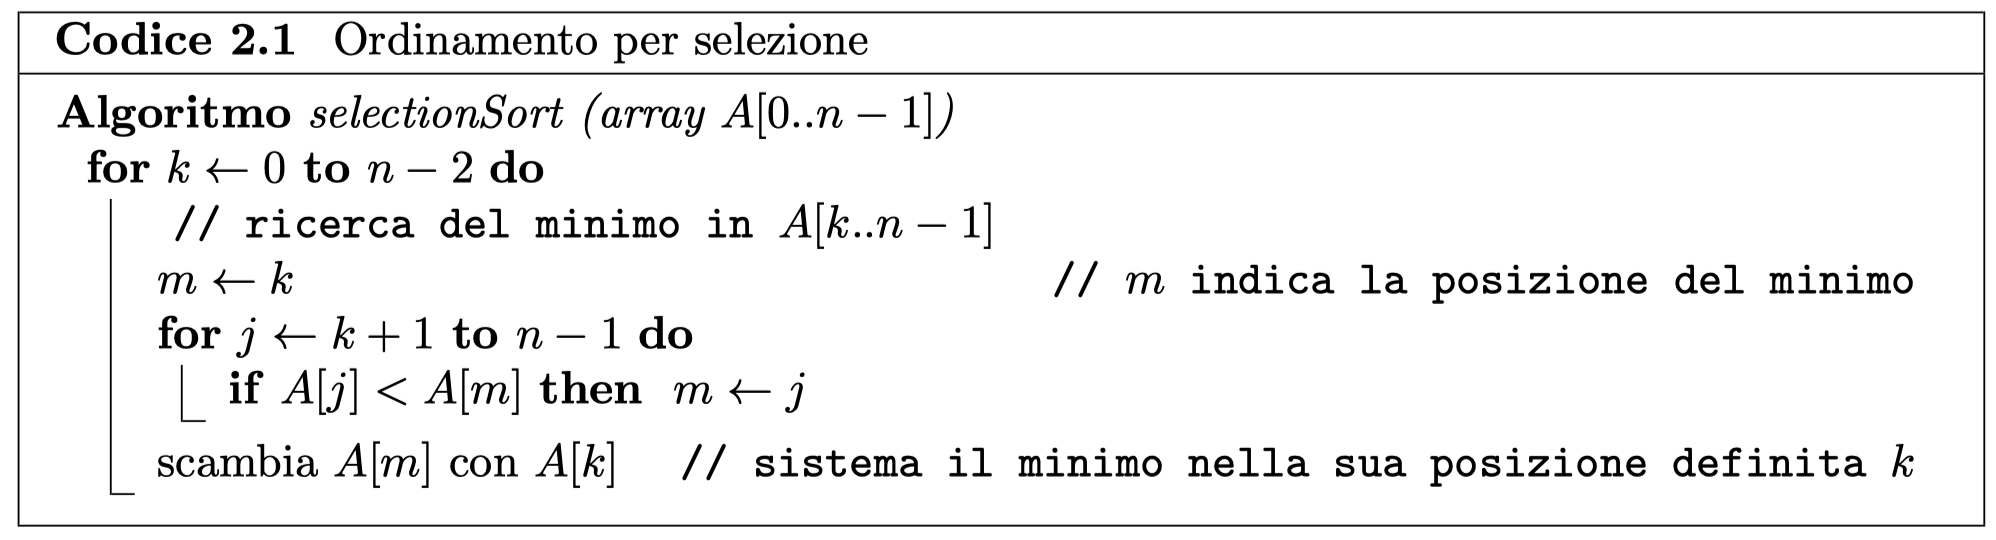
\includegraphics[width=\textwidth]{selectionsort.png}
    \centering
\end{figure}

\subsubsection*{Numero di confronti}
Nell'iterazione $k$ del ciclo principale viene ricercato il minimo della porzione di 
vettore da posizione $k$ a posizione $n - 1$, effettuando quindi $n-k-1$ confronti.
Sommando su tutte le iterazioni $k$ del ciclo principale otteniamo il numero totale
di confronti $\frac{n(n-1)}{2} = \Theta(n^2)$, che vengono eseguiti sempre indipendentemente dal
contenuto dell'array.

\subsubsection*{Spazio}
L'algoritmo, oltre all'array da ordinare, utilizza un numero costante di variabili.
Pertanto la quantità di spazio aggiuntivo è costante.
\clearpage
\section{Insertion Sort}
\begin{enumerate}
    \item Si memorizza l'elemento $A[k]$ da sistemare in una variabile $x$
    \item Si ispeziona la porzione di array $A[0..k-1]$ {\emph{da destra verso sinistra}},
    spostando avanti di una posizione ogni elemento maggiore di $x$, in modo da "fare posto"
    all'elemento da inserire
    \item Individuata la posizione in cui inserire $x$ (quindi quando si 
    raggiunge un elemento che non è maggiore di $x$ o quando si è ispezionata
    tutta la porzione iniziale di array), si inserisce $x$ (gli elementi successivi sono già stati 
    spostati durante il passo 3)
\end{enumerate}

\begin{figure}[h]
    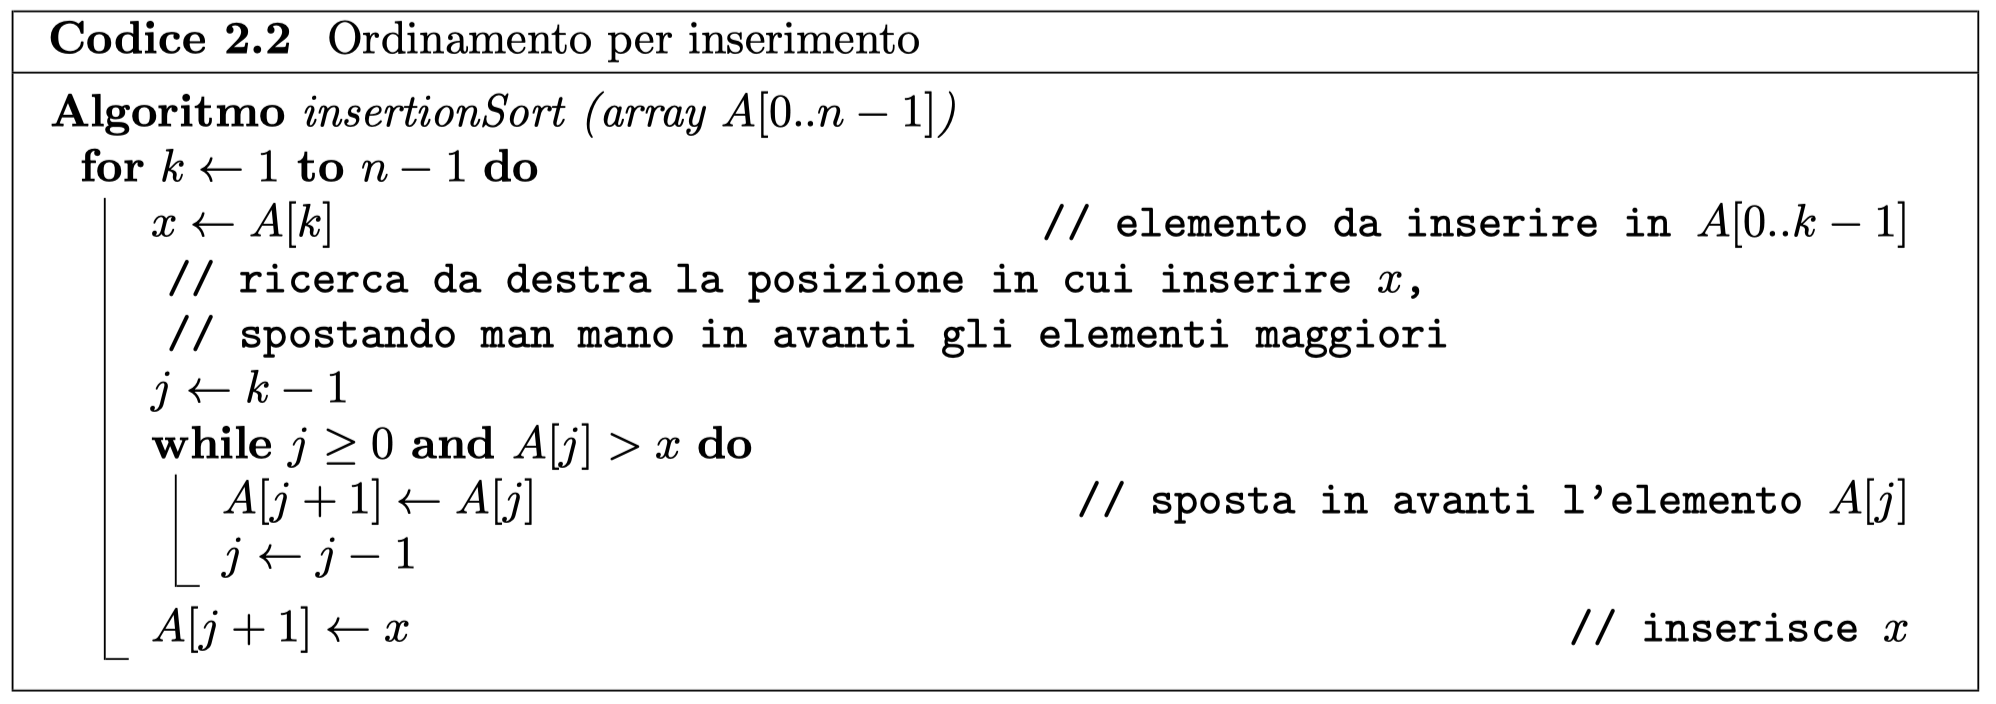
\includegraphics[width=\textwidth]{insertionsort.png}
\end{figure}

\subsubsection*{Numero di confronti}
Nel caso peggiore ogni elemento dell'array viene confrontato con ogni altro
elemento dell'array. Pertanto vengono effettuati $\frac{n(n-1)}{2} = \Theta(n^2)$
confronti. Il caso peggiore si verifica nel caso in cui l'array sia ordinato al 
contrario, mentre nel caso migliore, ovvero quello in cui l'array è già ordinato,
vengono effettuati $n - 1$ confronti.

\subsubsection*{Spazio}
L'algoritmo, oltre all'array da ordinare, utilizza un numero costante di variabili.
Pertanto la quantità di spazio aggiuntivo è costante.
\clearpage
\section{Bubble Sort}
L'idea di base è quella di scandire ripetutamente l'array dal primo all'ultimo
elemento scambiando tra loro gli elementi adiacenti che non risultino ordinati.
L'array sarà ordinato quando si riuscirà ad effettuare una scansione senza alcuno
scambio.

\begin{figure}[h]
    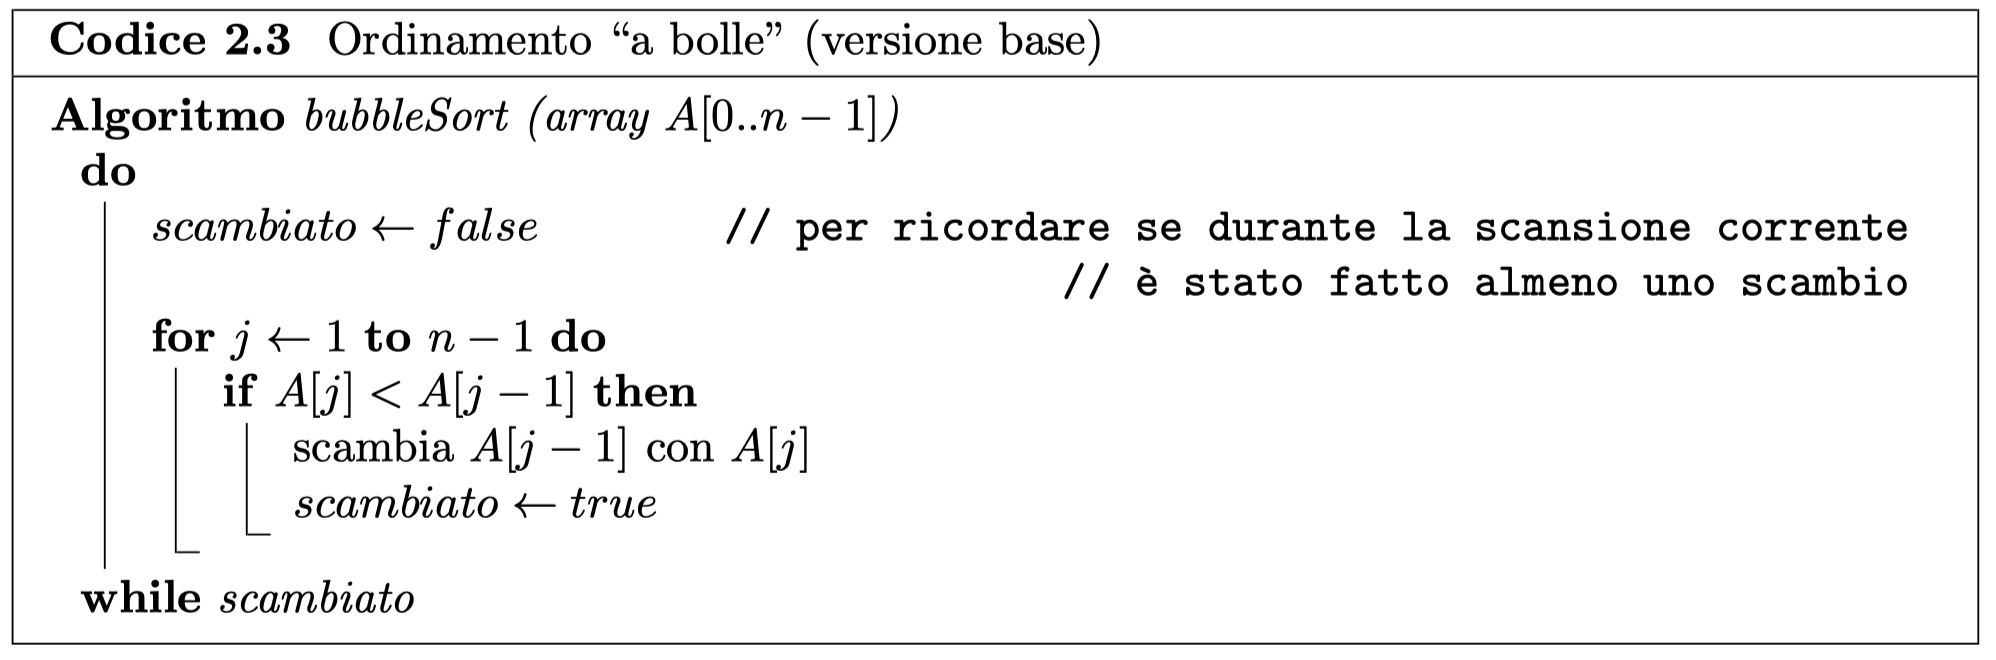
\includegraphics[width=\textwidth]{bubblesortbase.png}
\end{figure}

\subsubsection*{Esempio di esecuzione versione base}

\begin{figure}[h]
    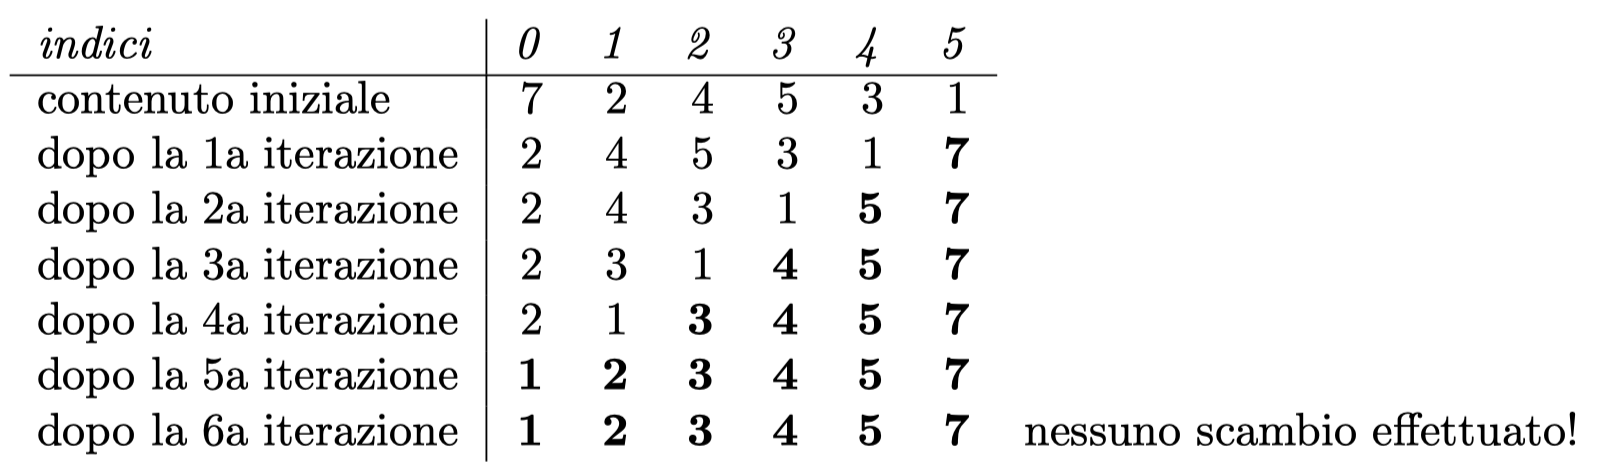
\includegraphics[width=\textwidth]{bubblesortexbase.png}
\end{figure}

\noindent Dopo la $i$-esima iterazione, gli ultimi $i$ elementi dell'array sono 
al loro posto definitivo e dunque non è più necessario esaminarli. Per la 
stessa ragione dopo $n - 1$ scansioni, gli $n - 1$ elementi più grandi hanno 
raggiunto la loro posizione e di conseguenza l'elemento più piccolo deve trovarsi
nell'unica posizione che resta, ovvero quella di indice 0. Pertanto, dopo
aver effettuato $n - 1$ iterazioni l'algoritmo si può fermare anche se 
nell'ultima scansione ci sono stati scambi. Possiamo quindi scrivere una versione migliorata 
dell'algoritmo.
\clearpage

\subsubsection*{Versione migliorata}
\begin{figure}[h]
    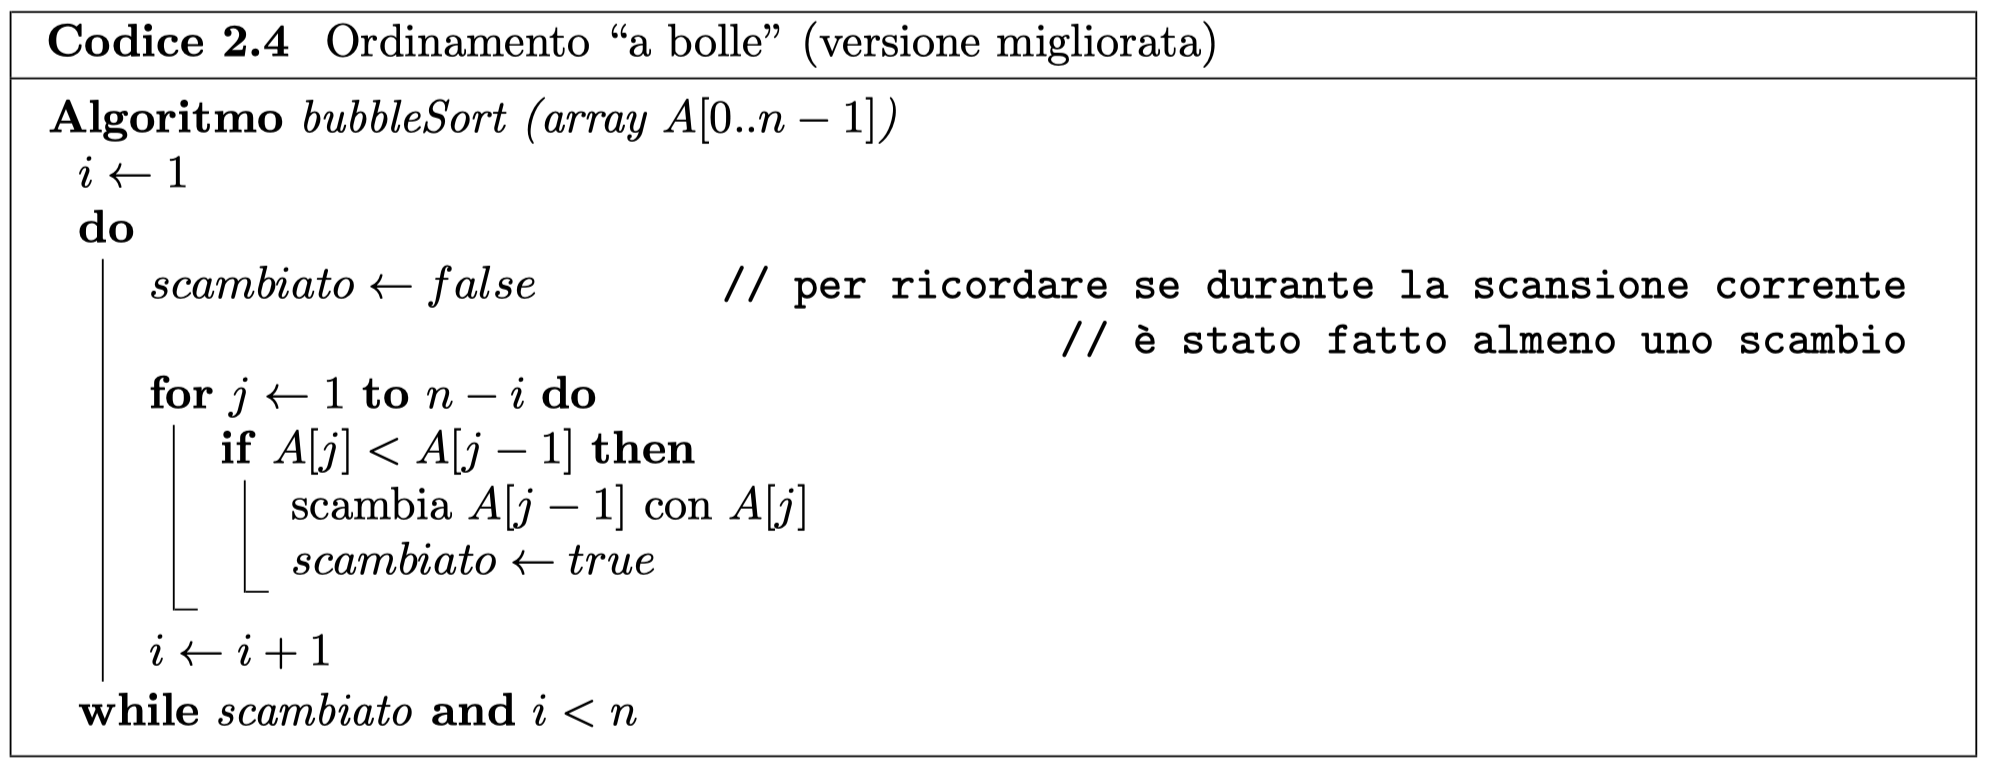
\includegraphics[width=\textwidth]{bubblesortmigliorato.png}
\end{figure}

\subsubsection*{Esempio di esecuzione versione migliorata}
\begin{figure}[h]
        
\includegraphics[width=\textwidth]{bubblesortexmigliorato.png}
\end{figure}

\subsubsection*{Numero di confronti}
Nell'iterazione $i$ del ciclo principale si effettuano esattamente $n - 1$ confronti.
Il ciclo principale viene eseguito a partire da $i = 1$, incrementando fino al più
a $n - 1$. Pertanto sommando su tutte le iterazioni il numero di confronti è al massimo $\frac{n(n-1)}{2} = \Theta(n^2)$
nel caso peggiore, che si ha quando l'array è ordinato al contrario.
Se invece l'array è già ordinato il numero di confronti è $n - 1$ 

\subsubsection*{Spazio}
L'algoritmo, oltre all'array da ordinare, utilizza un numero costante di variabili.
Pertanto la quantità di spazio aggiuntivo è costante.
\clearpage

\subsection{Una considerazione su confronti e spostamenti}
Abbiamo detto che la stima del tempo di calcolo di questi algoritmi 
può avvenire a partire da quella del numero di confronti, 
moltiplicando il numero di confronti per il tempo necessario per 
effettuare ciascun confronto. Questo è vero a patto che i confronti tra chiavi 
siano le operazioni più costose effettuate dagli algoritmi. 
Potremmo calcolare anche il numero di spostamenti di elementi. 
Da questo calcolo possiamo scoprire che tra i tre algoritmi presentati sopra, l’ordinamento per selezione
è quello che effettua un numero di spostamenti più basso. 
Ma quanto costano gli spostamenti in termini di tempo? Come per i confronti, 
se stiamo ordinando numeri interi di grandezza fissata, come i valori dei tipi {\texttt{int}} e {\texttt{long}}, 
gli spostamenti sono effettuati mediante assegnamenti che copiano un numero fissato di bit, e quindi avvengono in tempo costante. 
Se tuttavia, come avviene nella pratica, stiamo ordinando rispetto a un campo chiave dei record di grandi dimensioni, 
la copia di interi record diventa costosa in termini di tempo e il numero di spostamenti può essere un parametro critico, 
anche più importante del numero di confronti, per valutare il tempo impiegato da un algoritmo.
Questo problema può essere evitato utilizzando i puntatori: 
anzichè memorizzare negli elementi dell’array i record da ordinare, 
possiamo memorizzare i puntatori ad essi. 
Quindi, ogni cella dell’array conterrà il puntatore a un record, memorizzato altrove. 
In questo modo, per effettuare uno spostamento, non è necessario copiare l’intero record, 
ma solo copiare dei puntatori ai record. La dimensione dei puntatori può essere considerata costante 
(dipende dalla grandezza delle memoria che può essere indirizzata).
\clearpage
\section{Merge Sort}
L'algoritmo di ordinamento per fusione si basa sul seguente schema:
\begin{itemize}
    \item Un array di un solo elemento è già ordinato (\emph{caso base})
    \item Per ordinare un array $A$ contenente $n > 1$ elementi possiamo:
    \begin{enumerate}
        \item suddividere $A$ in due array $B$ e $C$ di $n/2$ elementi ciascuno,
        corrispondenti alla prima e alla seconda metà dell'array $A$ (Nel caso $n$ 
        sia dispari le due metà saranno di $\lfloor n/2 \rfloor$ e $\lceil n/2 \rceil$ )
        \item ordinare separatamente gli array
        \item "fondere" gli array ordinati $B$ e $C$ nell'array $A$, in modo da
        ottenere un array ordinato contenente gli elementi di $B$ e $C$.
    \end{enumerate}
\end{itemize}

\noindent L'operazione di fusione ({\texttt{merge}}) di due array ordinati
in un array ordinato è più semplice rispetto all'ordinamento di un array.

\noindent Studiamo come effettuare il merge. Disponiamo di due vettori $B$ e $C$ ordinati
in modo non decrescente, e vogliamo ottenere un vettore $X$ ordinato che contenga
gli stessi elementi di $B$ e $C$.

\begin{enumerate}
    \item Creiamo un vettore $X$ la cui lunghezza sia la somma delle lunghezze di 
    $B$ e $C$
    \item Ispezioniamo $B$ e $C$ iniziando a considerare gli elementi minimi, ovvero quelli
    nella prima posizione dei due vettori
    \item Confrontiamo i due elementi e scegliamo il minimo, copiandolo nella 
    prima posizione libera di $X$. Inoltre, nel vettore da cui abbiamo preso
    l'elemento, possiamo considerare quello di posizione successiva.
    \item Ripetiamo le operazioni precedenti fino a raggiungere la fine di uno dei due array
    \item Copiamo in $X$ tutti gli elementi rimanenti dell'altro array
\end{enumerate}

\subsubsection*{Numero di confronti}
Indicando con $C(n)$ il numero di confronti effettuato da {\texttt{mergeSort}}
possiamo scrivere la seguente equazione di ricorrenza.

\begin{equation*}
    C(n)=\begin{cases}
        C(\lfloor n/2 \rfloor) + C(\lceil n/2 \rceil) + C_{\texttt{merge}}(n) & \text{se $n > 1$}\\
        0 & \text{altrimenti}
    \end{cases}
\end{equation*}

Nel caso peggiore $C_{\texttt{merge}}(n) = n - 1$. Risolvendo per sostituzione
otteniamo $C(n) = \Theta(n \log n)$

\subsubsection*{Tempo di calcolo}
Ci sono varie operazioni costose sia in termini di tempo che in termini di spazio:
dobbiamo creare due array $B$ e $C$, copiarvi gli elementi di $A$ e, dopo il 
merge, ricopiare tutti gli elementi nell'array iniziale. Indicando con $T(n)$ il tempo
utilizzato dall'algoritmo per ordinare un array di lunghezza $n$ osserviamo che:
\begin{itemize}
    \item Se l'array contiene al più 1 elemento, l'algoritmo usa tempo costante.
    Indichiamo tale tempo con $a$
    \item Se l'array contiene $n > 1$ elementi, allora $T(n)$ è la somma dei seguenti tempi:
    \begin{itemize}
        \item Tempo per la creazione dei due array: $\Theta(n)$
        \item Tempo per ordinare i due array: $T(\lfloor n/2 \rfloor) + T(\lceil n/2 \rceil)$
        \item Tempo per il merge: $\Theta(n)$
    \end{itemize}

\end{itemize}
\noindent Possiamo quindi scrivere l'equazione di ricorrenza
\begin{equation*}
    T(n)=\begin{cases}
        2T(n/2) + bn + c & \text{se $n > 1$}\\
        a & \text{altrimenti}
    \end{cases}
\end{equation*}
dove $b$ e $c$ sono due costanti.\\
Risolvendo per sostituzione ottengo $T(n) = \Theta(n \log n)$

\subsubsection*{Implementazione}
Come abbiamo visto, l'implementazione di una versione base di {\texttt{mergeSort}}
richiede l'uso di tempo e spazio per gli array $B$ e $C$. Possiamo implementare
l'algoritmo in maniera differente, servendoci direttamente dell'array $A$ da ordinare
e di due indici che delimitano la parte da ordinare.
Al contrario, per effettuare la procedura {\texttt{merge}} ci serviremo di un 
array ausiliario, che per evitare sprechi verrà creato preliminarmente
e verrà usato da tutte le chiamate di {\texttt{merge}}.
La precedente analisi relativa al numero di confronti non cambia e il tempo
rimane dell'ordine di $n \log n$.

\begin{figure}[h]
    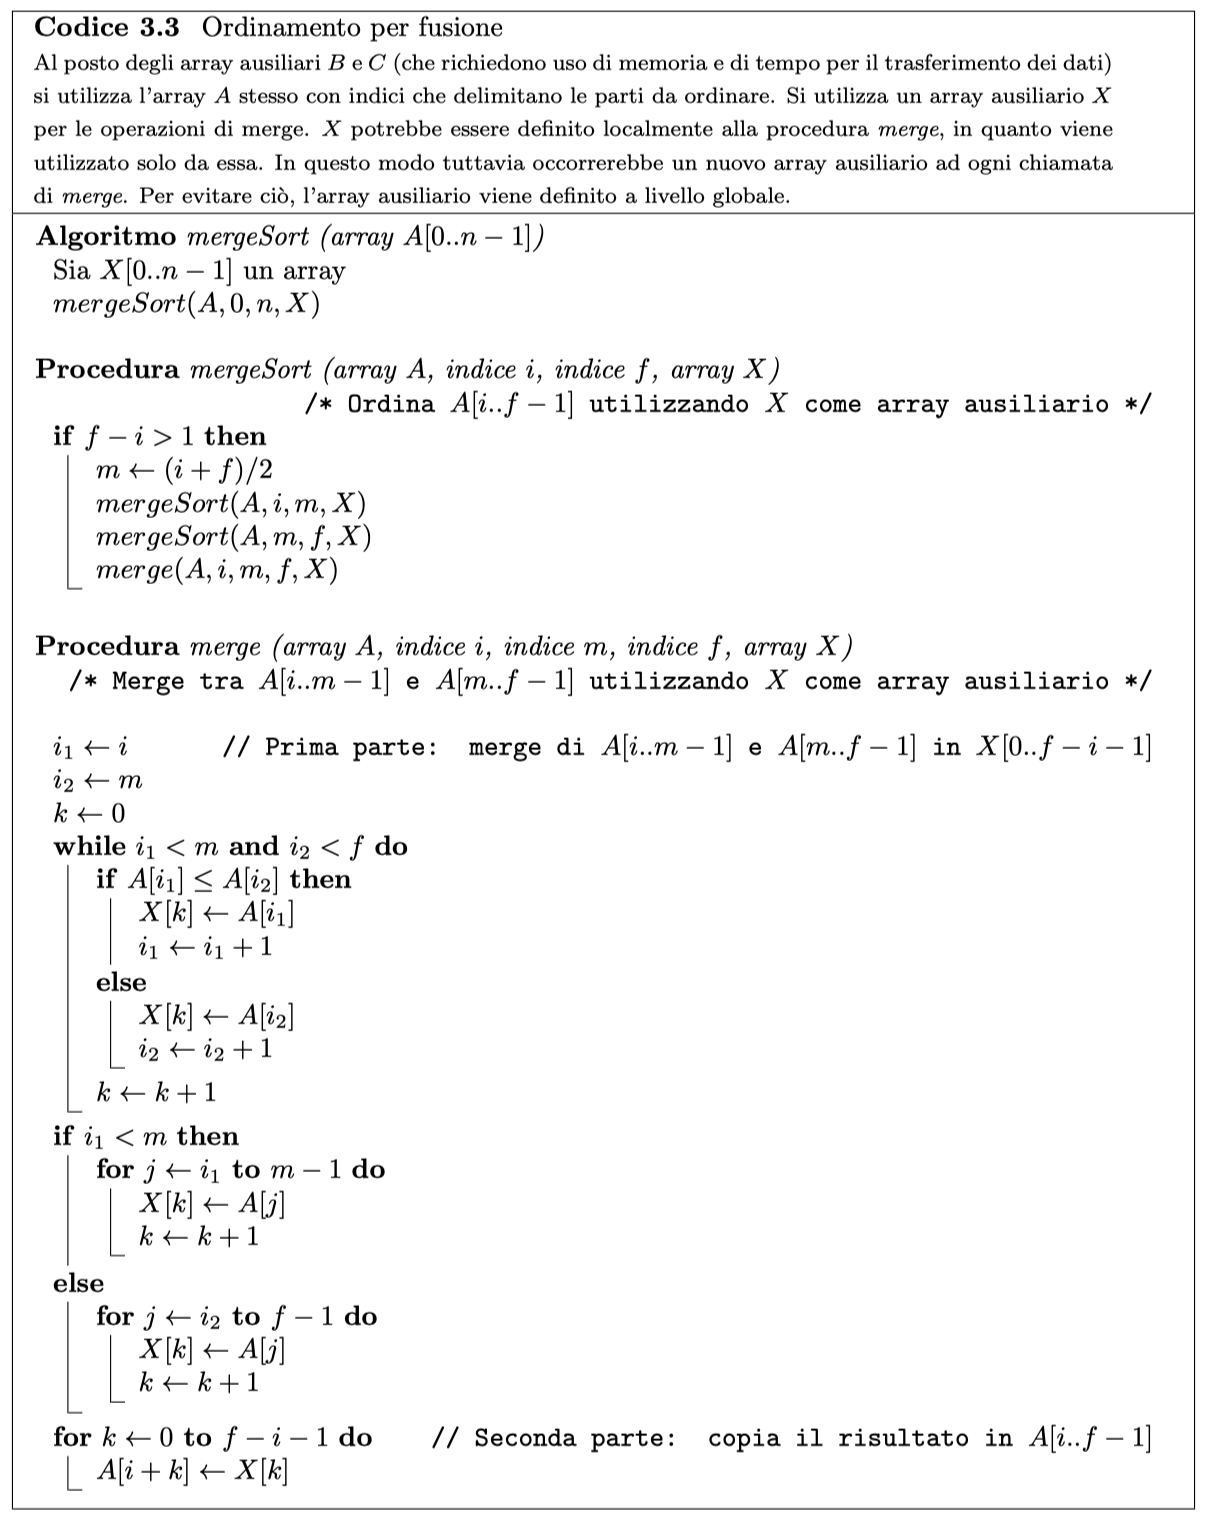
\includegraphics[width=\textwidth]{mergesort.png}
\end{figure}

\clearpage

\subsubsection*{Spazio}
L'algoritmo non è in loco, in quanto utilizza un array ausiliario per effettuare
il merge. L'array è di $n$ elementi, quindi usa spazio $\Theta(n)$.
Dobbiamo inoltre considerare lo spazio utilizzato dallo stack per gestire la ricorsione.
In ciascun record di attivazione di {\texttt{mergeSort}} devono essere memorizzati
gli indici $i$ ed $f$ che servono a delimitare la porzione di array da delimitare e la 
variabile $m$. Pertanto la dimensione di ogni record è costante. Per calcolare l'altezza
dello stack utilizziamo un'equazione di ricorrenza.
\begin{itemize}
    \item Se $n \le 1$ (caso base) non viene effettuata alcuna chiamata ricorsiva.
    Pertanto viene utilizzato solo il record di attivazione corrente e $H(n) = 1$
    \item Se $n > 1$ viene effettuata una prima chiamata ricorsiva su un array di 
    lunghezza $\lfloor n/2 \rfloor$, che dunque utilizzerà altezza $H(\lfloor n/2 \rfloor)$.
    terminata tale chiamata si effettua una seconda chiamata sull'altra parte di array,
    quindi con altezza $H(\lceil n/2 \rceil)$. Poichè al termine di ciascuna
    chiamata ricorsiva lo stack viene riportato all'altezza che aveva prima della chiamata,
    la parte di stack utilizzata dalla prima chiamata viene riutilizzata per la seconda.
    Pertanto l'altezza dello stack utilizzata dalle due chiamate è il massimo tra 
    $H(\lfloor n/2 \rfloor)$ e $H(\lceil n/2 \rceil)$.
\end{itemize}

\noindent Otteniamo dunque 
\begin{equation*}
    H(n) = \begin{cases}
        max(H(\lfloor n/2 \rfloor), H(\lceil n/2 \rceil)) + 1 & \text{se $n > 1$}\\
        1 & \text{altrimenti}
    \end{cases}
\end{equation*}

Questo ci permette di concludere che l'altezza dello stack è logaritmica rispetto a n, 
ed è in particolare $\Theta(\log n)$.
\clearpage

\section{Quick Sort}
Supponiamo di dover ordinare la sequenza di numeri\\[12pt]
{\texttt{44 55 12 42 94 6 18 67}}\\[12pt]
Scegliamo all'interno di essa un qualunque elemento, ad esempio {\texttt{42}}
(che chiameremo {\emph{perno}} o {\emph{pivot}}), e costruiamo due sequenze nelle quali collochiamo
rispettivamente tutti gli elementi minori o uguali al perno e tutti quelli maggiori, in qualunque ordine:\\[12pt]
{\texttt{12 42 6 18 $\quad$ 44 55 94 67}}\\[12pt]
Ordinando separatamente le due sequenze e concatenandole otteniamo la 
sequenza ordinata:\\[12pt]
{\texttt{6 12 18 42 44 55 67 94}}\\[12pt]

\begin{figure}[h]
    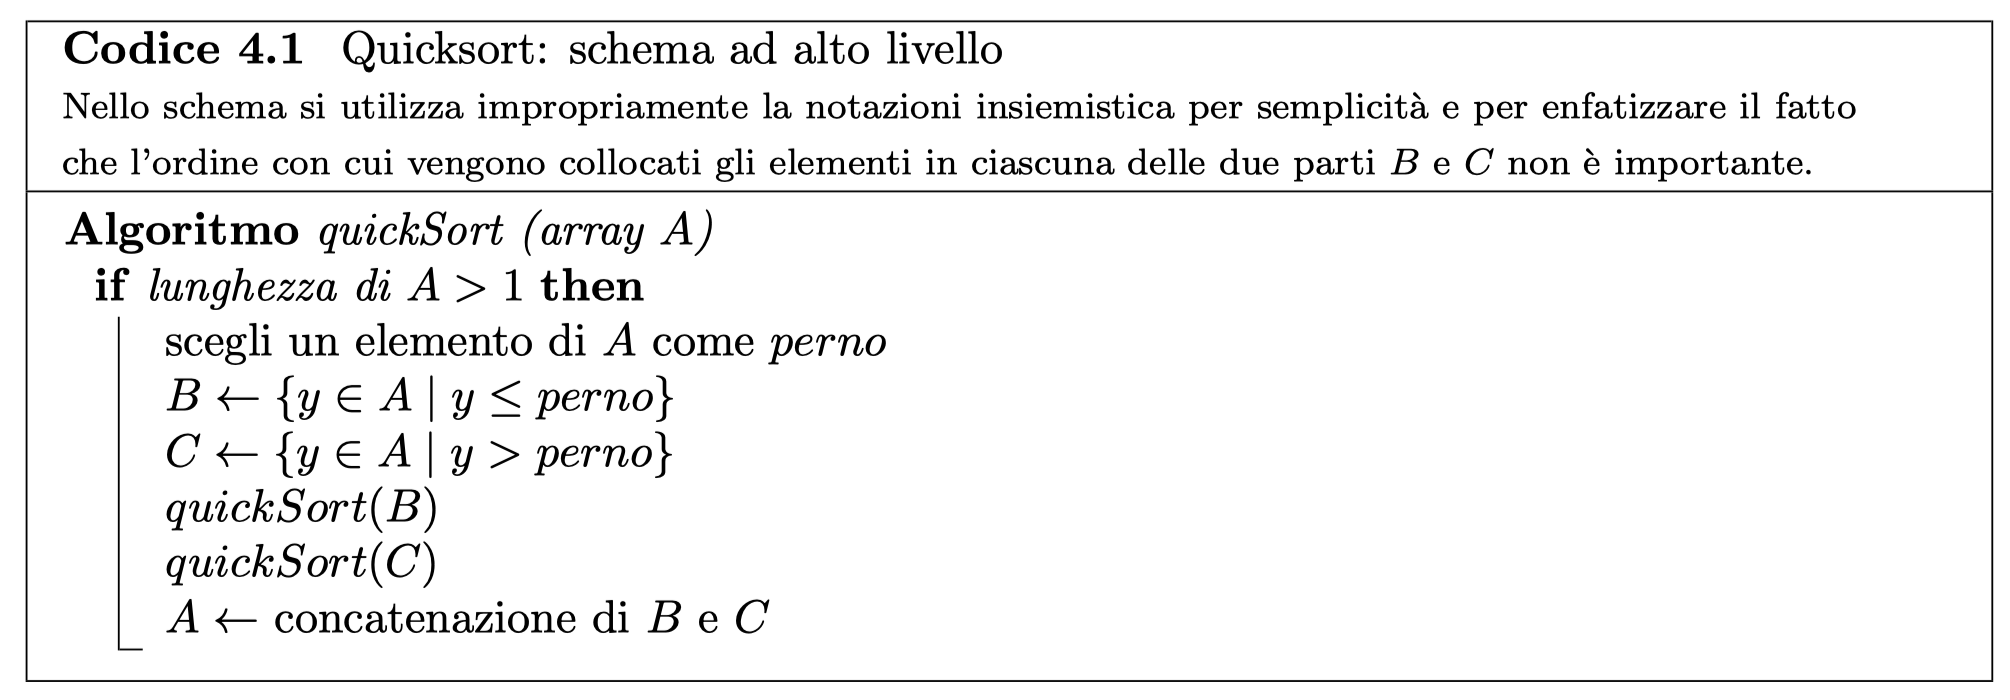
\includegraphics[width=\textwidth]{quicksortal.png}
\end{figure}

\subsection{Partiziona}

Per creare la partizione dell'array procediamo nel seguente modo:
\begin{enumerate}
    \item Scegliamo come perno l'elemento più a sinistra dell'array
    \item Scansioniamo l'array da destra verso sinistra fino al primo elemento minore o uguale al perno
    \item Scansioniamo l'array da sinistra verso destra fino al primo elemento maggiore del perno
    \item Se le due scansioni non si sono incontrate, scambiamo i due elementi individuati e proseguiamo le scansioni ai passi 2 e 3
    \item Quando ogni elemento è stato confrontato con il perno, scambiamo il perno con l'elemento su cui si è arrestata la scansione da destra 
\end{enumerate}

\noindent
Per le scansioni da destra e da sinistra utilizziamo due indici di nome 
$dx$ e $sx$, che indicano gli elementi correntemente ispezionati dalle due scansioni.
Ad ogni passo tutti gli elementi a sinistra dell'indice $sx$ risultano minori 
o uguali al perno, mentre quelli a destra di $dx$ maggiori del perno. Quando i due indici
si incontrano o $sx \ge dx$ tutti gli elementi sono stati ispezionati.
Inoltre, l'elemento di indice $dx$ è minore o uguale al perno. A questo punto
è sufficiente scambiare questo elemento con il perno per ottenere la partizione.

\begin{figure}[h]
    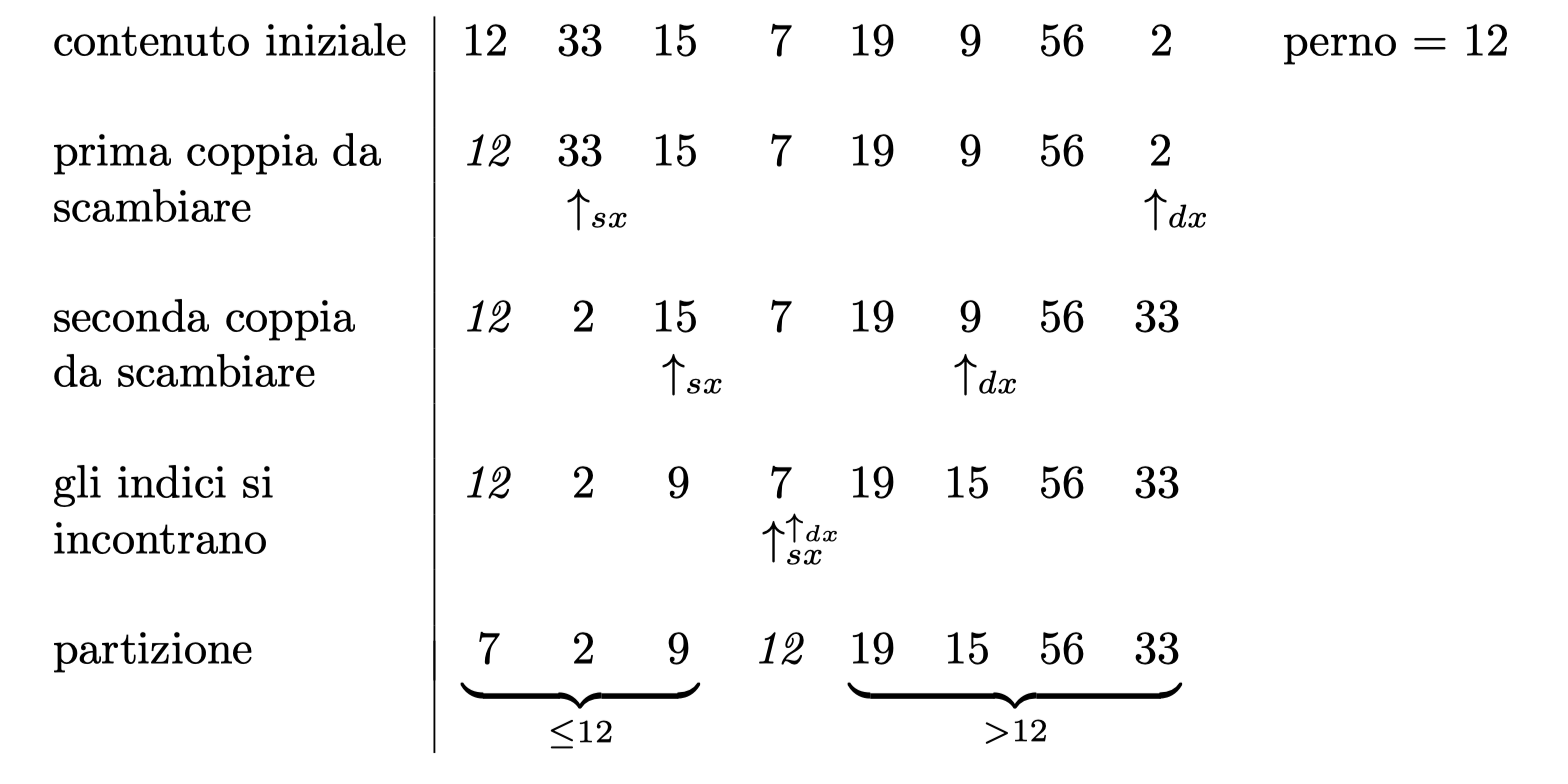
\includegraphics[width=\textwidth]{espartizione.png}
\end{figure}

\begin{figure}[h]
    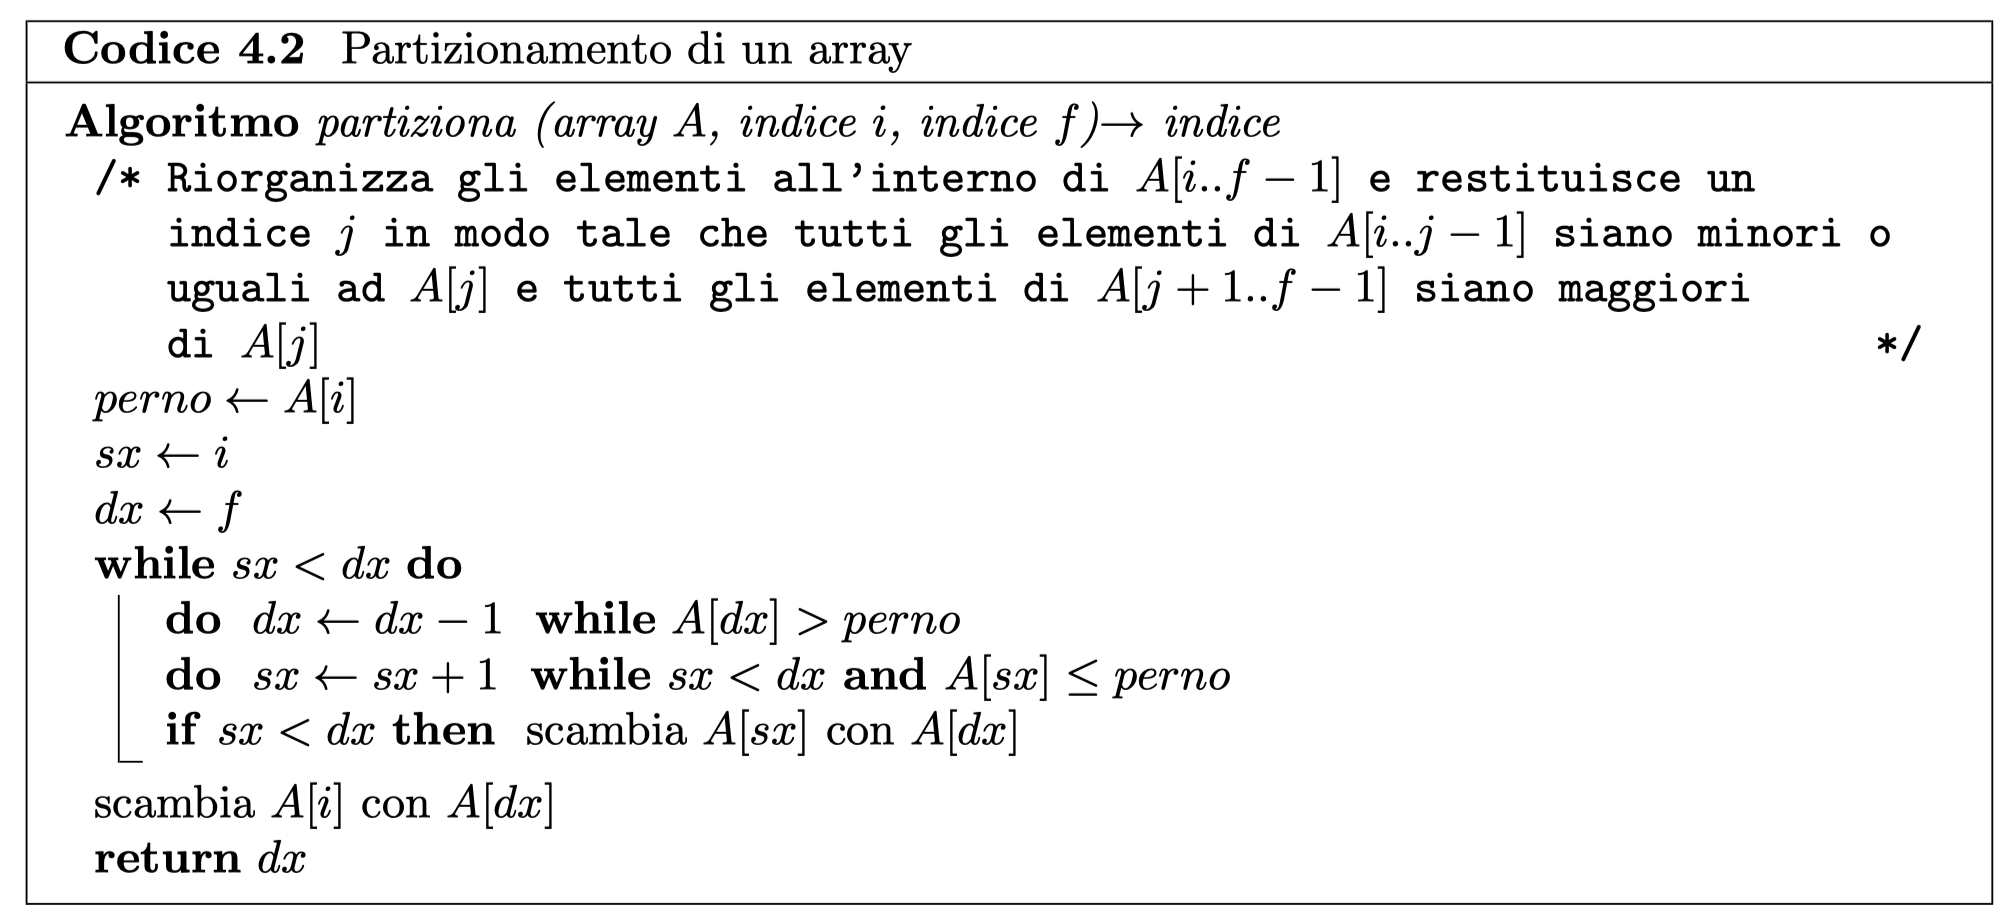
\includegraphics[width=\textwidth]{partiziona.png}
\end{figure}
\clearpage

\subsection*{Numero di confronti}

\begin{figure}[h]
    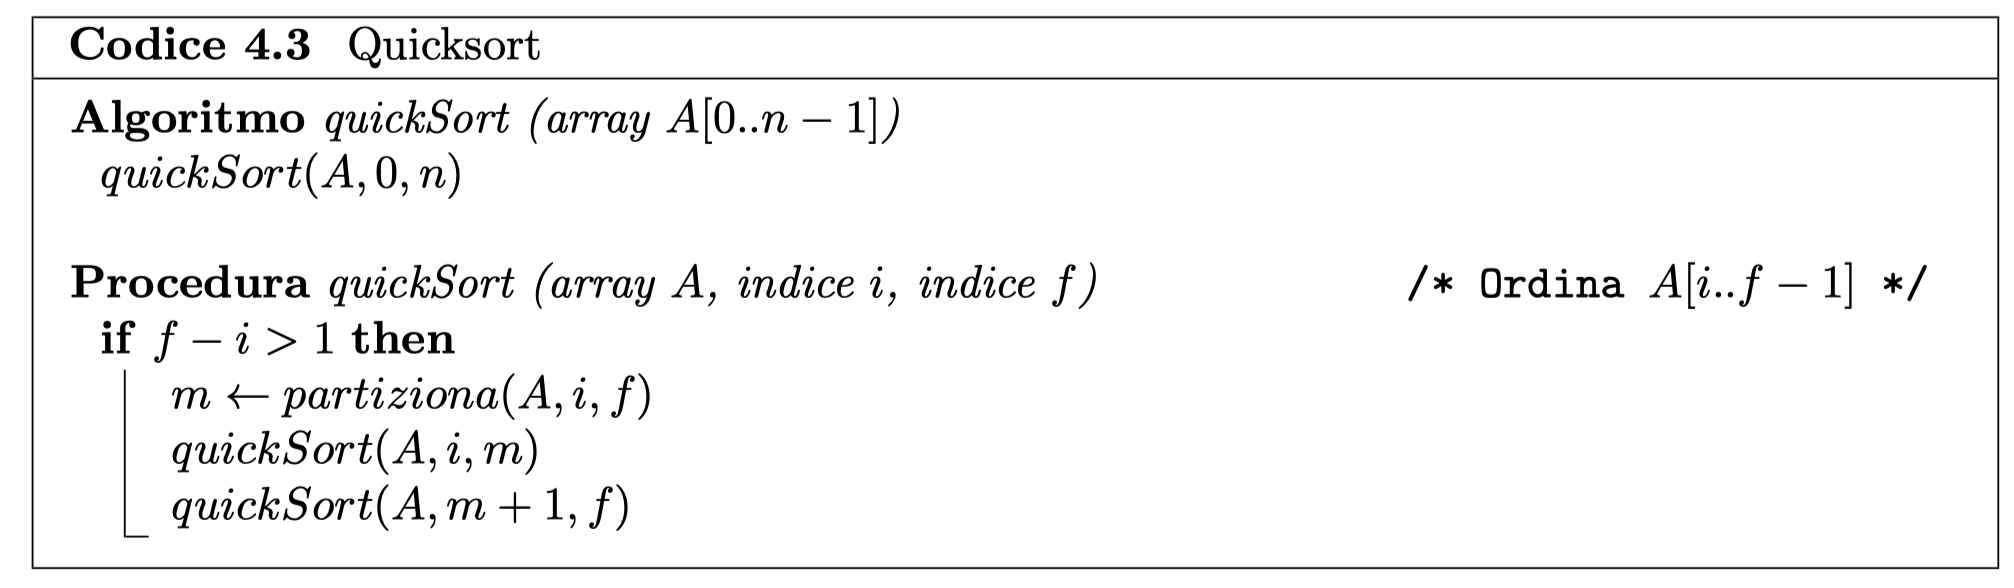
\includegraphics[width=\textwidth]{quicksort.png}
\end{figure}

Per effettuare la partizione ogni elemento dell'array deve essere confrontato con il perno
(eccetto il perno stesso). Pertanto vi sono almeno $n - 1$ confronti. Per semplicità di calcolo
utilizzeremo solo $n$\\

\subsubsection*{Caso peggiore}
Nel caso peggiore $C_{w}(n)$ {\texttt{quickSort}} esegue il seguente numero di confronti:
\begin{equation*}
    C_{w}(n) = \begin{cases}
        n + max{C_{w}(n) + C_{w}(n-k-1) | 0 \le k \le n} & \text{se $n > 1$}\\
        0 & \text{altrimenti}
    \end{cases}
\end{equation*}
Il secondo addendo della somma rappresenta il numero di confronti nelle chiamate 
ricorsive nell'ipotesi che, dopo la partizione, vi siano $k$ elementi a sinistra
del perno e $n-k-1$ a destra. Dato che stiamo studiando il caso peggiore 
consideriamo il valore di $k$ che massimizza la somma. Svolgendo i calcoli otteniamo
$C_{w}(n) = \Theta(n^2)$. Pertanto nel caso peggiore (molto raro) {\texttt{quickSort}}
effettua lo stesso numero di confronti degli algoritmi elementari che abbiamo studiato.

\subsubsection*{Caso migliore}
Abbiamo visto che il caso peggiore si ottiene quando ad ogni livello della ricorsione
la partizione risulta sbilanciata. Se, al contrario, l'array viene sempre suddiviso
in due parti circa della stessa lunghezza, il numero di confronti diminuisce drasticamente.
\begin{equation*}
    C_{b}(n) = \begin{cases}
        n + 2C_{b}(n/2) & \text{se $n > 1$}\\
        0 & \text{altrimenti}
    \end{cases}
\end{equation*}

\noindent Svolgendo i calcoli otteniamo $C_{b}(n) = n \log_2 n$

\subsubsection*{Caso medio}
Il numero di confronti effettuato da {\texttt{quickSort}} dipende dalla distribuzione
dei valori all'interno dell'array. Si può calcolare che il caso medio $C(n) \le 1.39n \log_2 n$, 
molto vicino al caso migliore e a {\texttt{mergeSort}}, motivo per cui {\texttt{quickSort}}
viene utilizzato molto spesso. 

\subsubsection*{Spazio di lavoro}
L'algoritmo è in loco ma utilizza spazio aggiuntivo per la ricorsione. Ogni 
record di attivazione deve contenere i parametri $i$ ed $f$ che delimitano
la parte di array da ordinare, oltre alla variabile $m$. Dunque la grandezza
di ciascun record di attivazione è costante. La quantità di memoria utilizzata 
è proporzionale all'altezza raggiunta dallo stack, che nel caso peggiore è $n$.
Si può modificare
l'algoritmo in modo che l'altezza dello stack sia sempre $O(\log n)$ eliminando una chiamata
ricorsiva e ordinando prima la parte destra dell'array e poi la sinistra.

\subsubsection*{Alcune osservazioni}
Possiamo osservare che le prestazioni di {\texttt{quickSort}}, su uno stesso array
possono variare notevolmente in base alla strategia utilizzata per scegliere il perno.
Spesso, per evitare il caso peggiore (array già ordinato), si utilizzano strategie
"randomizzate". Una possibilità è quella di disordinare in modo casuale gli
elementi dell'array prima di eseguire l'algoritmo, un'altra può essere
scegliere un elemento casuale dell'array da usare come perno e scambiarlo con il 
primo elemento, applicando poi la strategia di partizione che abbiamo visto.
Si può osservare che questo metodo di ordinamento non è stabile. 
\clearpage
\section{Strutture dati}
Le strutture dati consistono in una specifica organizzazione delle informazioni,
che permette di realizzare ed implementare un determinato tipo di dati.
La scelta della corretta struttura dati dipende dall'utilizzo che bisogna fare 
dei dati.

Il tipo di una variabile stabilisce i valori e le operazioni che possono essere
eseguite. In generale quando parliamo del tipo non parliamo della rappresentazione
del dato ma del "cosa". La rappresentazione influisce però sull'efficienza delle
operazioni.\\
Consideriamo un esempio classico: il dizionario. Si tratta di una collezione di elementi
ciascuno dei quali è caratterizzato da una chiave. Un esempio particolare di dizionario
può essere quello della lingua italiana in cui ogni elemento ha due campi, {\emph{parola}} e {\emph{definizione}},
oppure la registrazione di uno studente, in cui ogni elemento ha tanti campi e la chiave
è la {\emph{matricola}}.
Le chiavi in genere sono valori ordinabili.\\
In un dizionario dobbiamo poter svolgere le operazioni di {\textbf{ricerca}},
{\textbf{inserimento}} e {\textbf{cancellazione}}. \\
A seconda del tipo di struttura dati e di implementazione che si sceglie alcune operazioni possono essere più facili
da svolgere rispetto ad altre.
Vediamo ora alcune strutture dati.
\clearpage
\section{Liste concatenate lineari}
Una lista concatenata lineare è una struttura composta da una collezione
di nodi collegati linearmente tra loro tramite puntatori.
Ogni {\textbf{nodo}} è contiene dei campi. Tra questi troviamo il campo {\emph{chiave}}, rispetto
al quale vengono effettuate le operazioni di ricerca, e il campo {\emph{pros}}, che contiene
un riferimento al nodo successivo. Nel caso delle liste ordinate, il campo {\emph{chiave}} 
viene utilizzato per determinare l'ordine tra i nodi. Si accede alla lista tramite un riferimento al primo nodo.
Le liste possono essere implementate tramite array o tramite strutture e puntatori. Noi studieremo il secondo
tipo di implementazione.
\begin{figure}[h]
    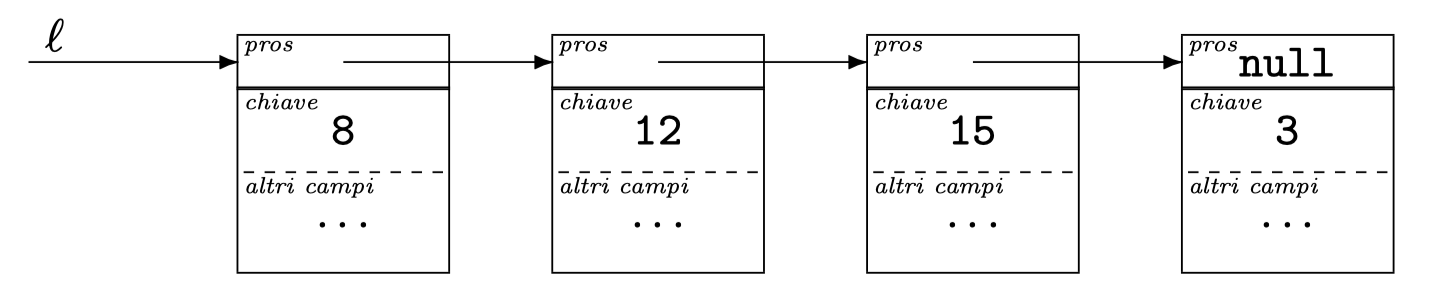
\includegraphics[width=\textwidth]{lista.png}
\end{figure}

\subsection{Operazioni}
Vediamo ora l'implementazione di alcune operazioni che si possono effettuare
sulle liste concatenate lineari ordinate e non.

\begin{figure}[h]
    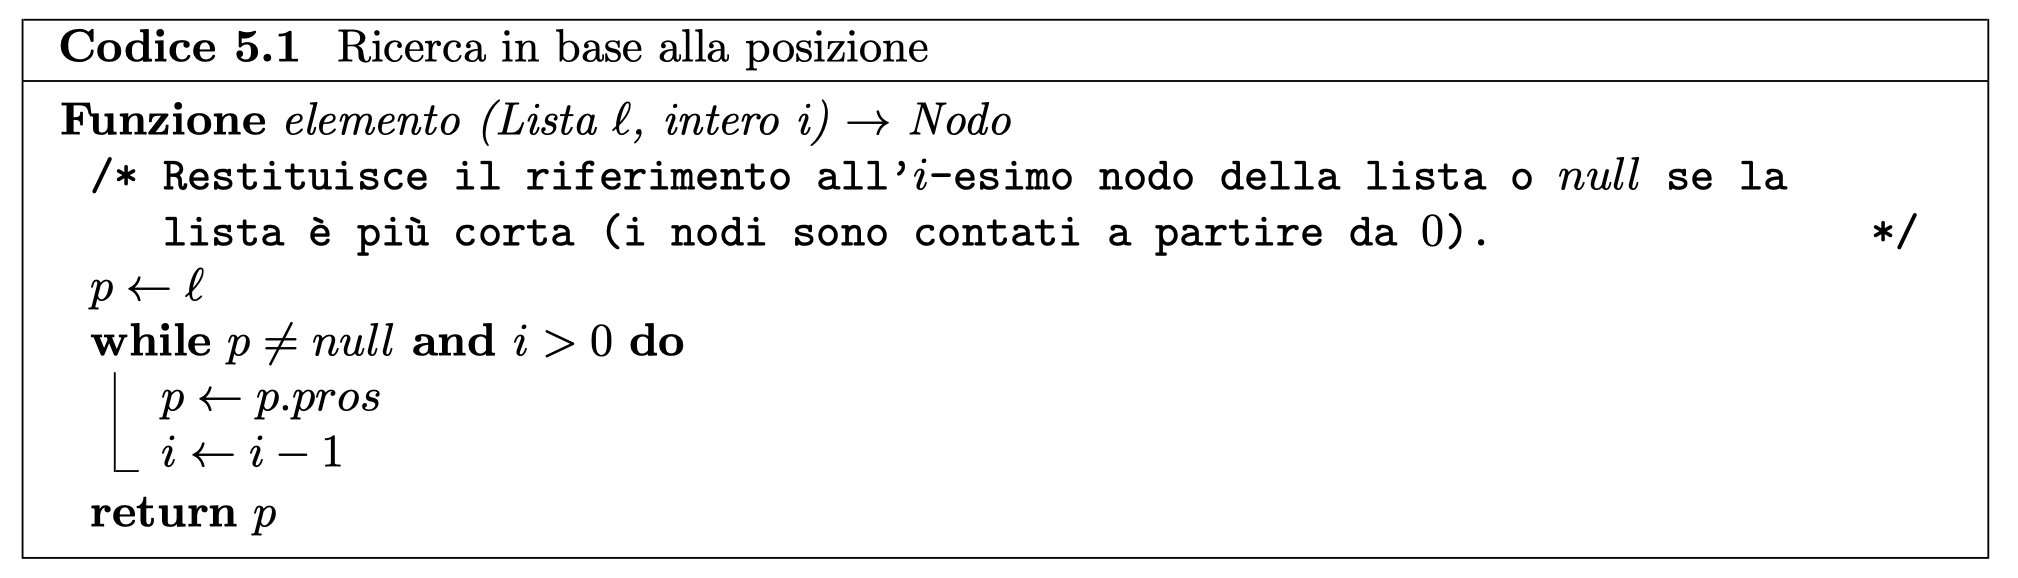
\includegraphics[width=\textwidth]{ricerca_posizione_lista.png}
\end{figure}

\begin{figure}[h]
    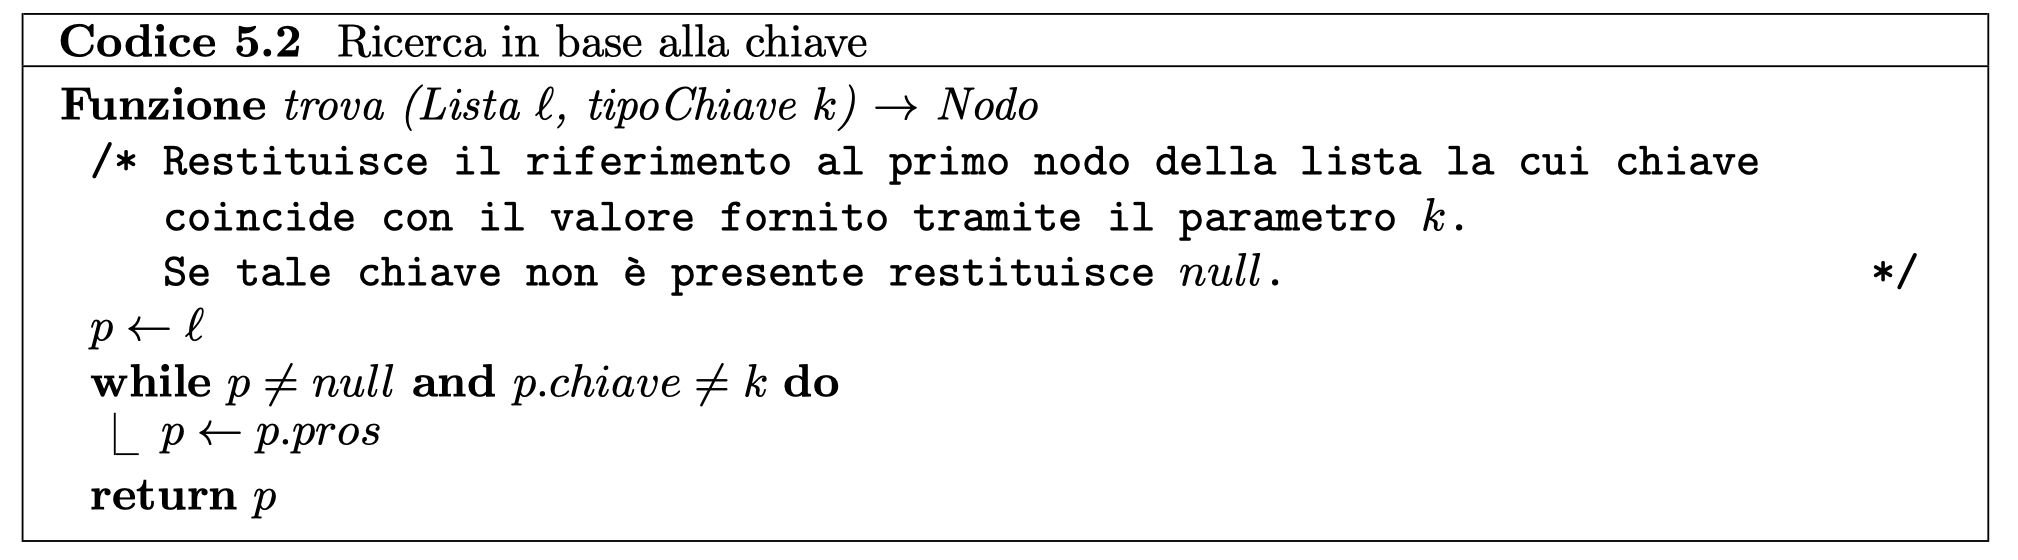
\includegraphics[width=\textwidth]{ricerca_chiave_lista.png}
\end{figure}

\begin{figure}[h]
    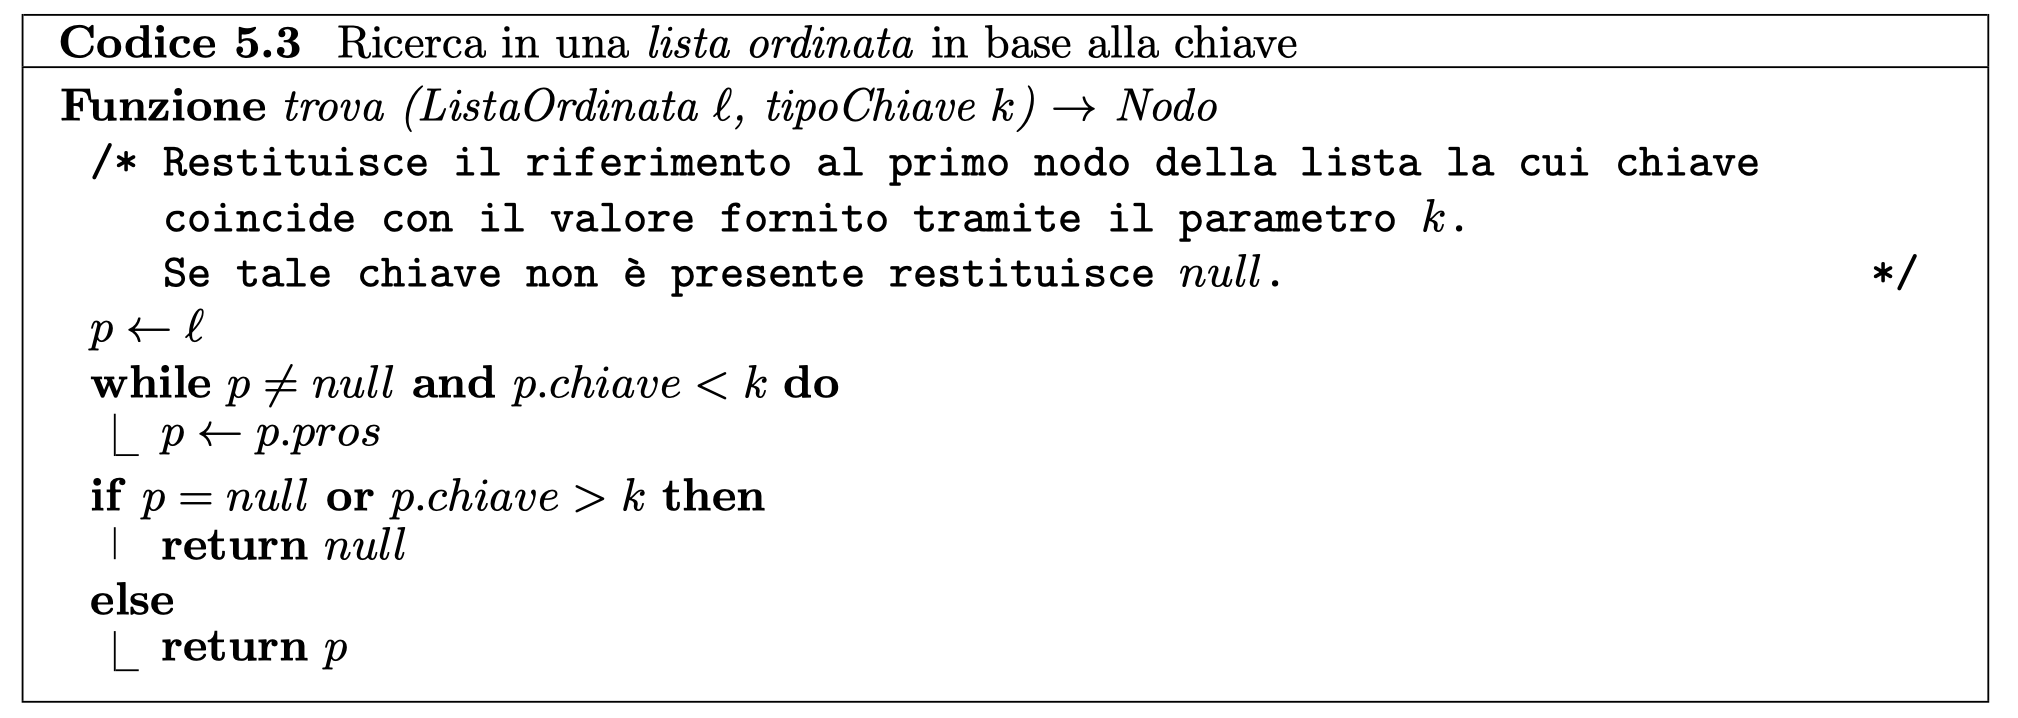
\includegraphics[width=\textwidth]{ricerca_chiave_lista_ordinata.png}
\end{figure}

\begin{figure}[h]
    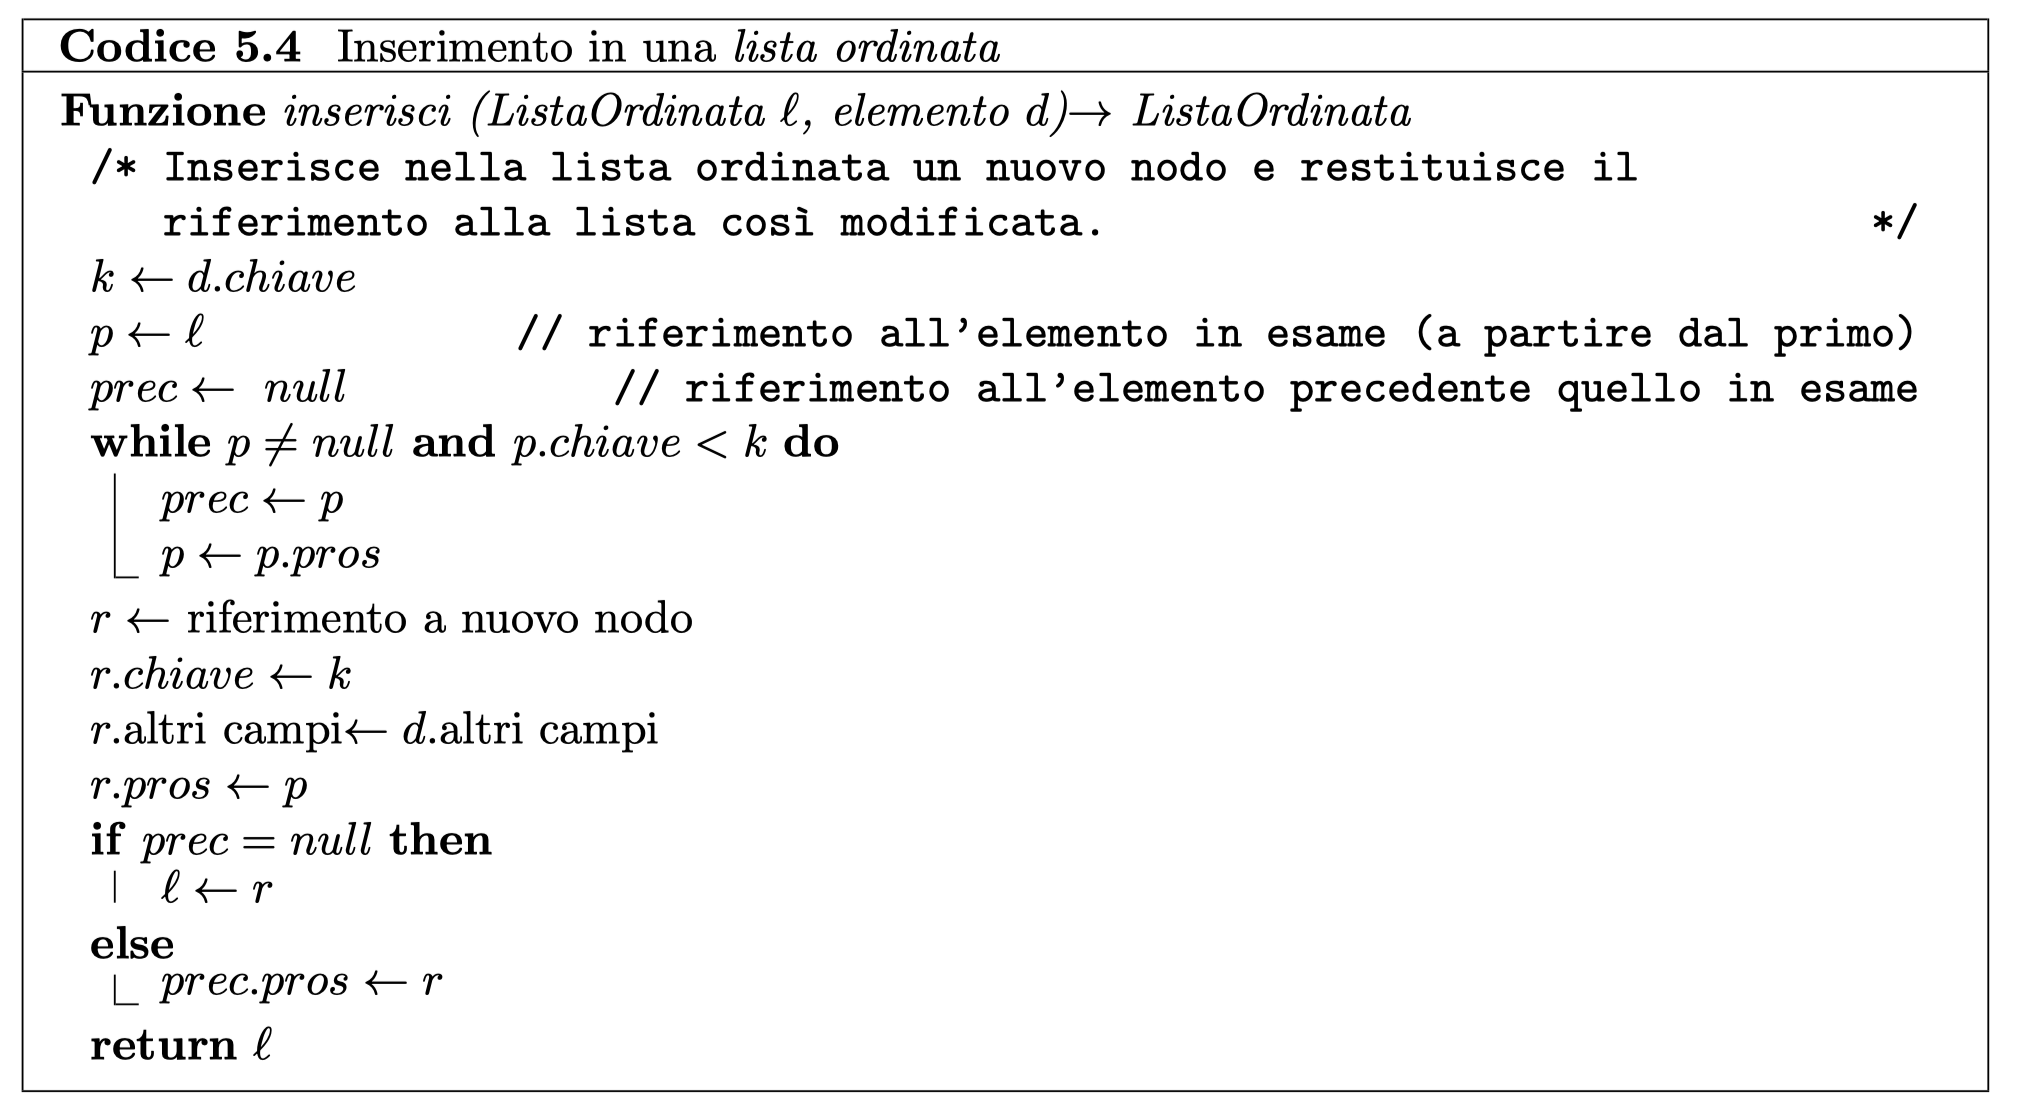
\includegraphics[width=\textwidth]{inserimento_lista_ordinata.png}
\end{figure}

\begin{figure}[h]
    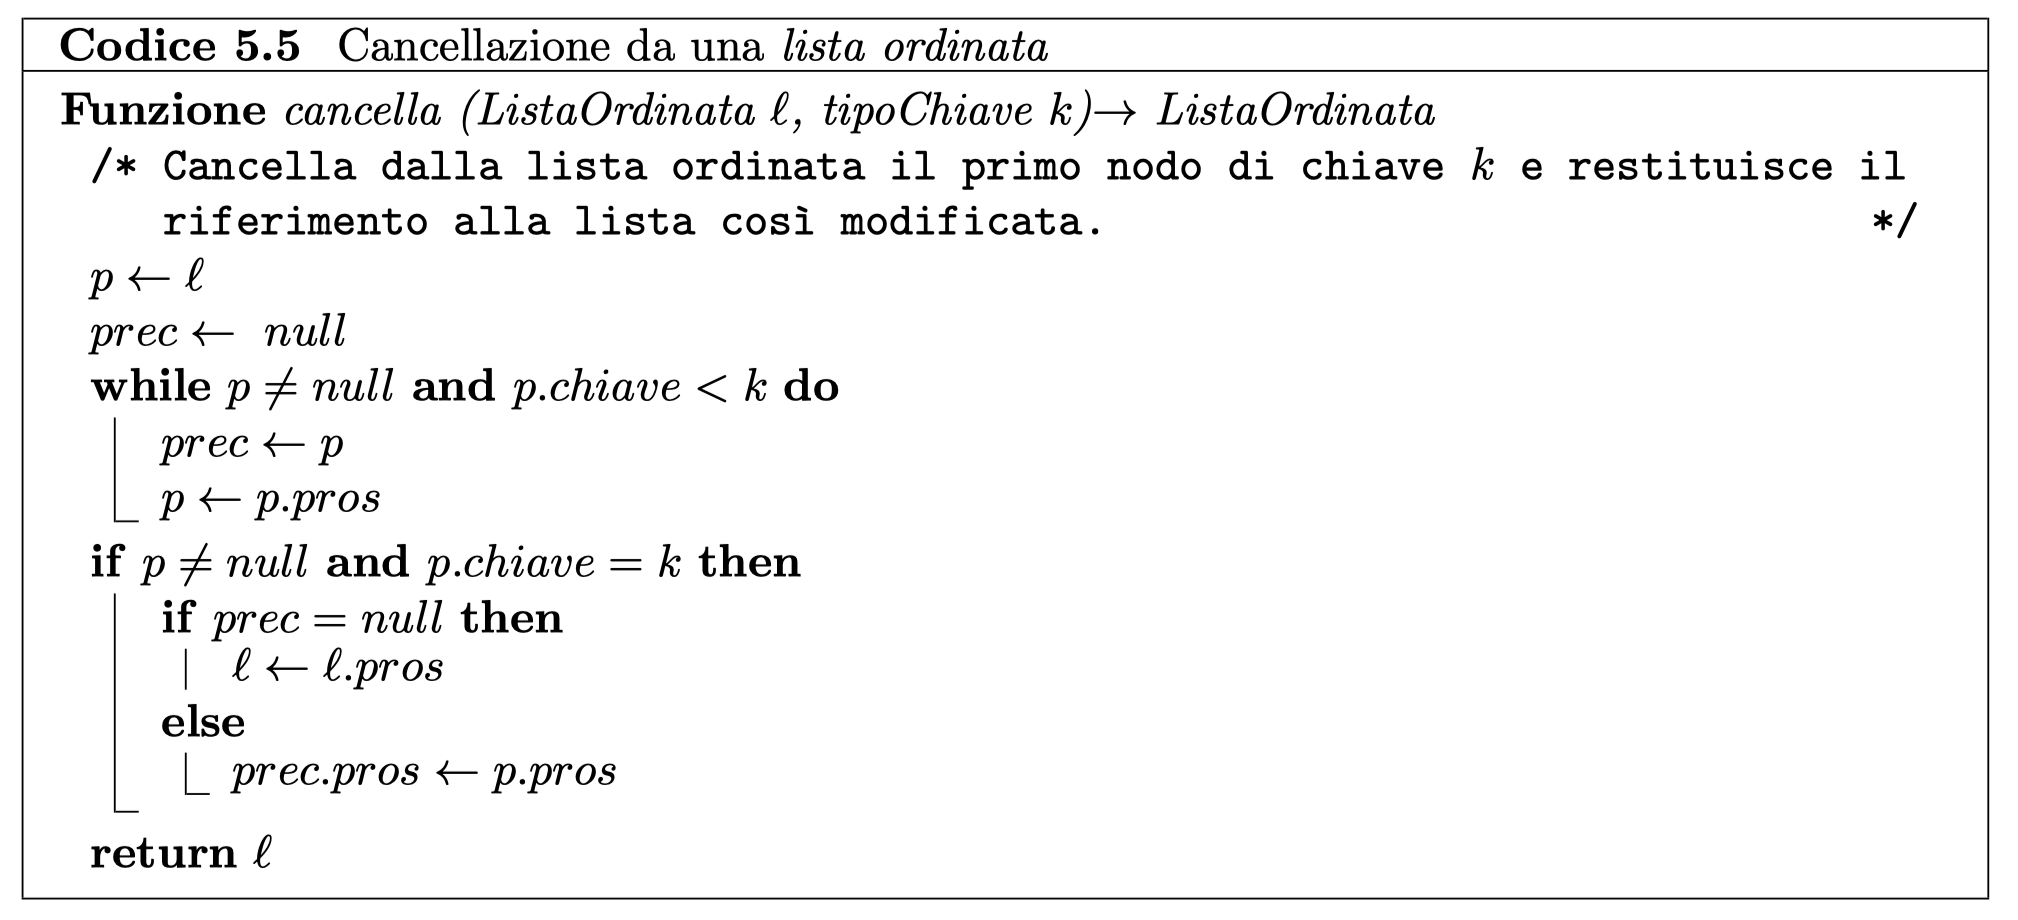
\includegraphics[width=\textwidth]{cancellazione_lista_ordinata.png}
\end{figure}
\clearpage
\section{Stack (Pila)}
Le pile sono delle strutture dati con organizzazione {\textbf{LIFO}}
(Last-In-First-Out).\newline
Possono essere implementate tramite array o tramite liste lineari. Sono
preferibili le liste concatenate singolarmente. \\[2pt]

\begin{wrapfigure}{r}{7cm}
    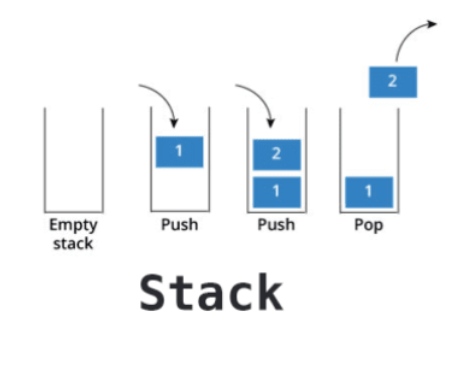
\includegraphics{stack.png}
\end{wrapfigure}


Le operazioni che possono essere eseguite su una pila sono:
\begin{itemize}
    \item {\texttt{isEmpty() $\rightarrow$ boolean}} restituisce \verb|true| se la pila è vuota, \verb|false| altrimenti
    \item {\texttt{push(elemento)}} aggiunge un elemento alla pila
    \item {\texttt{pop() $\rightarrow$ elemento}} rimuove il primo elemento dalla pila e lo restituisce
    \item {\texttt{top() $\rightarrow$ elemento}} restituisce il primo elemento della pila
\end{itemize}


\begin{algorithm}
    \caption{isEmpty}
    \Indm{\textbf{Funzione}} {\emph{isEmpty}}() $\rightarrow$ {\emph{boolean}}\\
       \Indp\eIf{$top = null$}{\Return{$true$}}{\Return{$false$}}
\end{algorithm}

\begin{algorithm}
    \caption{push}
    \Indm\textbf{Procedura} \emph{push}(elemento \emph{x})\\
    \Indp$r$ $\leftarrow$ riferimento ad un nuovo nodo\\
    $r.dato$ $\leftarrow$ $x$\\
    $r.pros$ $\leftarrow$ $top$\\
    $top$ $\leftarrow$ $r$\\
    
\end{algorithm}

\begin{algorithm}
    \caption{top}
    \Indm\textbf{Funzione} \emph{top}() $\rightarrow$ elemento\\
    \Indp\Return{$top.dato$}
\end{algorithm}
\text{}\\[30pt]

\begin{algorithm}
    \caption{pop}
    \Indm\textbf{Funzione} \emph{pop}() $\rightarrow$ elemento\\
    \Indp$x$ $\leftarrow$ $top.dato$\\
    $top$ $\leftarrow$ $top.pros$\\
    \Return{$x$}
\end{algorithm}
\section{Queue (Coda)}
Le code sono delle strutture dati con organizzazione {\textbf{FIFO}}
(First-In-First-Out).
Possono essere implementate tramite array o tramite liste concatenate. Sono 
preferibili le liste doppiamente concatenate.\newline
\begin{wrapfigure}{r}{7cm}
    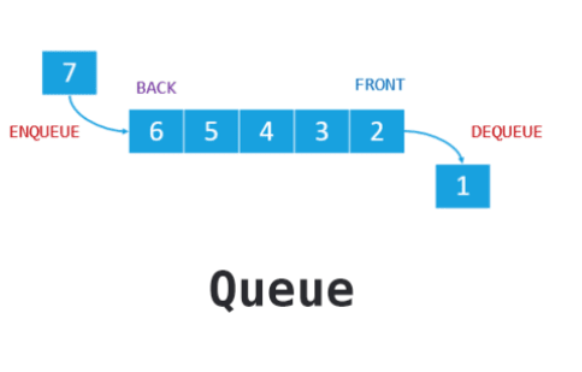
\includegraphics{queue.png}
\end{wrapfigure}

Le operazioni che possono essere eseguite su una coda sono:
\begin{itemize}
    \item {\texttt{isEmpty() $\rightarrow$ boolean}} restituisce \verb|true| se la coda è vuota, \verb|false| altrimenti
    \item {\texttt{enqueue(elemento)}} aggiunge un elemento alla coda
    \item {\texttt{dequeue() $\rightarrow$ elemento}} rimuove il primo elemento dalla coda e lo restituisce
    \item {\texttt{first() $\rightarrow$ elemento}} restituisce il primo elemento della coda
\end{itemize}

\begin{algorithm}
    \caption{isEmpty}
    \Indm{\textbf{Funzione}} {\emph{isEmpty}}() $\rightarrow$ {\emph{boolean}}\\
       \Indp\eIf{$primo = null$}{\Return{$true$}}{\Return{$false$}}
\end{algorithm}

\begin{algorithm}
    \caption{first}
    \Indm\textbf{Funzione} \emph{first}() $\rightarrow$ elemento\\
    \Indp\Return{$primo.dato$}
\end{algorithm}

\begin{algorithm}
    \caption{dequeue}
    \Indm\textbf{Funzione} \emph{dequeue}() $\rightarrow$ elemento\\
    \Indp$x$ $\leftarrow$ $primo.dato$\\
    $primo$ $\leftarrow$ $primo.pros$\\
    \If{$primo = null$}{$ultimo \leftarrow null$}
    \Return{$x$}
\end{algorithm}

\begin{algorithm}
    \caption{enqueue}
    \Indm\textbf{Procedura} \emph{enqueue}(elemento \emph{x})\\
    \Indp$r$ $\leftarrow$ riferimento ad un nuovo nodo\\
    $r.dato$ $\leftarrow$ $x$\\
    $r.pros$ $\leftarrow$ $null$\\
    \eIf{$primo = null$}{
        $primo \leftarrow r$\\
        $ultimo \leftarrow r$
    }{
        $ultimo.pros \leftarrow r$\\
        $ultimo \leftarrow r$
    }
    
\end{algorithm}


\clearpage
\section{Alberi}
La definizione formale di albero sarà data quando tratteremo i grafi. Per ora 
diciamo che gli alberi sono strutture formate da nodi, simili alle liste, ma
con una rappresentazione gerarchica dei dati.
\begin{wrapfigure}{r}{7cm}
    \caption{Esempio di albero binario}
    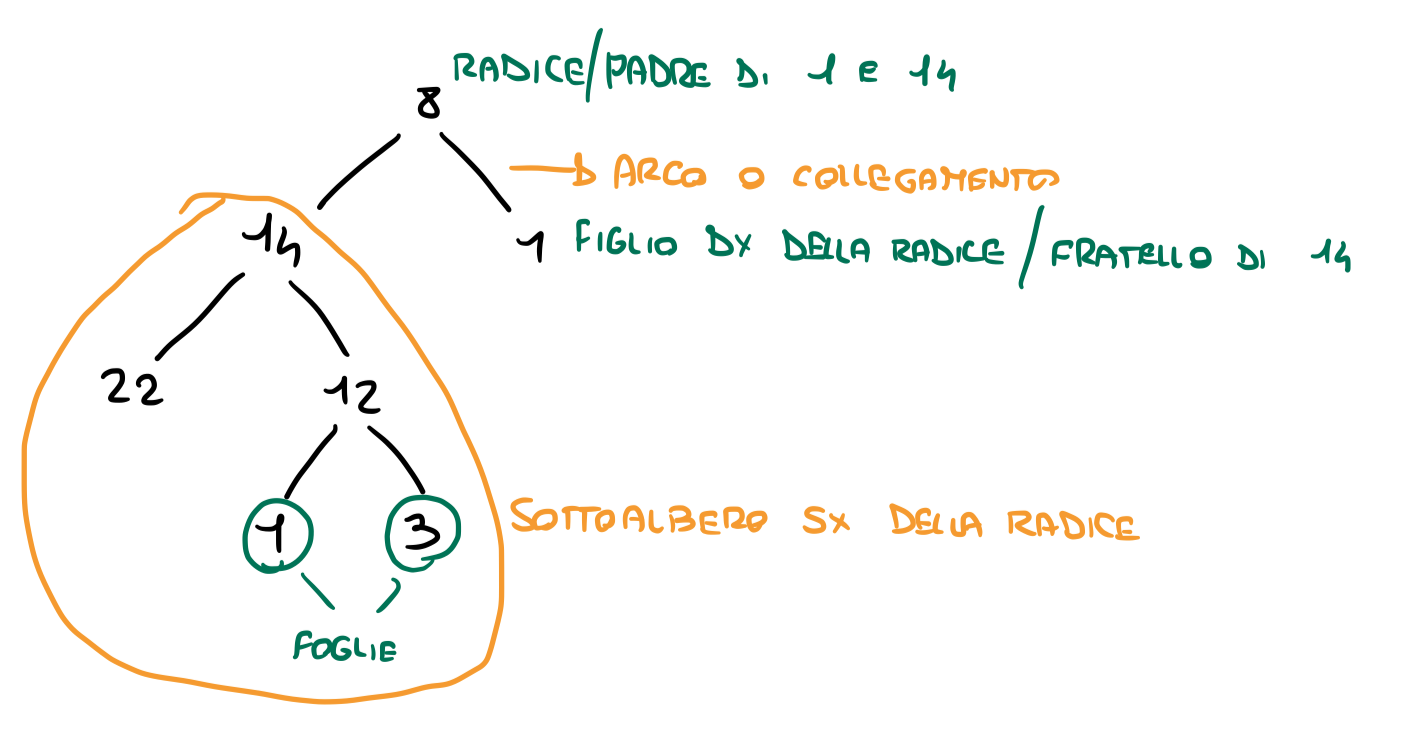
\includegraphics[scale = 0.3]{albero.png}
\end{wrapfigure}
La \emph{radice} è il nodo che sta in cima alla gerarchia. Ogni nodo ha un solo nodo 
{\emph{padre}} ma può avere un qualsiasi numero di \emph{figli}. La radice non ha un nodo padre.
I nodi che si trovano al livello più basso della gerarchia (i nodi che non hanno figli) sono detti
\emph{foglie}.
I collegamenti tra nodi sono detti \emph{archi}.\\
Un albero in cui ogni nodo può avere al massimo due figli è detto \emph{albero binario}
Possiamo dare una definizione ricorsiva di albero:\\
Un \textbf{albero binario} è:
\begin{itemize}
    \item una struttura vuota\\
    oppure 
    \item un nodo (radice) con associati due alberi binari detti \emph{sottoalbero sinistro} e \emph{sottoalbero destro}.
\end{itemize}
La radice di un albero ha \emph{profondità} pari a 0, i nodi di profondità $k$ 
hanno profondità $k + 1$.\\
Si definisce {\emph{altezza}} di un albero la massima profondità dei nodi.\\
Il \emph{grado} di un nodo è il massimo di figli che può avere quel nodo.\\
Alcuni esempi di dati rappresentati tramite alberi possono essere l'indice di un 
libro, uno schema del regno animale ma anche operazioni aritmetiche e in informatica
le chiamate ricorsive.
\subsection{Rappresentazione di alberi}
\subsubsection{Vettore dei padri}
\begin{figure}[h]
    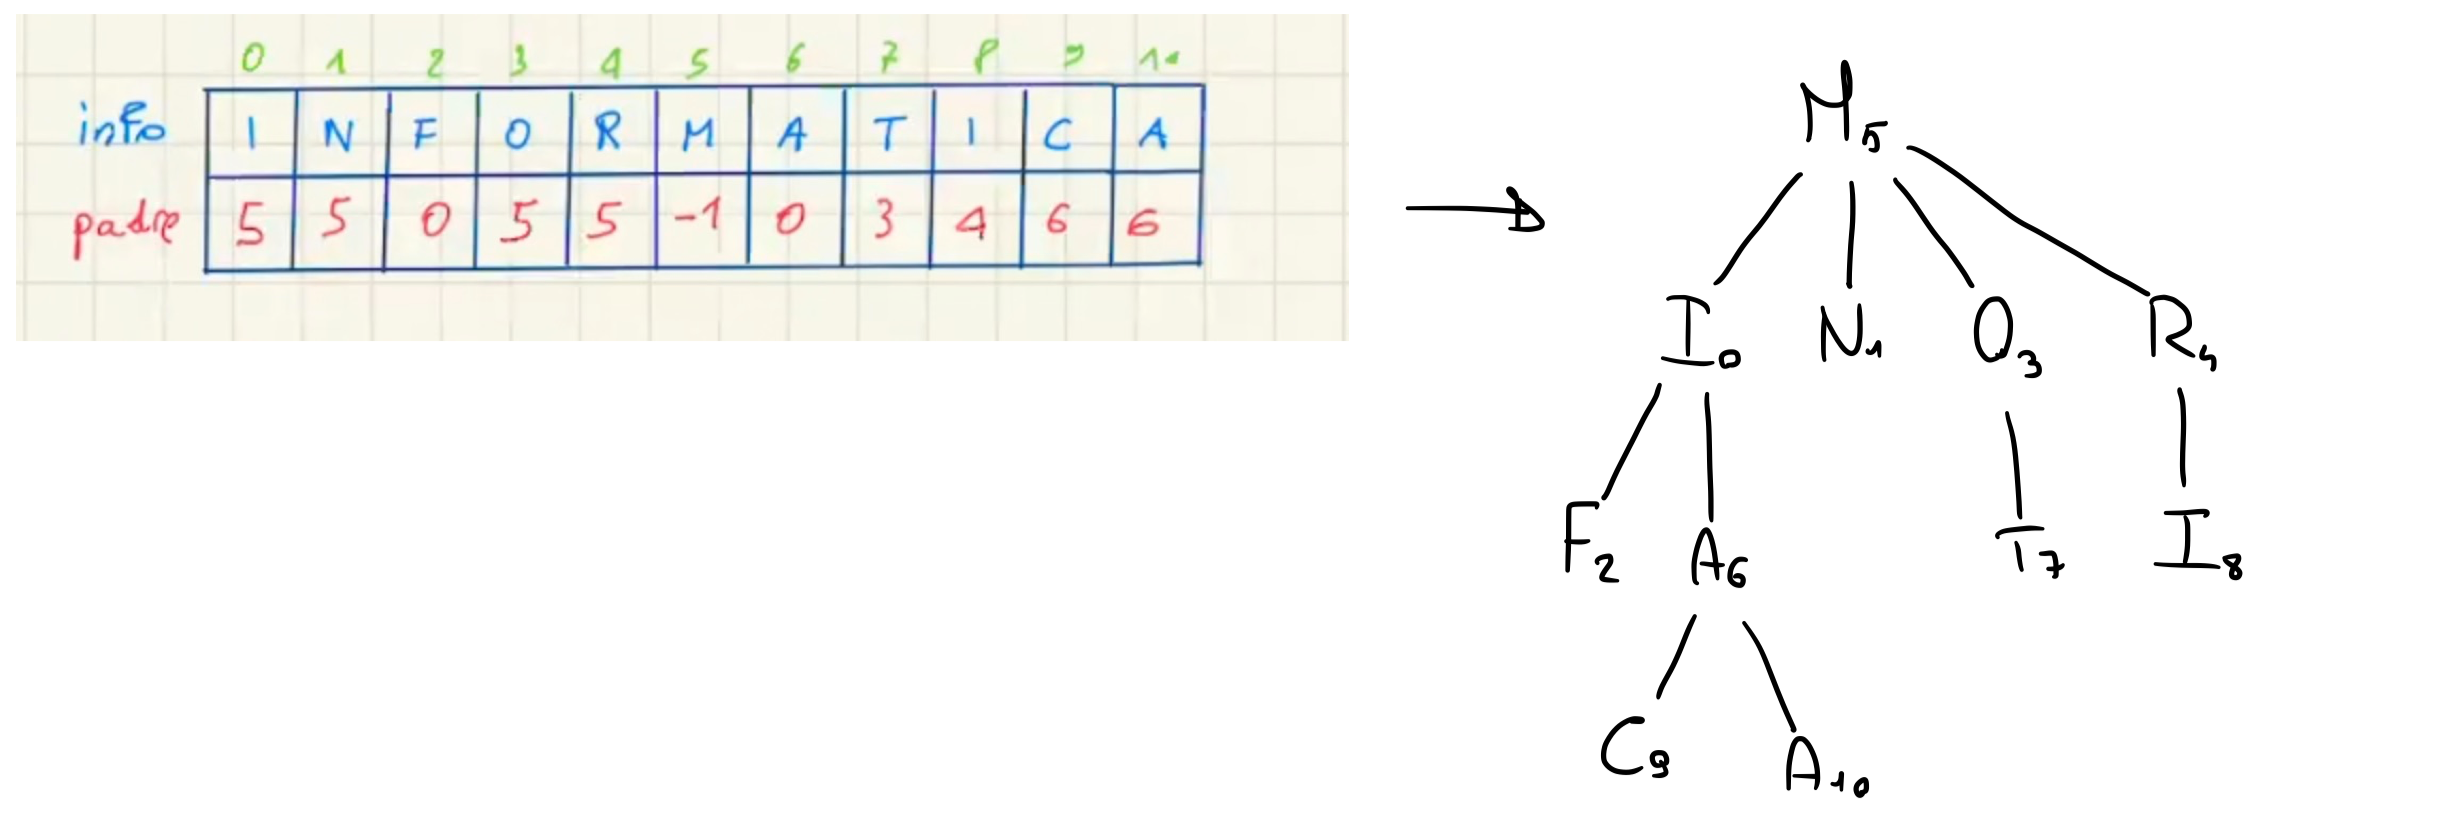
\includegraphics[width=\textwidth]{vettore_padri.png}
\end{figure}
\clearpage

\subsubsection{Rappresentazioni collegate: puntatori ai figli e lista dei fratelli}
\begin{figure}[h]
    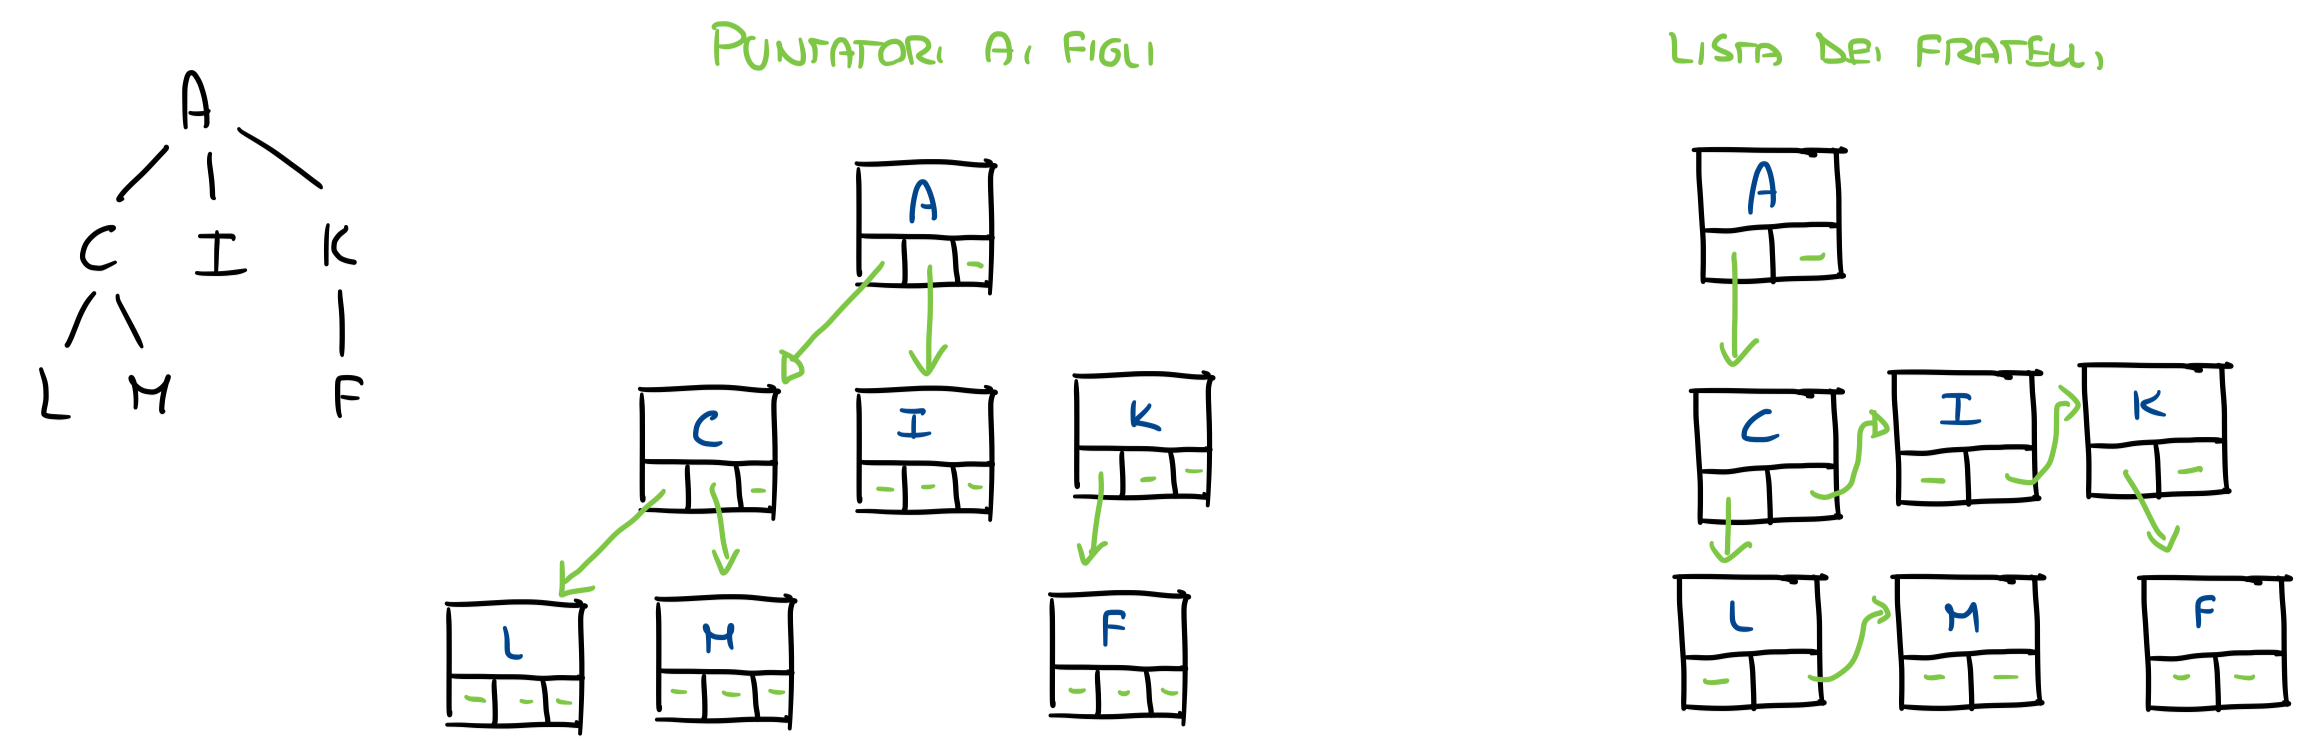
\includegraphics[width=\textwidth]{lista_fratelli.png}
\end{figure}

\subsection{Visite di alberi}
Vediamo ora alcune strategie per attraversare tutti i nodi di un albero.
\begin{algorithm}
    \caption{Visita generica}
    \Indm\textbf{Algoritmo} \emph{visitaGenerica}(\emph{AlberoBinario r})\\
    \Indp$S$ $\leftarrow$ $\lbrace r \rbrace$\\
    \While{$S \neq \emptyset$}{
        preleva un nodo $v$ da $S$\\
        visita $v$\\
        $S$ $\leftarrow$ $S$ $\cup$ $\lbrace$ figli di $v$ $\rbrace$
    }
\end{algorithm}

\begin{algorithm}
    \caption{Visita in ampiezza}
    \Indm\textbf{Algoritmo} \emph{visitaAmpiezza}(\emph{AlberoBinario r})\\
    \Indp$C$ $\leftarrow$ coda vuota\\
    $C.enqueue(r)$\\
    \While{\textbf{not} $C$.isEmpty()}{
        $n$ $\leftarrow$ $C.dequeue$\\
        \If{$n \neq null$}{
            visita il nodo associato a $n$\\
            $C.enqueue$($n.sx$)\\
            $C.enqueue$($n.dx$)\\
        }
    }
\end{algorithm}

\begin{algorithm}
    \caption{Visita in profondità}
    \Indm\textbf{Algoritmo} \emph{visitaProfondità}(\emph{AlberoBinario r})\\
    \Indp$P$ $\leftarrow$ pila vuota\\
    $P.push(r)$\\
    \While{\textbf{not} $P$.isEmpty()}{
        $n$ $\leftarrow$ $P.pop$\\
        \If{$n \neq null$}{
            visita il nodo associato a $n$\\
            $P.push$($n.sx$)\\
            $P.push$($n.dx$)\\
        }
    }
\end{algorithm}

\begin{algorithm}
    \caption{Visita in ordine anticipato}
    \Indm\textbf{Algoritmo} \emph{visitaPreOrder}(\emph{AlberoBinario r})\\
    \Indp\If{$r \neq null$}{
        visita la radice\\
        \emph{visitaPreOrder(r.sx)}\\
        \emph{visitaPreOrder(r.dx)}\\
    }
\end{algorithm}

\begin{algorithm}
    \caption{Visita in ordine simmetrico}
    \Indm\textbf{Algoritmo} \emph{visitaInOrder}(\emph{AlberoBinario r})\\
    \Indp\If{$r \neq null$}{
        \emph{visitaPreOrder(r.sx)}\\
        visita la radice\\
        \emph{visitaPreOrder(r.dx)}
    }
\end{algorithm}

\begin{algorithm}
    \caption{Visita in ordine posticipato}
    \Indm\textbf{Algoritmo} \emph{visitaPreOrder}(\emph{AlberoBinario r})\\
    \Indp\If{$r \neq null$}{
        \emph{visitaPreOrder(r.sx)}\\
        \emph{visitaPreOrder(r.dx)}\\
        visita la radice
    }
\end{algorithm}

\begin{algorithm}
    \caption{Numero nodi di un albero}
    \Indm\textbf{Funzione} \emph{numeroNodi}(\emph{AlberoBinario r}) $\rightarrow intero$\\
    \Indp\eIf{$r = null$}{
        \Return{0}
    }
    {
        $nsx \leftarrow numeroNodi(r.sx)$\\
        $ndx \leftarrow numeroNodi(r.dx)$\\
        \Return{1 + $nsx$ + $ndx$}
    }
\end{algorithm}
\clearpage



\section{Alberi binari di ricerca}
Gli alberi binari di ricerca sono alberi in cui per ogni nodo $n$: 
\begin{enumerate}
    \item Il valore di ogni chiave contenuta nel sottoalbero sinistro di $n$ è minore o uguale alla chiave di $n$
    \item Il valore di ogni chiave contenuta nel sottoalbero destro di $n$ è maggiore della chiave di $n$
\end{enumerate}
Una visita in ordine simmetrico di un A.B.R. produce un elenco ordinato per chiave.\\
Se devo trovare il nodo con chiave massima scendo tutto a destra, per quello di chiave minima tutto a sinistra.\\
Il costo di inserimento, ricerca e cancellazione è $O(altezza)$.
Il massimo numero di nodi di un albero di altezza $h$ è $2^{h+1}-1$, quindi:
\begin{itemize}
    \item $h + 1 \le n \le 2^{h+1}-1$
    \item $\log_2(n+1) - 1 \le h \le n - 1$
\end{itemize}
Vogliamo fare in modo che l'albero rimanga più bilanciato possibile in modo
da evitare il caso peggiore.

\subsection{Operazioni}
Vediamo ora l'implementazione di alcune operazioni eseguibili sugli alberi binari di ricerca.
\begin{algorithm}
    \caption{Ricerca del massimo}
    \Indm\textbf{Funzione} \emph{massimo (AlberoRicerca r)} $\rightarrow Nodo$\\
    \Indp\eIf{$r = null$}{\Return $null$}{
        $n \leftarrow r$\\
        \While{$n.dx \neq null$}{
            $n \leftarrow n.dx$
        }
        \Return{$n$}
    }
\end{algorithm}

\begin{algorithm}
    \caption{Ricerca del minimo}
    \Indm\textbf{Funzione} \emph{minimo (AlberoRicerca r)} $\rightarrow Nodo$\\
    \Indp\eIf{$r = null$}{\Return $null$}{
        $n \leftarrow r$\\
        \While{$n.sx \neq null$}{
            $n \leftarrow n.sx$
        }
        \Return{$n$}
    }
\end{algorithm}
\clearpage
\begin{figure}[h]
    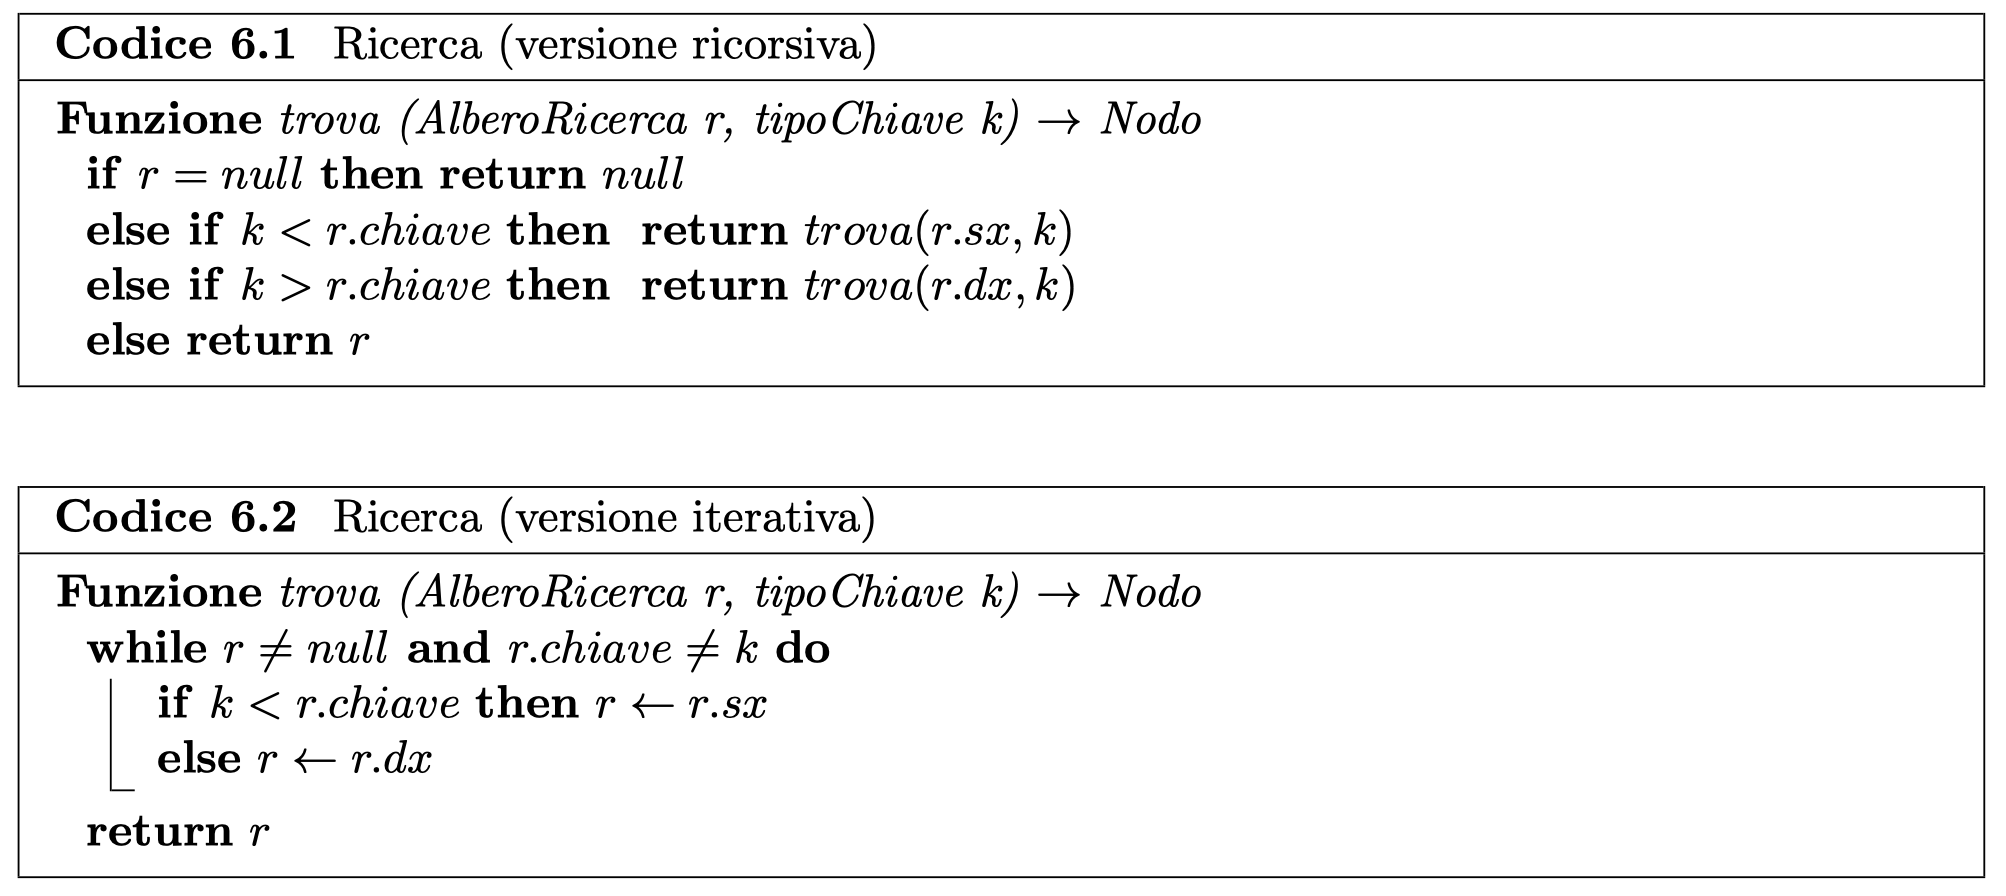
\includegraphics[width=\textwidth]{ricerca_abr.png}
\end{figure}

\begin{figure}[h]
    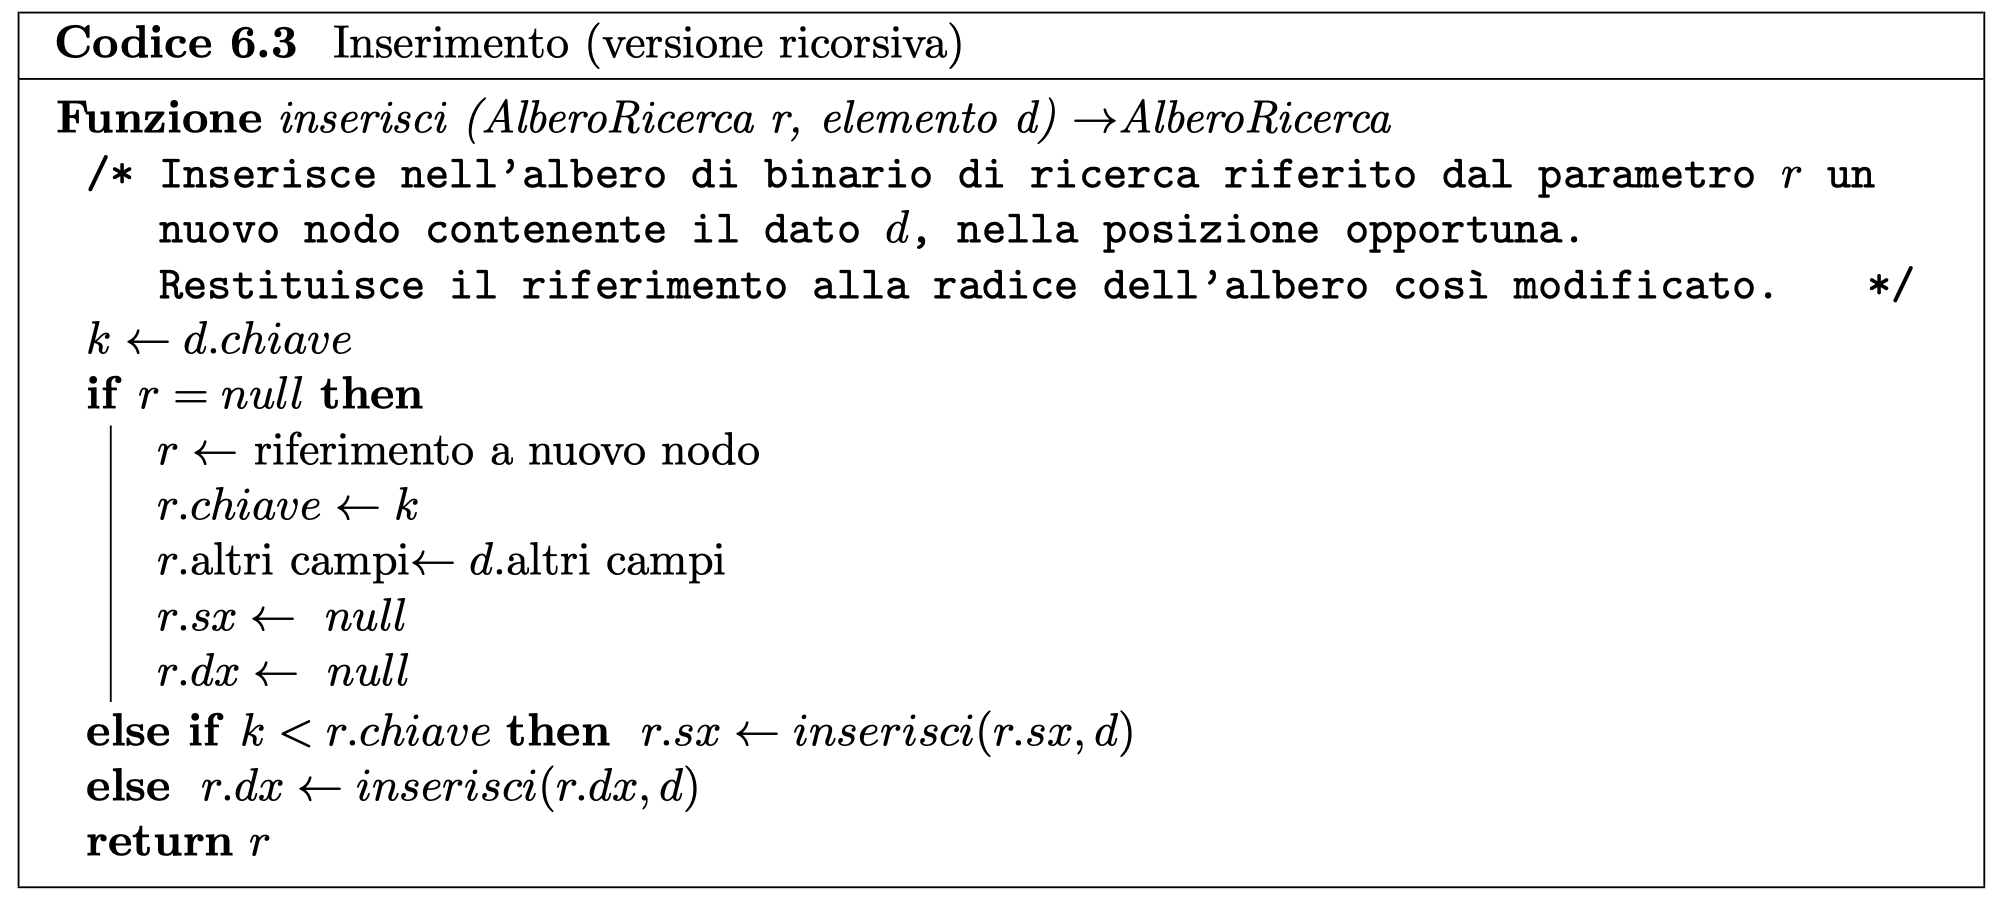
\includegraphics[width=\textwidth]{inserimento_ricorsivo_abr.png}
\end{figure}

\begin{figure}[h]
    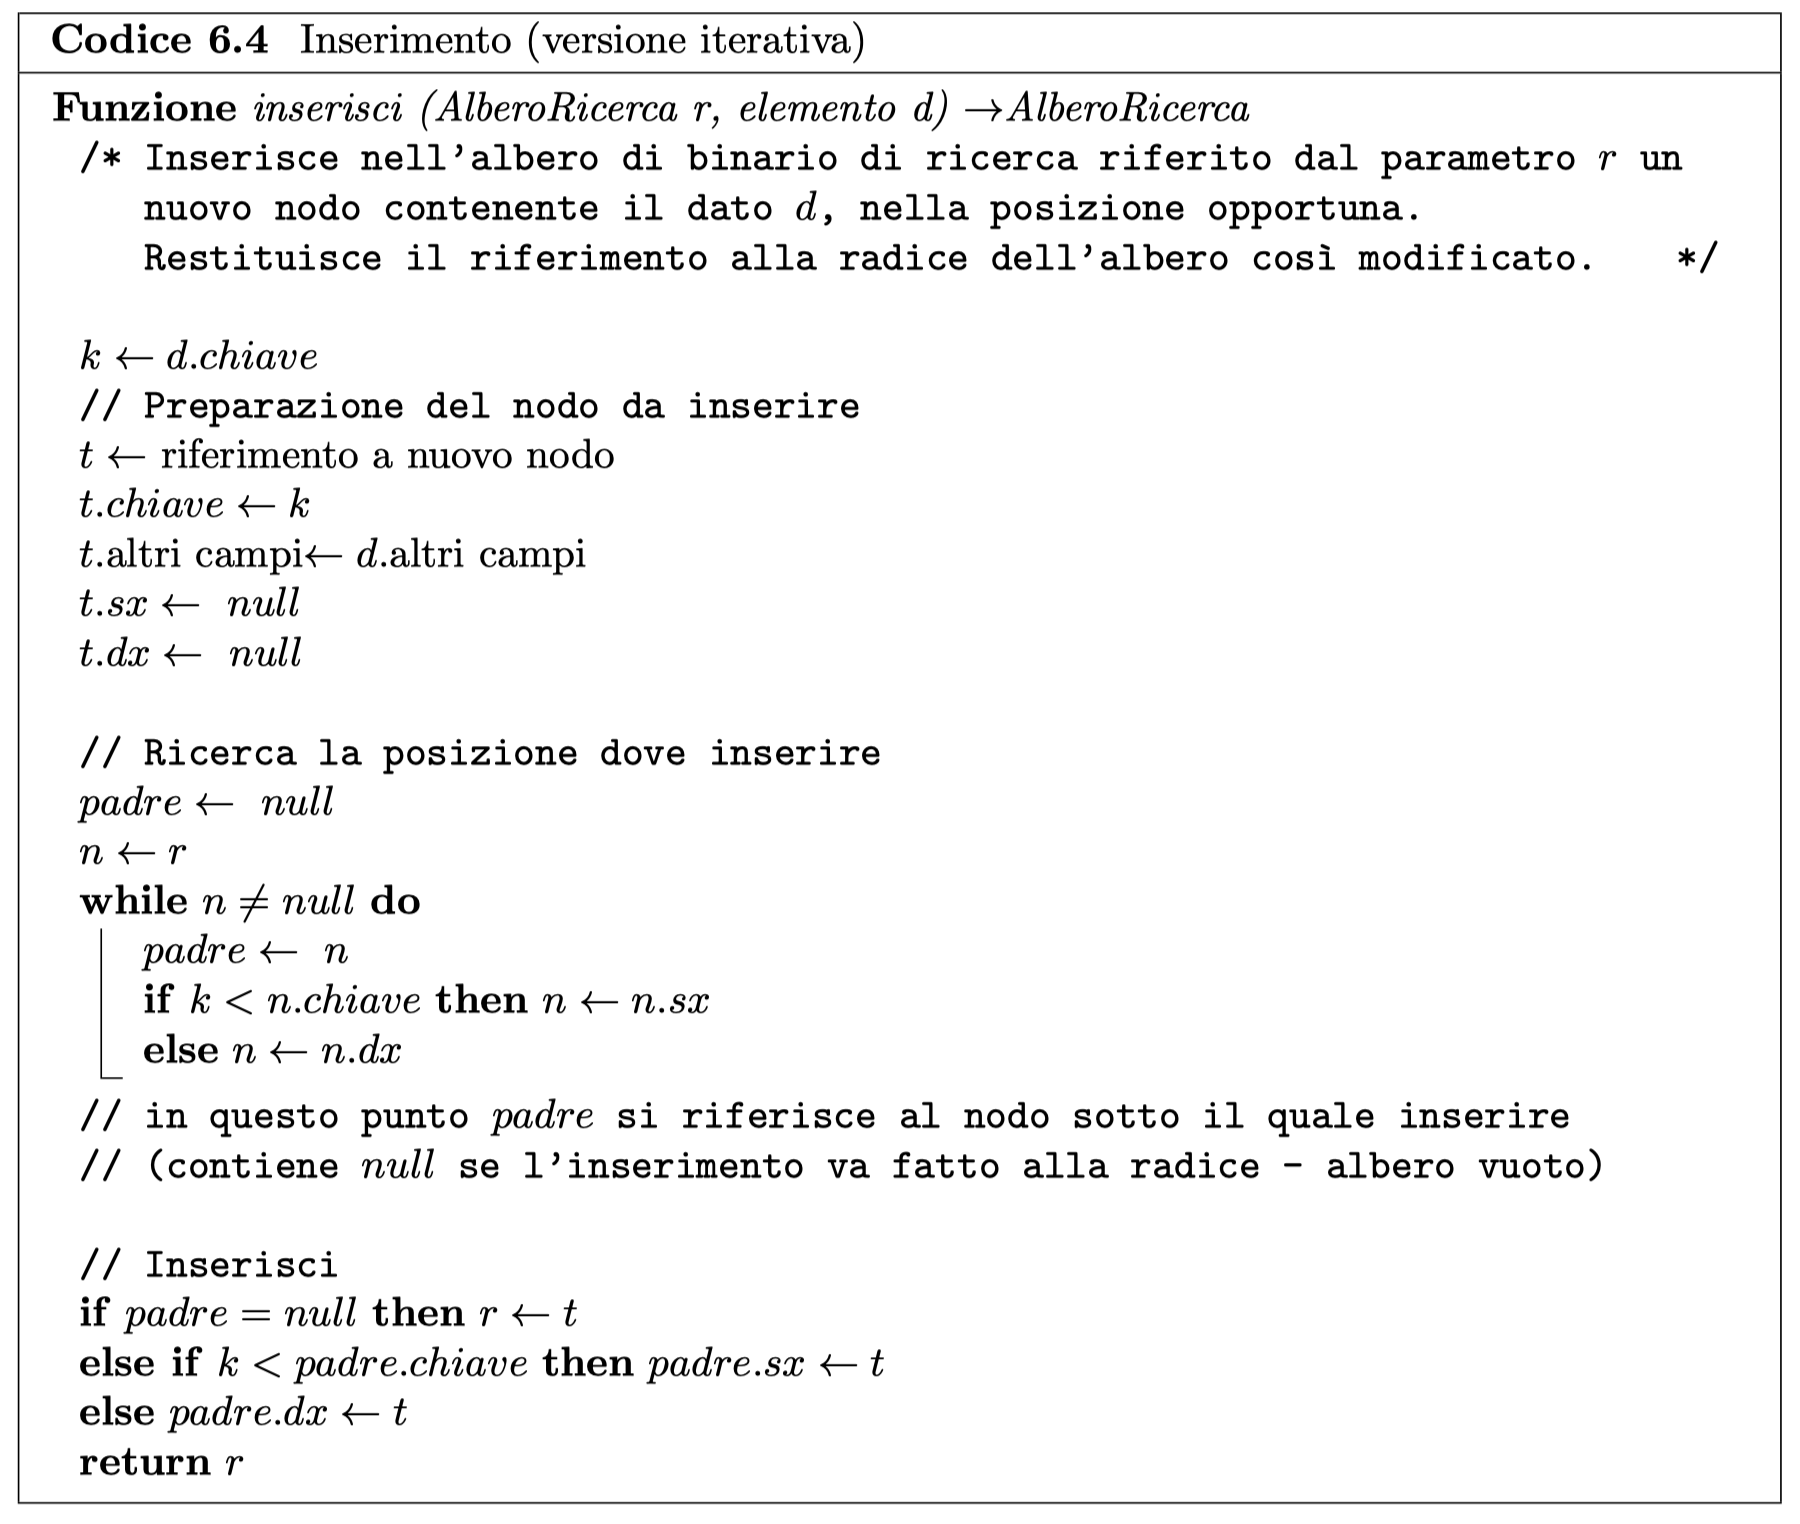
\includegraphics[width=\textwidth]{inserimento_iterativo_abr.png}
\end{figure}

\begin{figure}[h]
    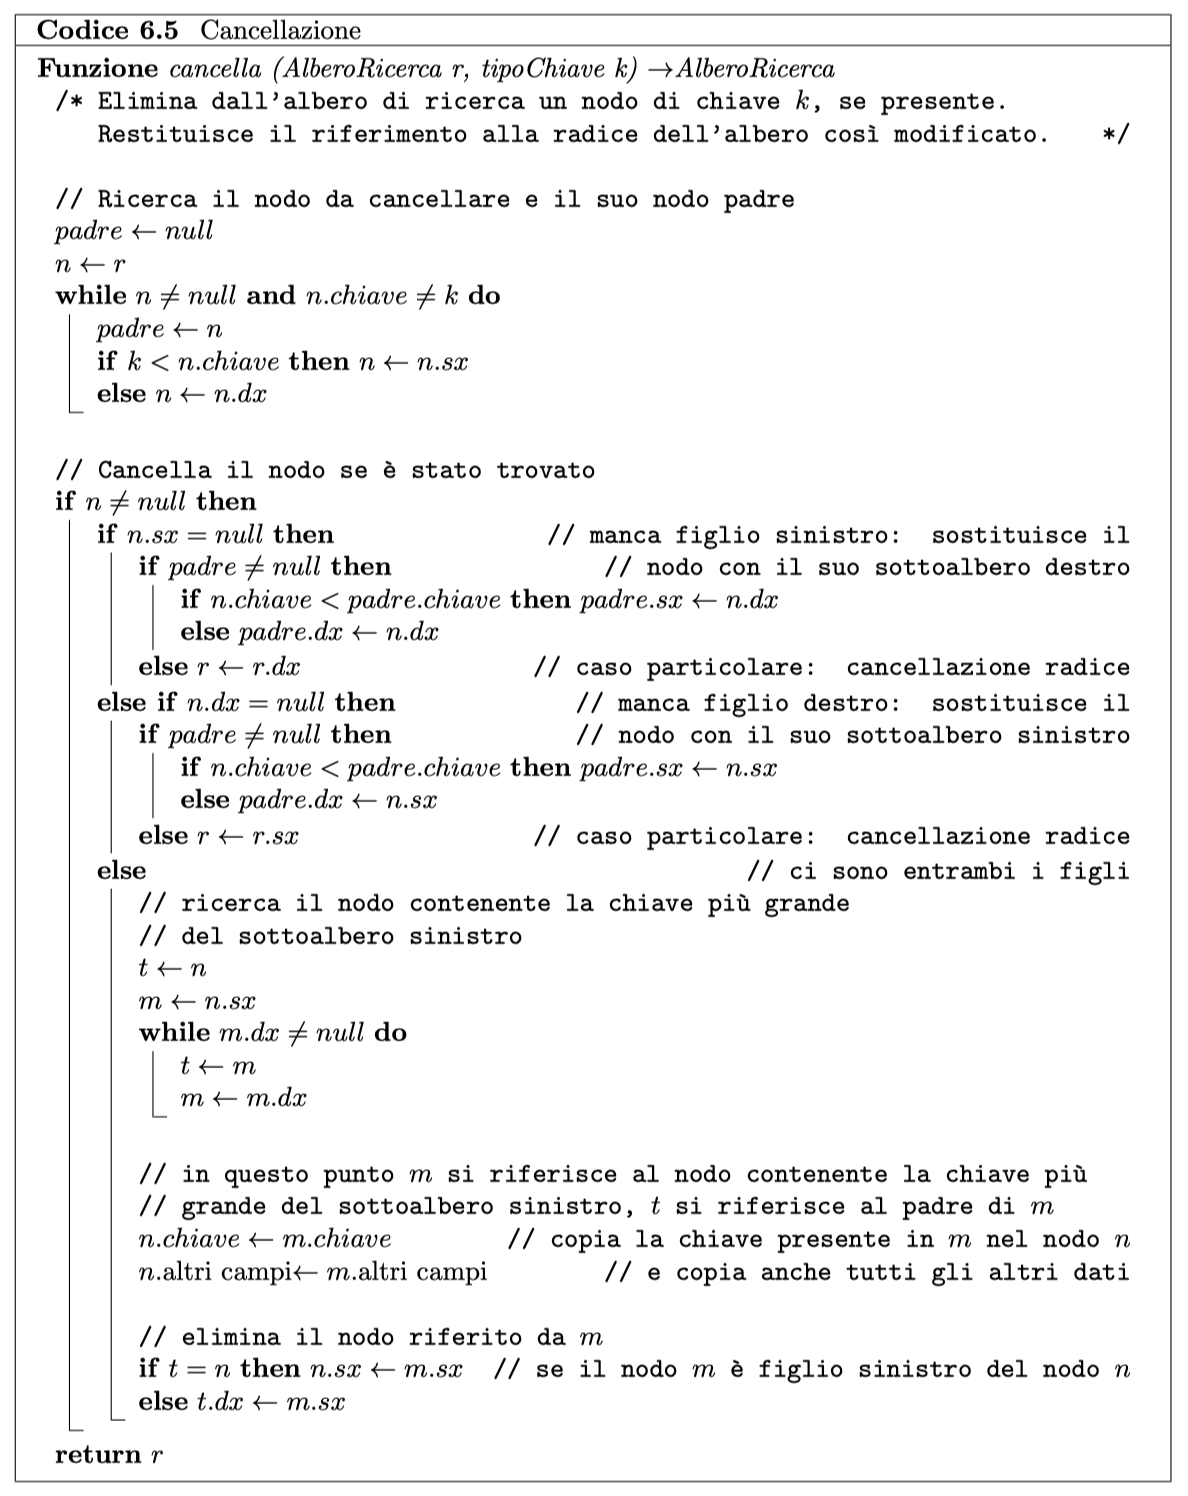
\includegraphics[width=\textwidth]{cancellazione_abr.png}
\end{figure}
\clearpage

\section{Altri tipi di alberi}
\subsection{Alberi perfettamente bilanciati}
Un albero è \emph{perfettamente bilanciato} quando per ogni nodo la differenza tra il 
numero di nodi del sottoalbero sinistro e il numero di nodi del sottoalbero destro
è al massimo 1.
\subsection{Alberi bilanciati in altezza o AVL}
Un albero è \emph{bilanciato in altezza} o \emph{AVL} quando per ogni nodo la differenza
in valore assoluto tra l'altezza del sottoalbero destro e l'altezza del sottoalbero sinistro è
al massimo 1.\\
\textbf{N.B} bilanciato in altezza $\Rightarrow$ bilanciato, ma non viceversa.\\
\textbf{Numero massimo di nodi}: $2^{h+1} - 1$\\[20pt]
\textbf{Numero minimo di nodi}:
\begin{equation*}
    \begin{cases}
        1 & \text{se h = 0}\\
        2 & \text{se h = 1}\\
        1 + n_{h-1}+n_{h-2} & \text{se h $>$ 1}
    \end{cases}
\end{equation*}
\begin{wrapfigure}{r}{7cm}
    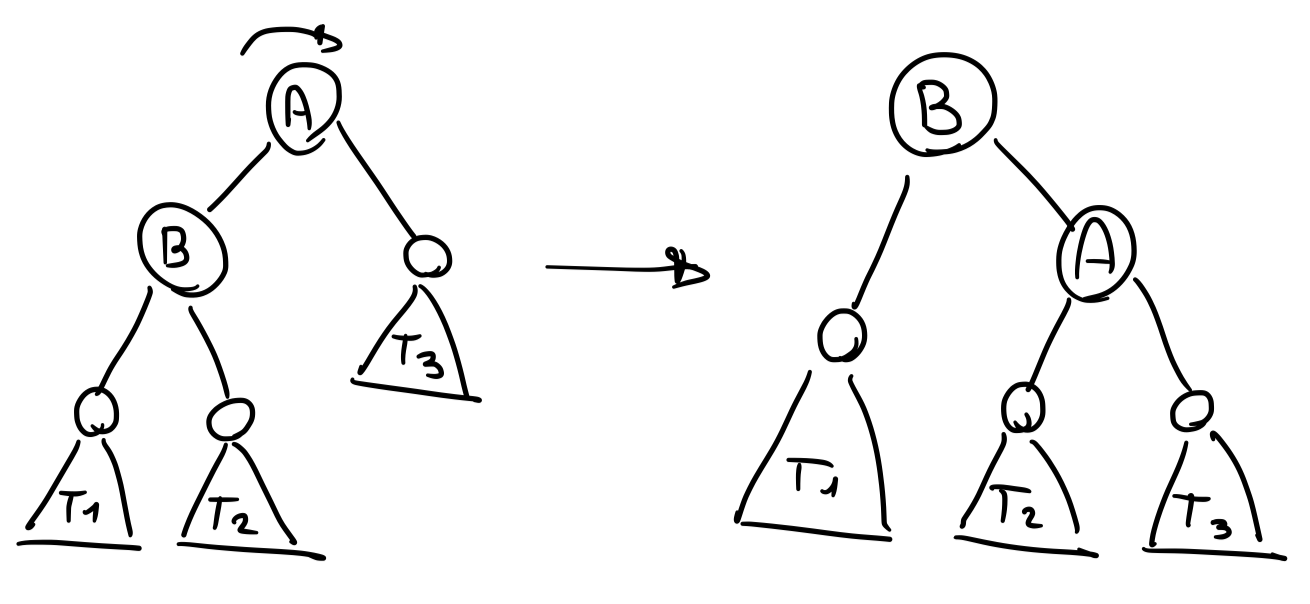
\includegraphics[scale = 0.3]{albero_sbilanciato.png}
\end{wrapfigure}
Un albero AVL con il minimo numero di nodi è detto \emph{albero di Fibonacci}
Nel caso l'albero risulti sbilanciato devo eseguire delle operazioni per sistemarlo.

\subsubsection*{Costo operazioni}
Dato un albero di ricerca di $n$ nodi
\begin{itemize}
    \item Ricerca $O(\log_2 n)$
    \item Inserimento $O(\log_2 n)$
    \item Cancellazione $O(\log_2 n)$
\end{itemize}

\noindent Questa per ora è la struttura con prestazioni migliori per i dizionari, almeno 
finchè non vedremo le tabelle hash più avanti.

\subsection{Alberi 2-3}
Gli \emph{alberi 2-3} sono alberi in cui ogni nodo interno ha 2 o 3 figli
e le foglie sono tutte allo stesso livello. I dati sono memorizzati solo nelle foglie
e i nodi interni contengono solo informazioni di instradamento.
\begin{itemize}
    \item Se la chiave di un nodo interno contiene solo un valore, significa che il nodo ha 2 figli,
        e quel valore è il maggiore del sottoalbero sinistro
    \item Se la la chiave di un nodo interno contiene 2 valori significa che il nodo ha 3 figli, e i due
    valori corrispondono rispettivamente al massimo valore contenuto nel sottoalbero sinistro e al massimo
    valore contenuto nel sottoalbero centrale
\end{itemize} 
    
\begin{figure}[h]
    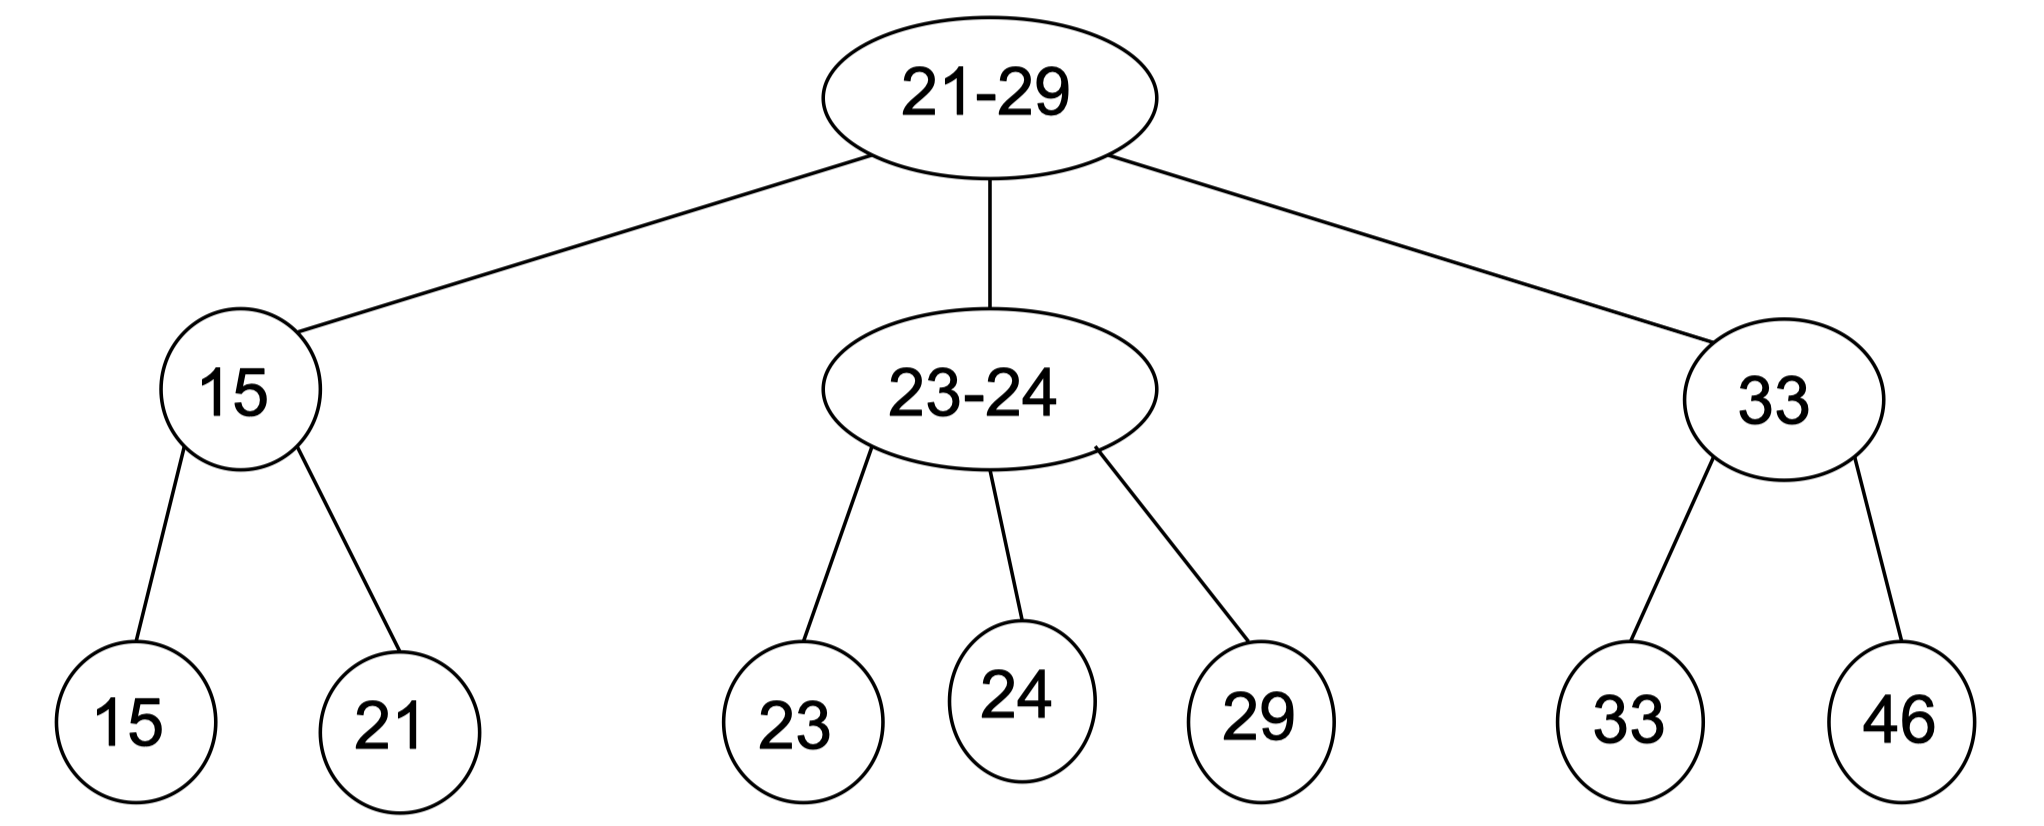
\includegraphics[width = \textwidth]{albero_2-3.png}
\end{figure}

\begin{tabular}{|l|c|c|}
    \hline
    \space & \textbf{min} & \textbf{max}\\
    \hline
    \textbf{Numero nodi} & $2^{h+1}-1$ & $\frac{3^{h+1}-1}{2}$\\
    \hline
    \textbf{Numero foglie} & $2^{h}$ & $3^{h}$\\
    \hline
\end{tabular}
\subsubsection{Operazioni}

\begin{algorithm}
    \caption{Ricerca di un dato}
    \Indm\textbf{Funzione} \emph{trova(albero2-3 r, tipoChiave k)} $\rightarrow$ \emph{foglia}\\
    \Indp$n \leftarrow r$\\
    \While{n si riferisce ad un nodo interno}{
        \eIf{$k \le n.s$}{$n \leftarrow n.sx$}{$n \leftarrow n.dx$}
    }
    \eIf{$n.chiave = k$}{ \Return $n$}{\Return{null}}
\end{algorithm}

\noindent Per inserimenti e cancellazioni è utile tenere in ogni nodo un puntatore al nodo padre.
Quando un nodo ha già 3 figli e devo inserirne un altro, faccio uno \emph{split}.
\clearpage
\begin{figure}[h]
    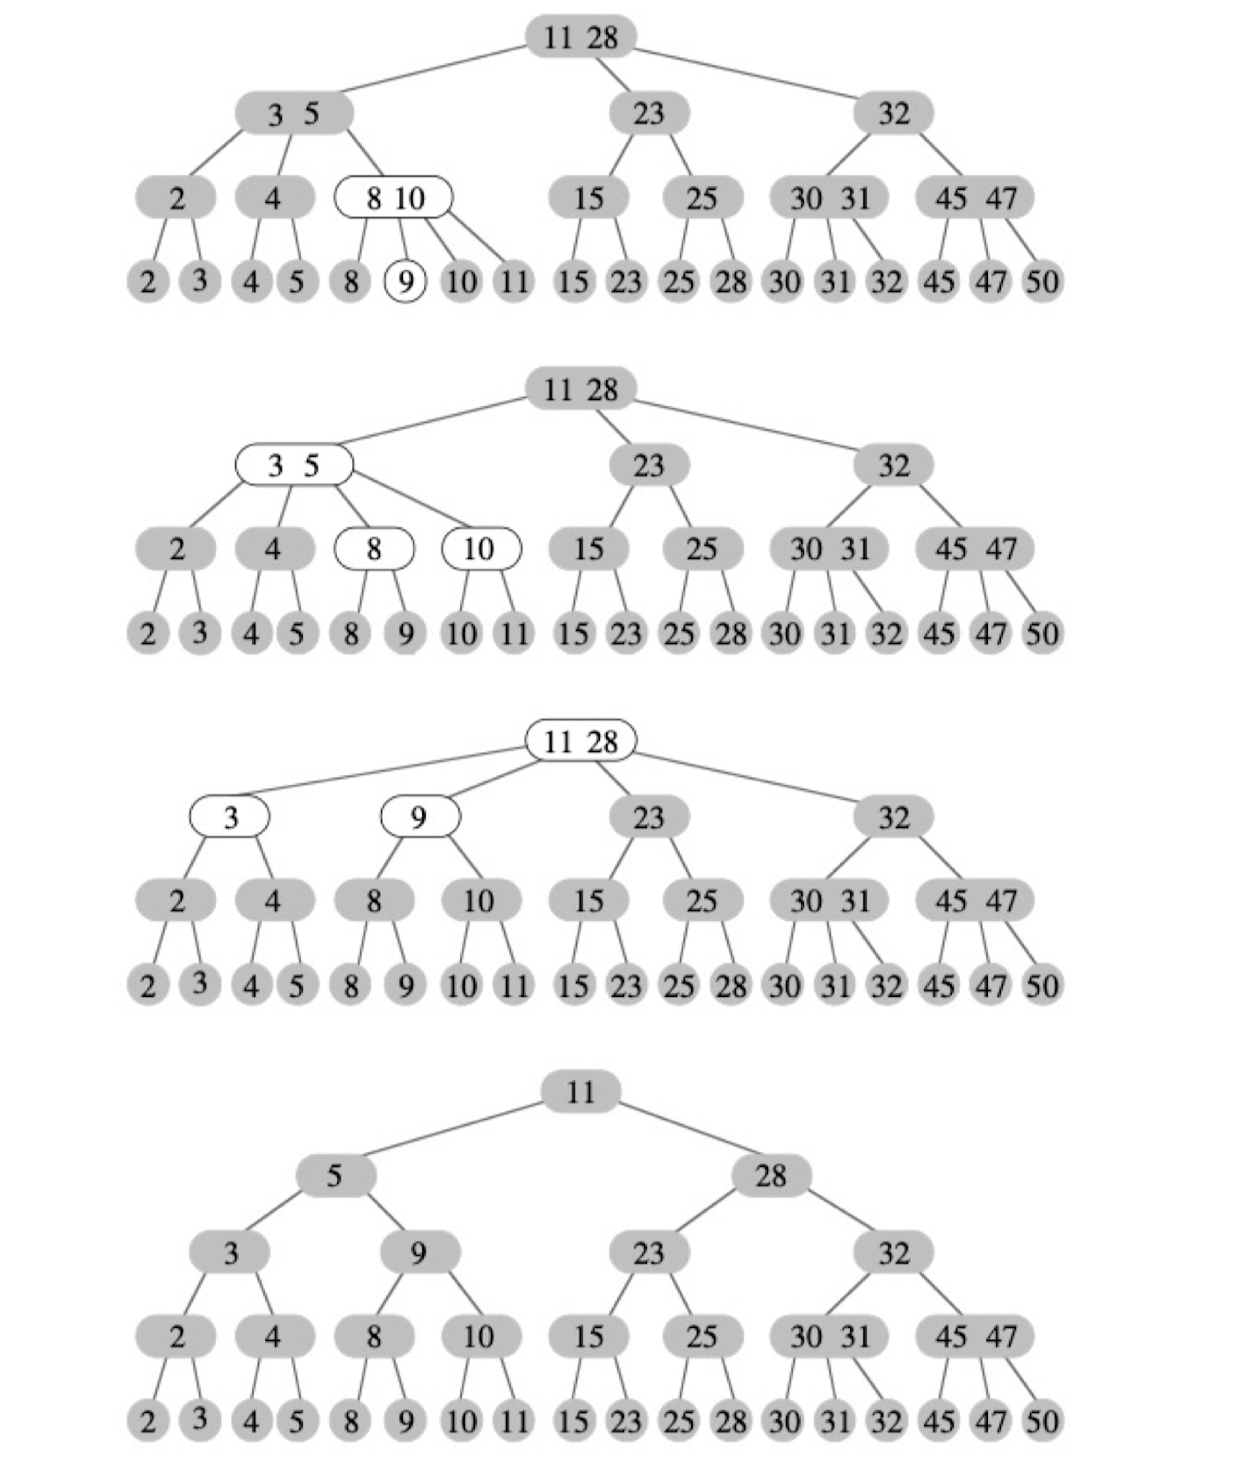
\includegraphics[width=\textwidth]{albero_2-3_split.png}
\end{figure}
\clearpage
\subsubsection{Costo operazioni}
\begin{itemize}
    \item \textbf{Ricerca}: $O(\log n)$
    \item \textbf{Inserimento}: $O(\log n)$
    \item \textbf{Cancellazione}: $O(\log n)$
\end{itemize}
Come gli alberi AVL.
\subsection{B-Alberi}
Sono un modello nato per rappresentare gli indici delle basi di dati, quando i 
dati sono troppo grandi per stare in memoria centrale. L'obiettivo non è più 
quello di fare l'albero più basso possibile, ma quello di fare il minor numero possibile di 
accessi al disco. A differenza degli alberi 2-3 le informazioni non sono solo nelle foglie
ma anche nei nodi interni.
Diamo una definizione formale di \emph{B-albero} di ordine $t$ (dove $t$) è il grado minimo:
\begin{itemize}
    \item Ogni nodo interno ha al massimo $2t$ figli 
    \item Ogni nodo interno diverso dalla radice ha almeno $t$ figli 
    \item La radice ha almeno 2 figli
    \item Tutte le foglie hanno la stessa profondità 
    \item Ogni foglia contiene $k$ chiavi ordinate dove $t - 1 \le k \le 2t - 1$
    \item Ogni nodo interno con $k + 1$ figli e sottoalberi $T_0...T_k$ contiene 
    $k$ chiavi ordinate tali che per ogni chiave $c_i$ nell'albero $T_i$ (con $i=0...k$) si ha:
    \begin{center}
        $c_0 \le a_1 \le c_1 \le a_2 \le ... \le a_{k-1} \le c_{k-1} \le a_k \le c_k$
    \end{center}
\end{itemize}
\noindent \textbf{Numero minimo di chiavi in un albero di altezza $h$}: $2t^{h}-1$\\
\textbf{Altezza massima $n$ chiavi}: $2t^{h}-1$\\
\textbf{Passi totali ricerca}: $\Theta(h \cdot \log t)$\\

\subsubsection*{Costo operazioni}

\begin{tabular}{|l|c|c|}
    \hline
    \space & \textbf{Passi di calcolo(tempo)} & \textbf{Accessi a memoria di massa}\\
    \hline
    \textbf{Ricerca} & $\Theta(\log n)$ & $\log_t n$\\
    \hline
    \textbf{Inserimento} & $\Theta(t \cdot \log n)$ & $c \cdot \log_t n$\\
    \hline
    \textbf{Cancellazione} & $\Theta(t \cdot \log n)$ & $c \cdot \log_t n$\\
    \hline
\end{tabular}
\begin{itemize}
    \item $n$ = numero di chiavi
    \item $c$ = costante piccola (dipende dall'implementazione, di solito è circa 4)
\end{itemize}

\clearpage



\section{Heapsort}
HeapSort è un algoritmo di ordinamento che utilizza la struttura dati \emph{heap}.
Vedremo innanzitutto in cosa consiste uno heap, per poi trattare l'algoritmo e la sua 
complessità in termini di numero di confronti. Vedremo poi come uno heap possa
essere rappresentato nell'array stesso da ordinare, in modo tale da avere un implementazione in loco.

\subsection{La struttura dati \emph{Heap}}
Uno \emph{heap} è un \emph{albero binario quasi completo}, ovvero completo almeno
fino al penultimo livello, tale che la chiave contenuta in ogni suo nodo è maggiore 
o uguale alla chiave contenuta nei figli.\\
Poichè un albero binario di altezza $h$ contiene $2^{h+1} - 1$ nodi,
possiamo affermare che in uno heap di altezza $h$ il numero $n$ di nodi soddisfa $2^h \le n \le 2^{h + 1}$, da cui otteniamo
$h \le \log_2 n \le h + 1$ e dunque $h = \lfloor \log_2 n \rfloor$.\\
\begin{wrapfigure}{r}{7cm}
    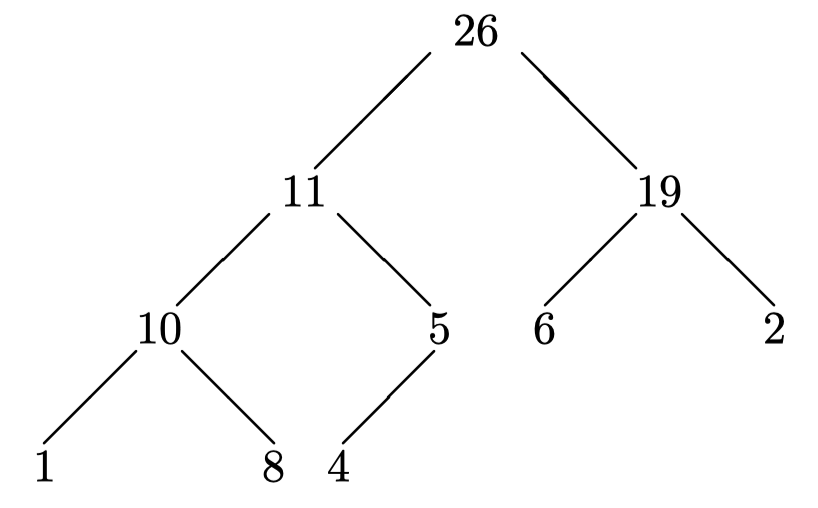
\includegraphics[scale = 0.5]{heap.png}
\end{wrapfigure}
La radice di uno heap contiene sempre la chiave maggiore. Pertanto, disponendo di 
uno heap contente le chiavi che dobbiamo ordinare, possiamo prelevare l'elemento che si trova
nella radice e collocarlo, come unico elemento, nella sequenza ordinata che dobbiamo
produrre come risultato, che costruiremo a partire dal fondo. Una volta fatto ciò possiamo
modificare la struttura in modo da riottenere uno heap ed applicare lo stesso procedimento.
\subsection{Sistemare uno heap}
Per risistemare uno heap applichiamo la seguente strategia.\\
Sostituiamo la chiave contenuta nella radice con quella contenuta nell'ultima
delle foglie, cioè quella che si trova più a destra nell'ultimo livello, rimuovendo
tale foglia. Tutti i nodi rispettano la condizione di heap, tranne la radice che potrebbe contenere 
una chiave inferiore rispetto a uno o entrambi i figli. In questo caso facciamo "scendere"
il dato presente nella radice, scambiandolo con quello di chiave maggiore tra i figli.
Se la condizione di heap non è rispettata dal figlio in cui abbiamo spostato il dato, 
iteriamo lo stesso procedimento su di esso.
\clearpage
\begin{figure}[h]
    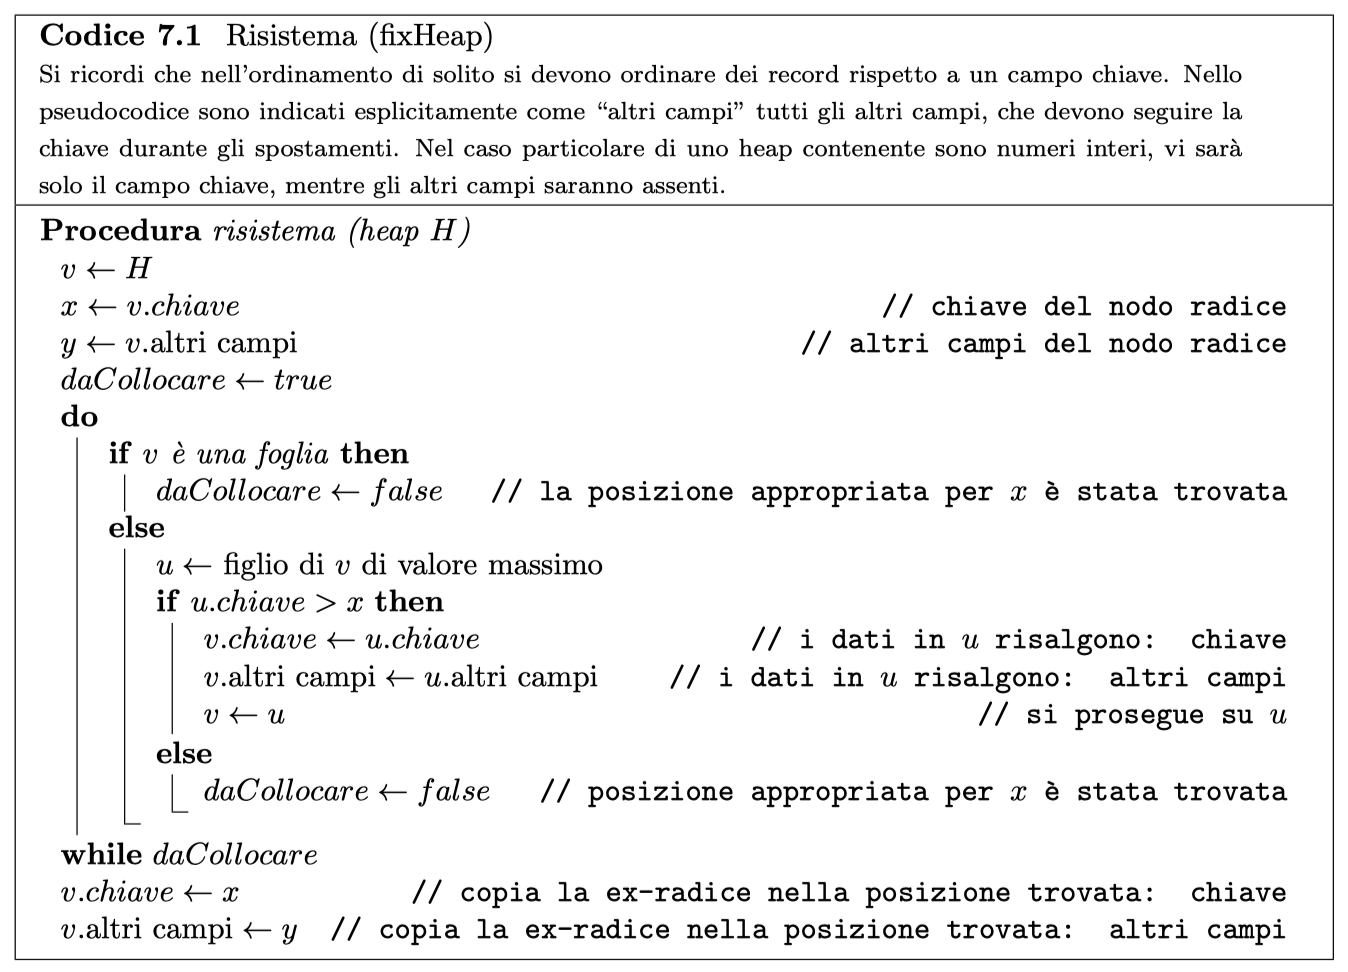
\includegraphics[width=\textwidth]{risistema.png}
\end{figure}
\subsubsection*{Numero di confronti}
Il numero di confronti usato da \texttt{risistema}, nel caso peggiore, $\Theta(h)$,
dove $h$ è l'altezza dello heap. Infatti il valore presente nella radice viene fatto scendere
lungo un cammino fino a raggiungere la posizione corretta che, nel caso peggiore,
potrebbe essere una foglia a distanza massima dalla radice. In questo processo, ad ogni passo viene
ispezionato un nodo lungo il cammino, determinando la chiave massima tra i figli e 
confrontandola con la chiave ispezionata. Pertanto per ogni nodo del cammino ho 2 confronti.
\clearpage

\subsection{Creazione di uno heap}
Supponiamo di disponere di un albero binario quasi completo le cui chiavi non rispettino però
la condizione di heap. Studieremo due soluzioni per trasformarlo in uno heap. La seconda soluzione è meno dispendiosa in 
termini di memoria.
\subsubsection*{Soluzione ricorsiva}
Strategia \emph{divide-et-impera}:
\begin{itemize}
    \item Se l'albero è vuoto non devo fare nulla
    \item Se l'albero non è vuoto trasformiamo ricorsivamente ciascuno dei due 
    sottoalberi sinistro e destro in heap; a questo punto tutti i nodi, eccetto la radice,
    soddisfano la condizione di heap. Applicando la procedura \texttt{risistema} possiamo trasformare l'albero in uno heap
\end{itemize}
\begin{figure}[h]
    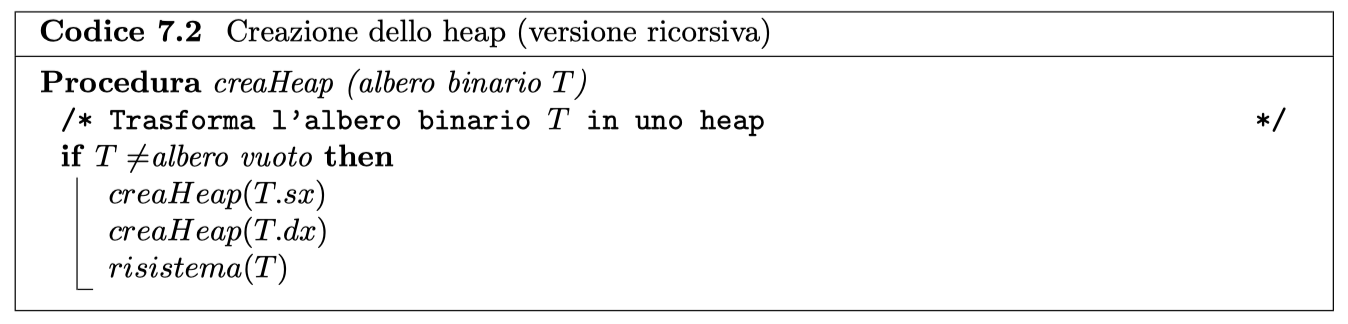
\includegraphics[width=\textwidth]{crea_heap_ricorsivo.png}
\end{figure}

\subsubsection*{Soluzione iterativa}
Anzichè costruire lo heap in maniera top-down, possiamo procedere in maniera bottom-up partendo
dalle foglie dell'albero. Ispezioniamo cioè l'albero a partire dall'ultima foglia, trasformando ogni sottoalbero
in uno heap. Quindi:
\begin{itemize}
    \item Iniziamo a considerare ciascun nodo di profondità $h$, da destra verso sinistra,
    e trasformiamo in heap il sottoalbero che ha tale nodo come radice (questi nodi sono foglie, quindi 
    i relativi sottoalberi sono già heap e per essi non occorre fare nulla).
    \item Passiamo a considerare ciascun nodo di profondità $h - 1$ (sempre da destra verso sinistra)
    e trasformiamo in heap il sottoalbero che ha radice in esso.
    \item Ripetiamo lo stesso procedimento considerando man mano profondità inferiori
    sino ad arrivare alla radice. A questo punto l'intero albero è uno heap.
\end{itemize}

\noindent Poichè i sottoalberi sono trasformati in heap a partire dal basso, quando in questo procedimento dobbiamo
trasformare in heap il sottoalbero $T_{x}$ che ha come radice un nodo $x$ di profondità $p$, i sottoalberi di $x$, avendo profondità
$p-1$, sono già stati trasformati in heap in passi precedenti. Dunque l'unico nodo di $T_{x}$ che potrebbe non
rispettare la condizione di heap è radice $x$. Quindi è sufficiente applicare \texttt{risistema}
per trasformare $T_{x}$ in uno heap.
\begin{figure}[h]
    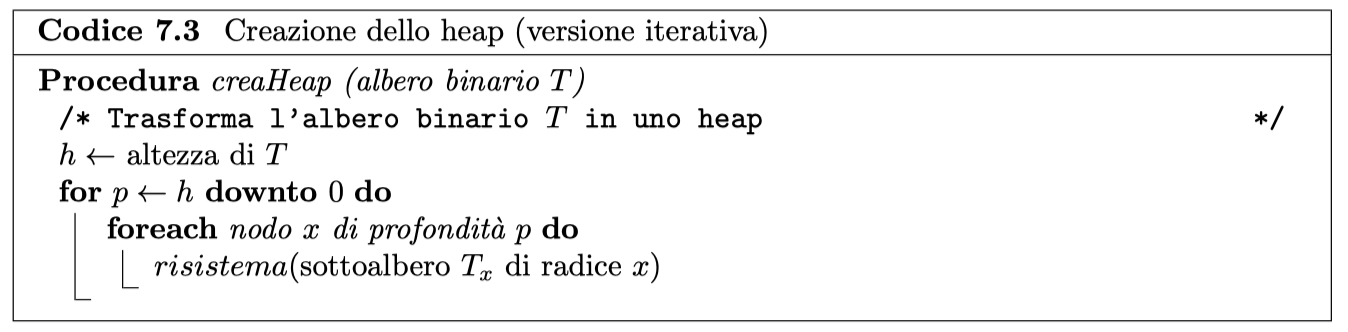
\includegraphics[width=\textwidth]{crea_heap_iterativo.png}
\end{figure}

\subsubsection*{Numero di confronti}
\texttt{creaHeap} chiama \texttt{risitema} un certo numero di volte, per sottoalberi di altezze differenti.
Il numero di confronti per trasformare in heap tutti i sottoalberi di profondità $p$ è 
$\Theta(h-p)2^p$. Nel ciclo esterno $p$ varia su tutte le profondità, cioè da 0 ad $h$.
Sommando su di esse otteniamo che il numero di confronti è $2^{h+1} - 2 - h$.\\
Essendo l'albero completo la sua altezza è logaritmica rispetto al numero di nodi. Questo 
permette di concludere che il numero di confronti di \texttt{creaHeap} è $\Theta(n)$, cioè lineare 
rispetto al numero di chiavi.

\subsection{Schema di \texttt{heapSort}}
\begin{figure}[h]
    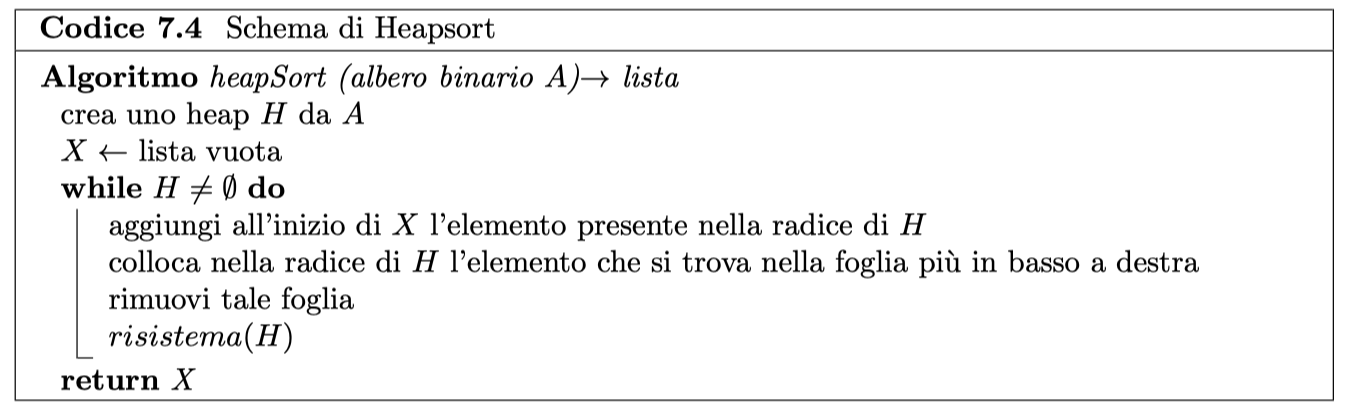
\includegraphics[width=\textwidth]{schema_heapsort.png}
\end{figure}

\subsubsection*{Numero di confronti}
\texttt{creaHeap} effettua $\Theta(n)$ confronti. Segue poi la parte iterativa in cui,
ad ogni passo, si preleva la radice e si risistema lo heap. Queste operazioni vengono ripetute
fino a svuotare lo heap, quindi $n$ volte. Risistemare lo heap utilizza, nel caso peggiore, un numero
di confronti proporzionale alla sua altezza, che è logaritmica. Dunque il numero
di confronti, nel caso peggiore, è $\Theta(n\log n)$.
\clearpage

\subsection{Ordinamento in loco di array tramite \texttt{heapSort}}
Si può implementare l'algoritmo in modo semplice senza ricorrere a strutture aggiuntive, servendosi
di una corrispondenza tra alberi binari quasi completi e array. Supponiamo di disporre del seguente array:

\begin{figure}[h]
    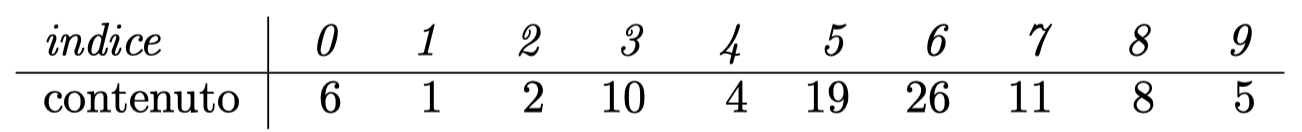
\includegraphics[width=10cm]{heap_array.png}
\end{figure}

\noindent Immaginiamo di collocare gli elementi dell'array nell'ordine in cui compaiono 
in un albero binario, riempiendo ciascun livello da sinistra verso destra a partire 
dalla radice, come in una visita in ampiezza. L'albero che otteniamo è il seguente:

\begin{figure}[h]
    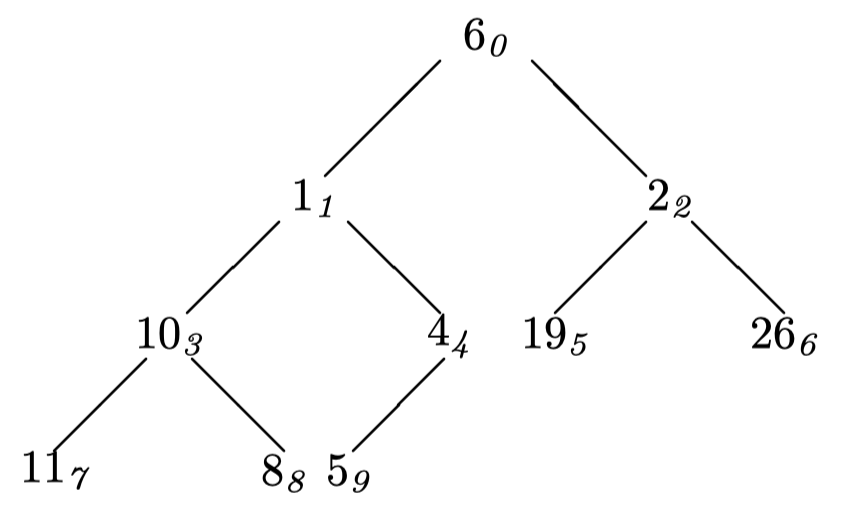
\includegraphics[width=7cm]{heap_albero_binario.png}
\end{figure}

L'albero è quasi completo, con le foglie dell'ultimo livello più a sinistra possibile.\\
Osserviamo che i figli del nodo che nell'array ha indice $i$ hanno, se esistono, indice
$2i + 1$ e $2i + 2$.\\
L'array che rappresenta un albero binario quasi completo è detto \emph{vettore posizionale}.\\
\begin{figure}[h]
    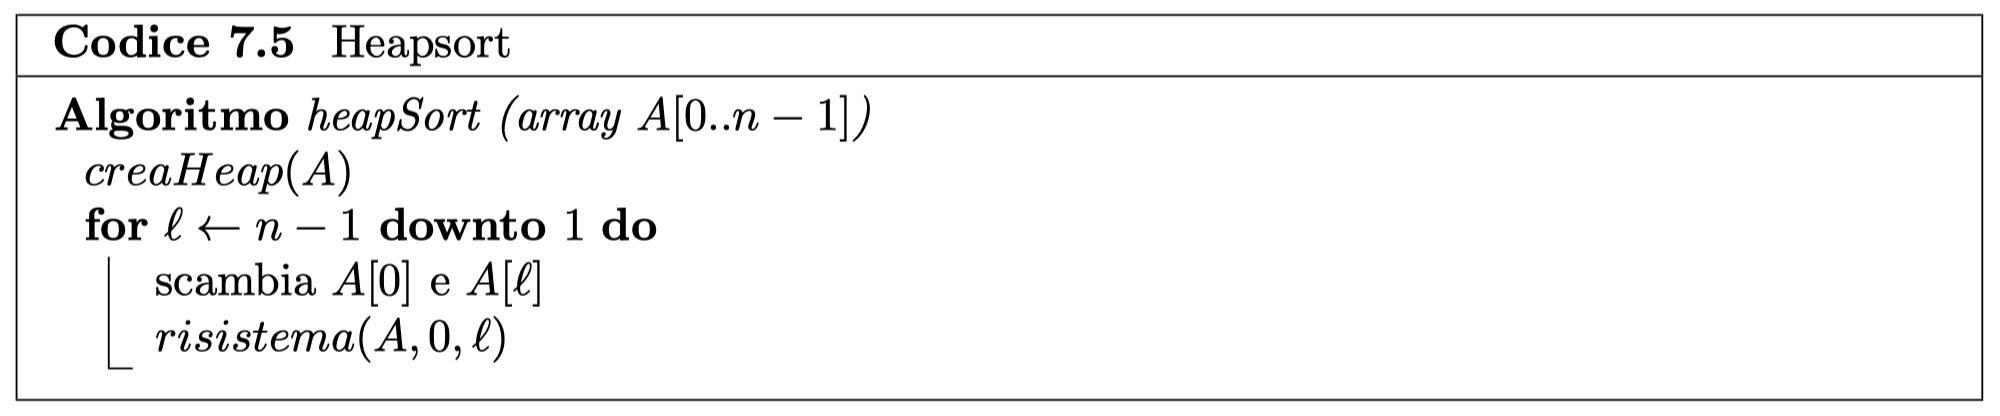
\includegraphics[width=\textwidth]{heapsort_array.png}
\end{figure}

Si possono modificare anche \texttt{creaHeap} e \texttt{risistema} affinchè lavorino
direttamente con l'array.

\begin{figure}[h]
    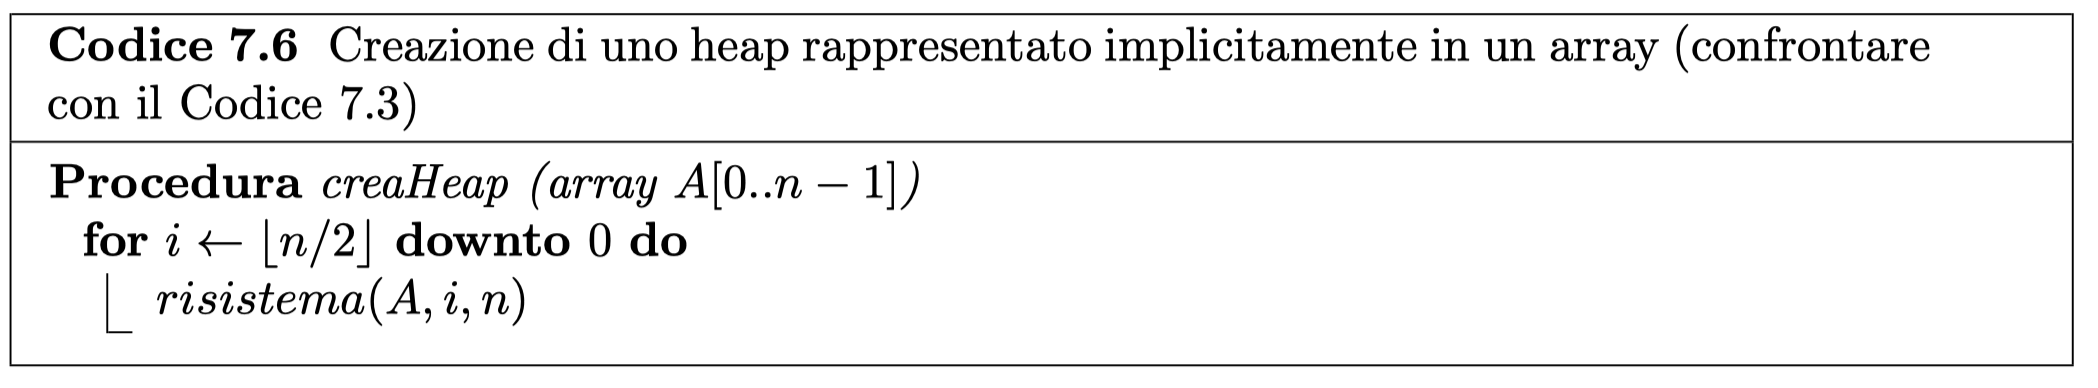
\includegraphics[width=\textwidth]{creaheap_array.png}
\end{figure}

\begin{figure}[h]
    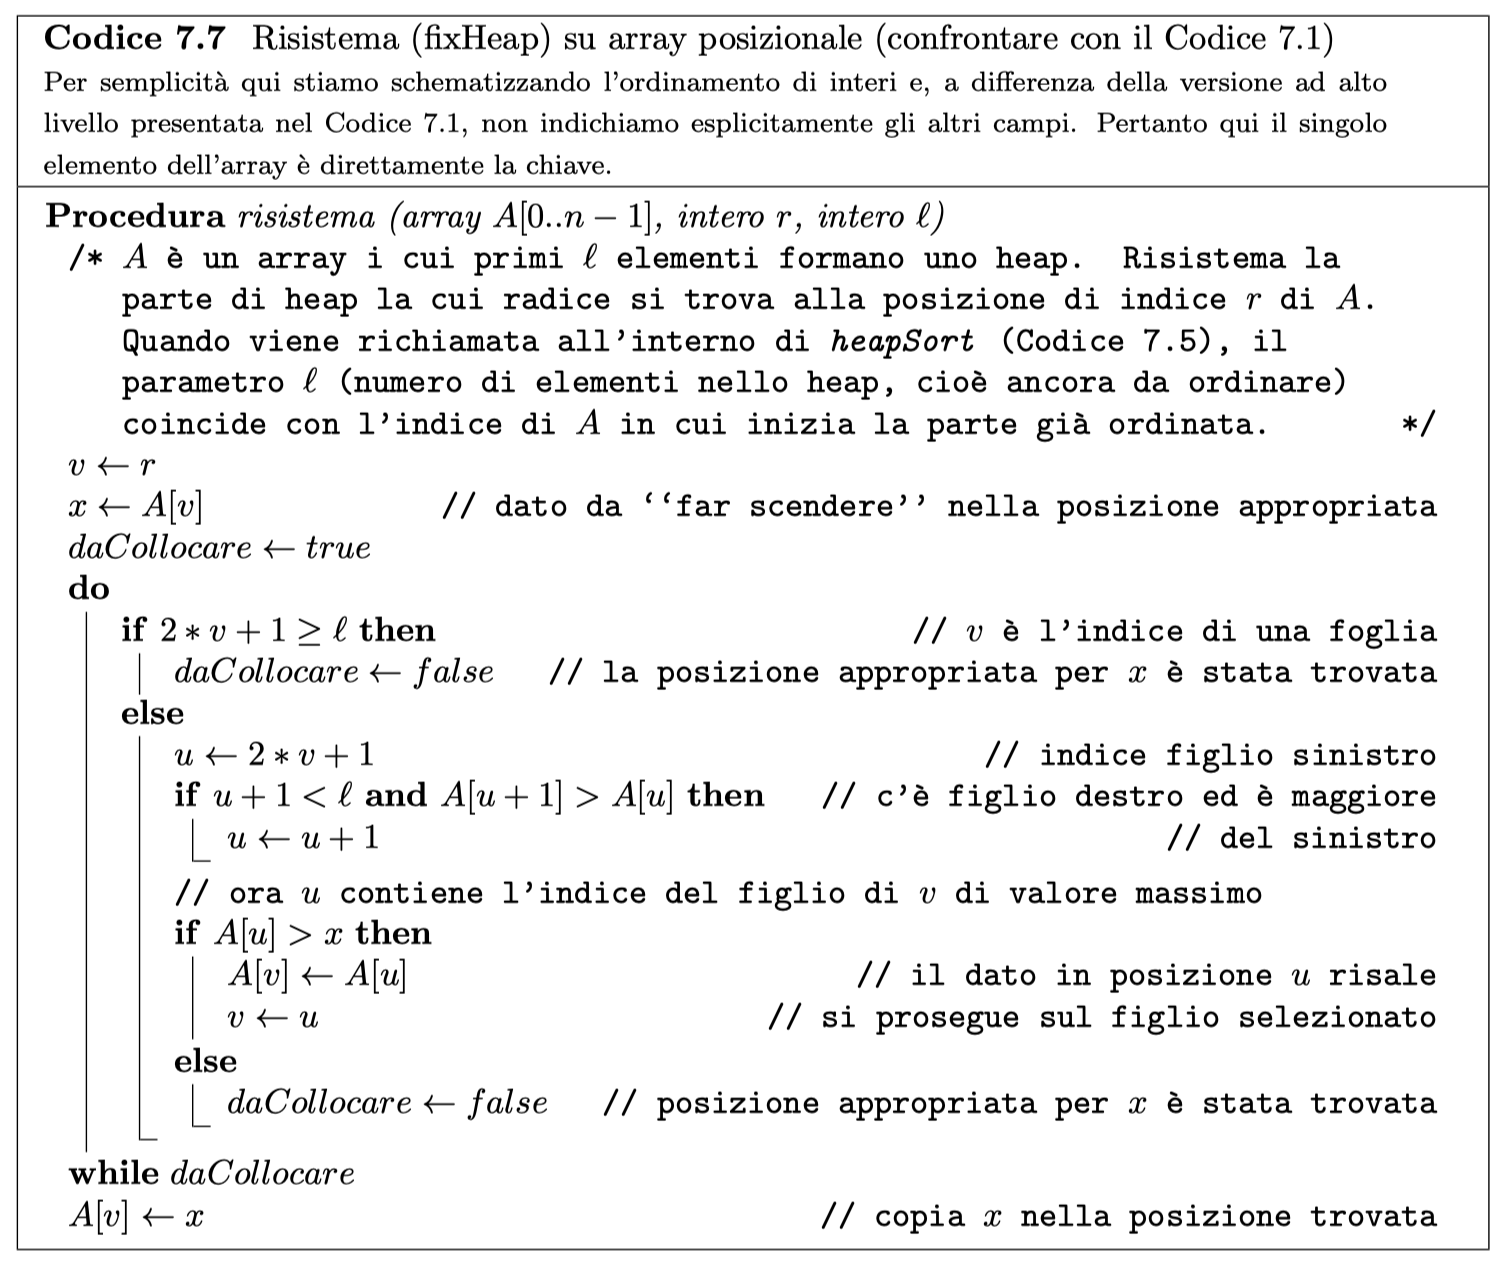
\includegraphics[width=\textwidth]{risistema_array.png}
\end{figure}
\clearpage

\subsection{Spazio}
Utilizzando la versione iterativa di \texttt{creaHeap} e l'implementazione in loco,
l'algoritmo utilizza spazio costante oltre all'array da ordinare.

\subsection{Costo operazioni su heap}
\begin{itemize}
    \item Trovare elemento di chiave massima $\rightarrow$ $O(1)$ passi
    \item Cancellare elemento di chiave massima $\rightarrow$ $\Theta(\log 1)$ passi
    \item Inserire un nuovo elemento $\rightarrow$ $\Theta(\log n)$ passi
    \item Cancellare elemento di chiave $x$ $\rightarrow$ $\Theta(\log n)$ passi
    \item Modificare la chiave di un elemento $\rightarrow$ $\Theta(\log n)$ passi
\end{itemize}

\subsection{Riassumendo}
\texttt{HeapSort} è un algoritmo di ordinamento in loco che, per ordinare $n$ elementi 
effettua $\Theta(n \log n)$ confronti. Pertanto, se ciascun confronto viene effettuato
in tempo $O(1)$, il tempo complessivo è $\Theta(n \log n)$.\\
Si può verificare che questo metodo non è stabile.
\clearpage
\section{Riassunto ordinamento}
Il \emph{problema dell'ordinamento} può essere definito in questo modo:

\noindent \textbf{Input}: $n$ elementi $x_1, x_2, ... , x_n$ appartenenti a un dominio $D$ su cui
è definita una relazione $\le$ di \emph{ordine totale}.\\[15pt]
\textbf{Output}: Sequenza $x_{j1}, x_{j2}, ..., x_{jn}$ dove ($j_1...j_n$) 
è una permutazione di (1, 2, ... $n$) tale che\\ $x_{j1} \le ... \le x_{jn}$.

\begin{figure}[h]
    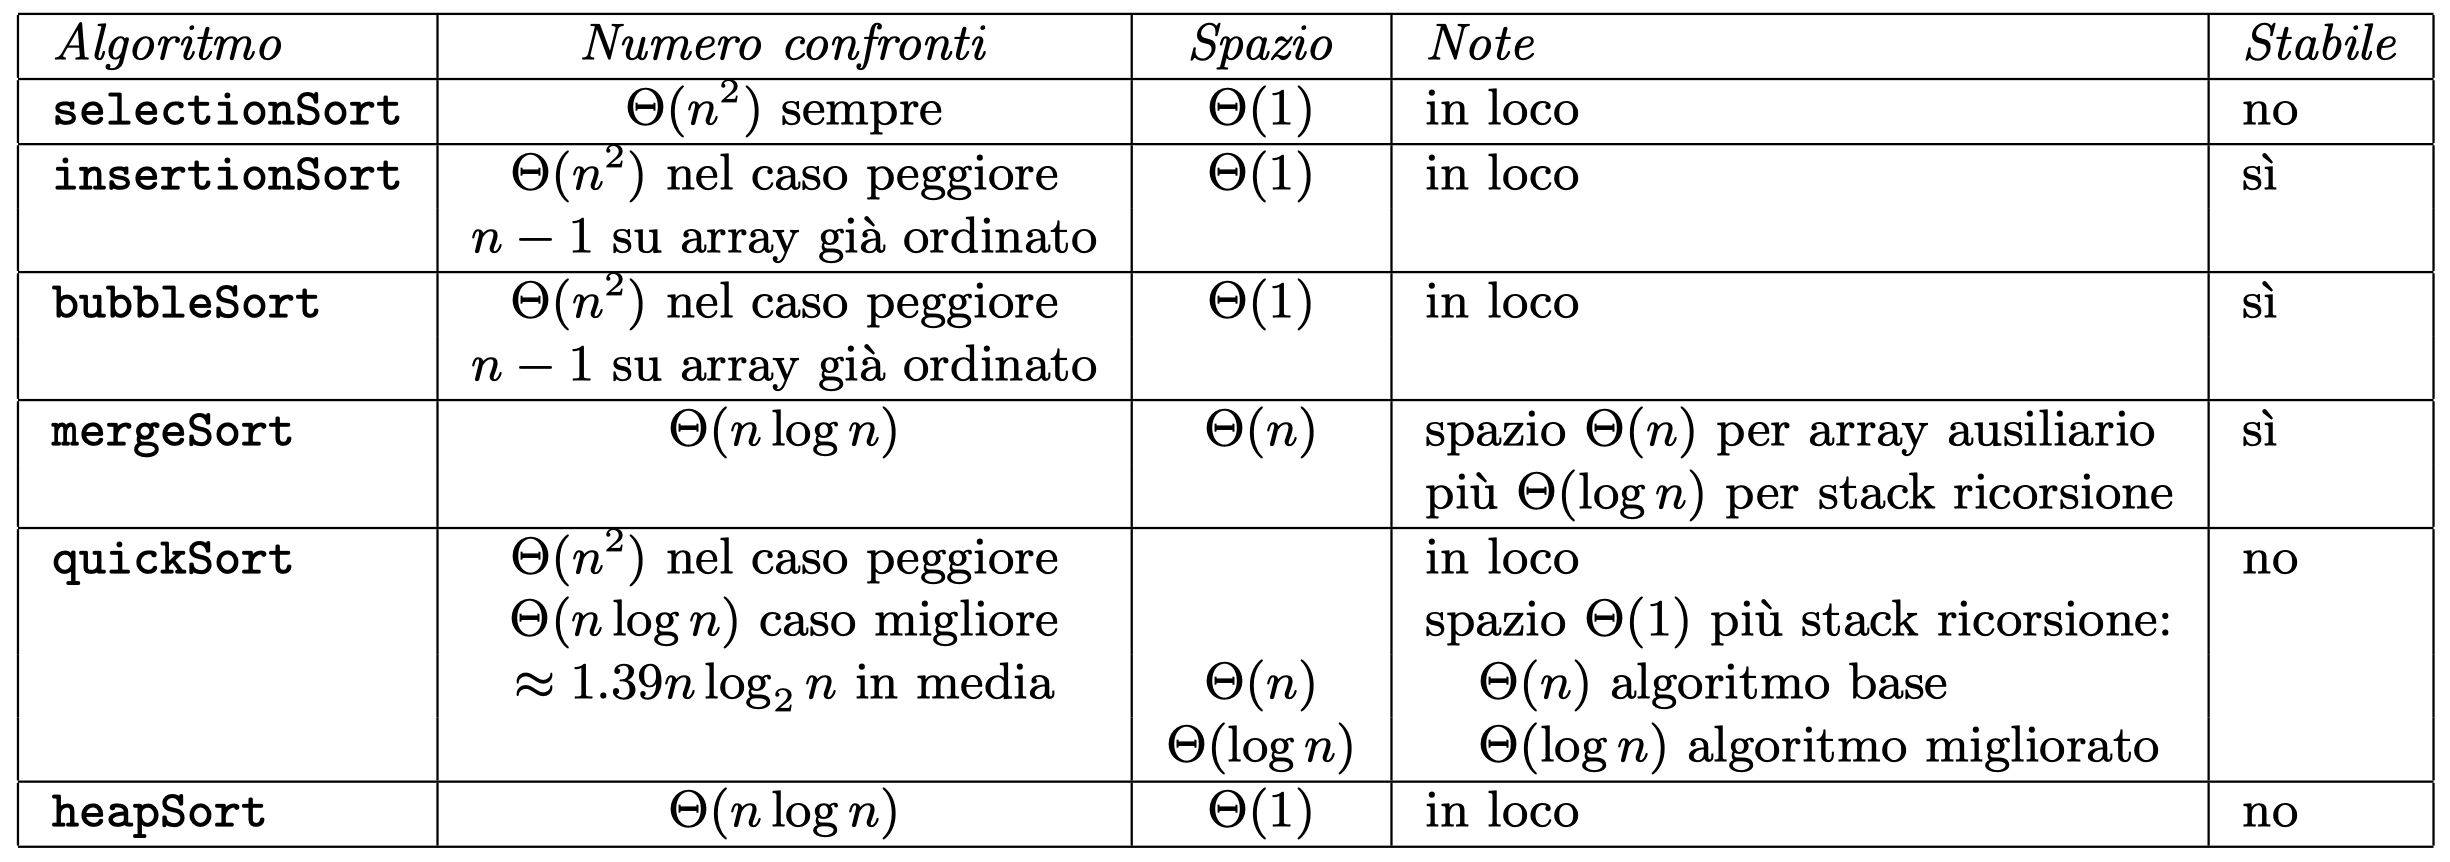
\includegraphics[width=\textwidth]{riepilogo_ordinamento.png}
\end{figure}


\subsection{Numero minimo di confronti}
Dimostreremo ora che qualsiasi algoritmo di ordinamento basato su confronti 
richiede, nel caso peggiore, un numero di confronti almeno dell'ordine di $n \log n$.
Le possibili computazioni di un algoritmo di ordinamento su sequenze di $n$ elementi 
possono essere rappresentate mediante un \emph{albero di decisione}, cioè un albero
binario in cui ciascun nodo interno rappresenta un operazione di confronto, con associati due 
sottoalberi, che dipendono dall'esito di tale operazione, mentre ogni foglia rappresenta 
una risposta dell'algoritmo, cioè un possibile ordine tra le chiavi.

\begin{center}
    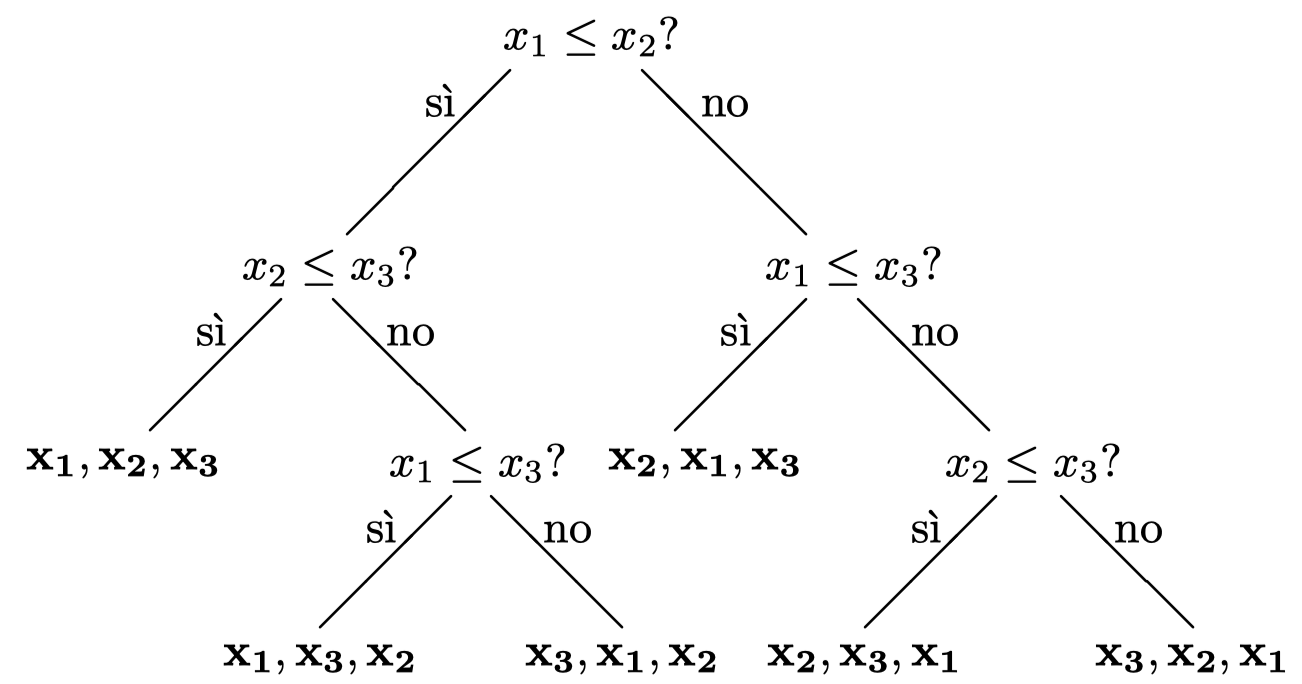
\includegraphics[scale = 0.4]{albero_decisione.png}
\end{center}
\clearpage
\noindent Indipendentemente dalla strategia utilizzata per eseguire i confronti, l'albero dovrà avere un
numero di foglie pari almeno al numero dei possibili ordini tra le chiavi, cioè
al numero di possibili permutazioni di $n$ elementi, che è $n!$. Il numero massimo
di confronti utilizzato da una strategia è pari alla profondità dell'albero.
Si può verificare che la profondità di un albero binario con $k$ foglie è
almeno logaritmica in $k$.\\
Per trovare il numero di confronti necessari nel caso peggiore stimiamo quindi 
la profondità minima che deve avere un albero con $n!$ foglie, calcolando il logaritmo di $n!$.
Utilizzando l'approssimazione di Stirling $n! \approx \sqrt{2 \pi n (\frac{n}{e})^n}$ si ottiene $\Theta(n \log n)$.\\
Possiamo concludere che \emph{ogni} algoritmo di ordinamento basato su confronti richiede nel caso peggiore 
un numero di confronti tra chiavi dell'ordine di $n \log n$ per ordinare $n$ elementi.
\clearpage

\input{sections/19-code_priorità.tex}
\section[Ordinamento senza confronti]{Algoritmi di ordinamento non basati su confronti}
\subsection{IntegerSort}
È un algoritmo di ordinamento che si basa sulla conoscenza a priori dell'intervallo in cui sono compresi i valori da ordinare.
L'algoritmo conta il numero di occorrenze di ciascun valore presente nell'array 
da ordinare, memorizzando questa informazione in un array temporaneo di dimensione
pari all'intervallo di valori. Il numero di ripetizioni dei valori indica
la posizione del valore immediatamente successivo. 
\begin{itemize}
    \item Si calcolano il valore massimo e il valore minimo, $max(A)$ e $min(A)$
    \item Si prepara un array ausiliario $C$ di dimensione pari all'intervallo 
    di valori con entrate $C[i]$ che rappresentano la frequenza dell'elemento
    $i + min(A)$
    \item Si visita l'array $A$ aumentando l'elemento di $C$ corrispondente.
    \item Si visita l'array $C$ in ordine e si scrivono su $A$ $C[i]$ copie del valore $i + min(A)$ 
\end{itemize}

\subsubsection*{Complessità}
L'algoritmo esegue 3 iterazioni, 2 di lunghezza $n$ per individuare massimo e minimo e per il calcolo delle
occorrenze dei valori, e una di lunghezza $k = (max(A)- min(A) - 1)$.\\
La complessità totale è quindi $O(n+k)$. \\
Conviene utilizzarlo quando il valore di $k$ è $O(n)$.

\begin{figure}[h]
    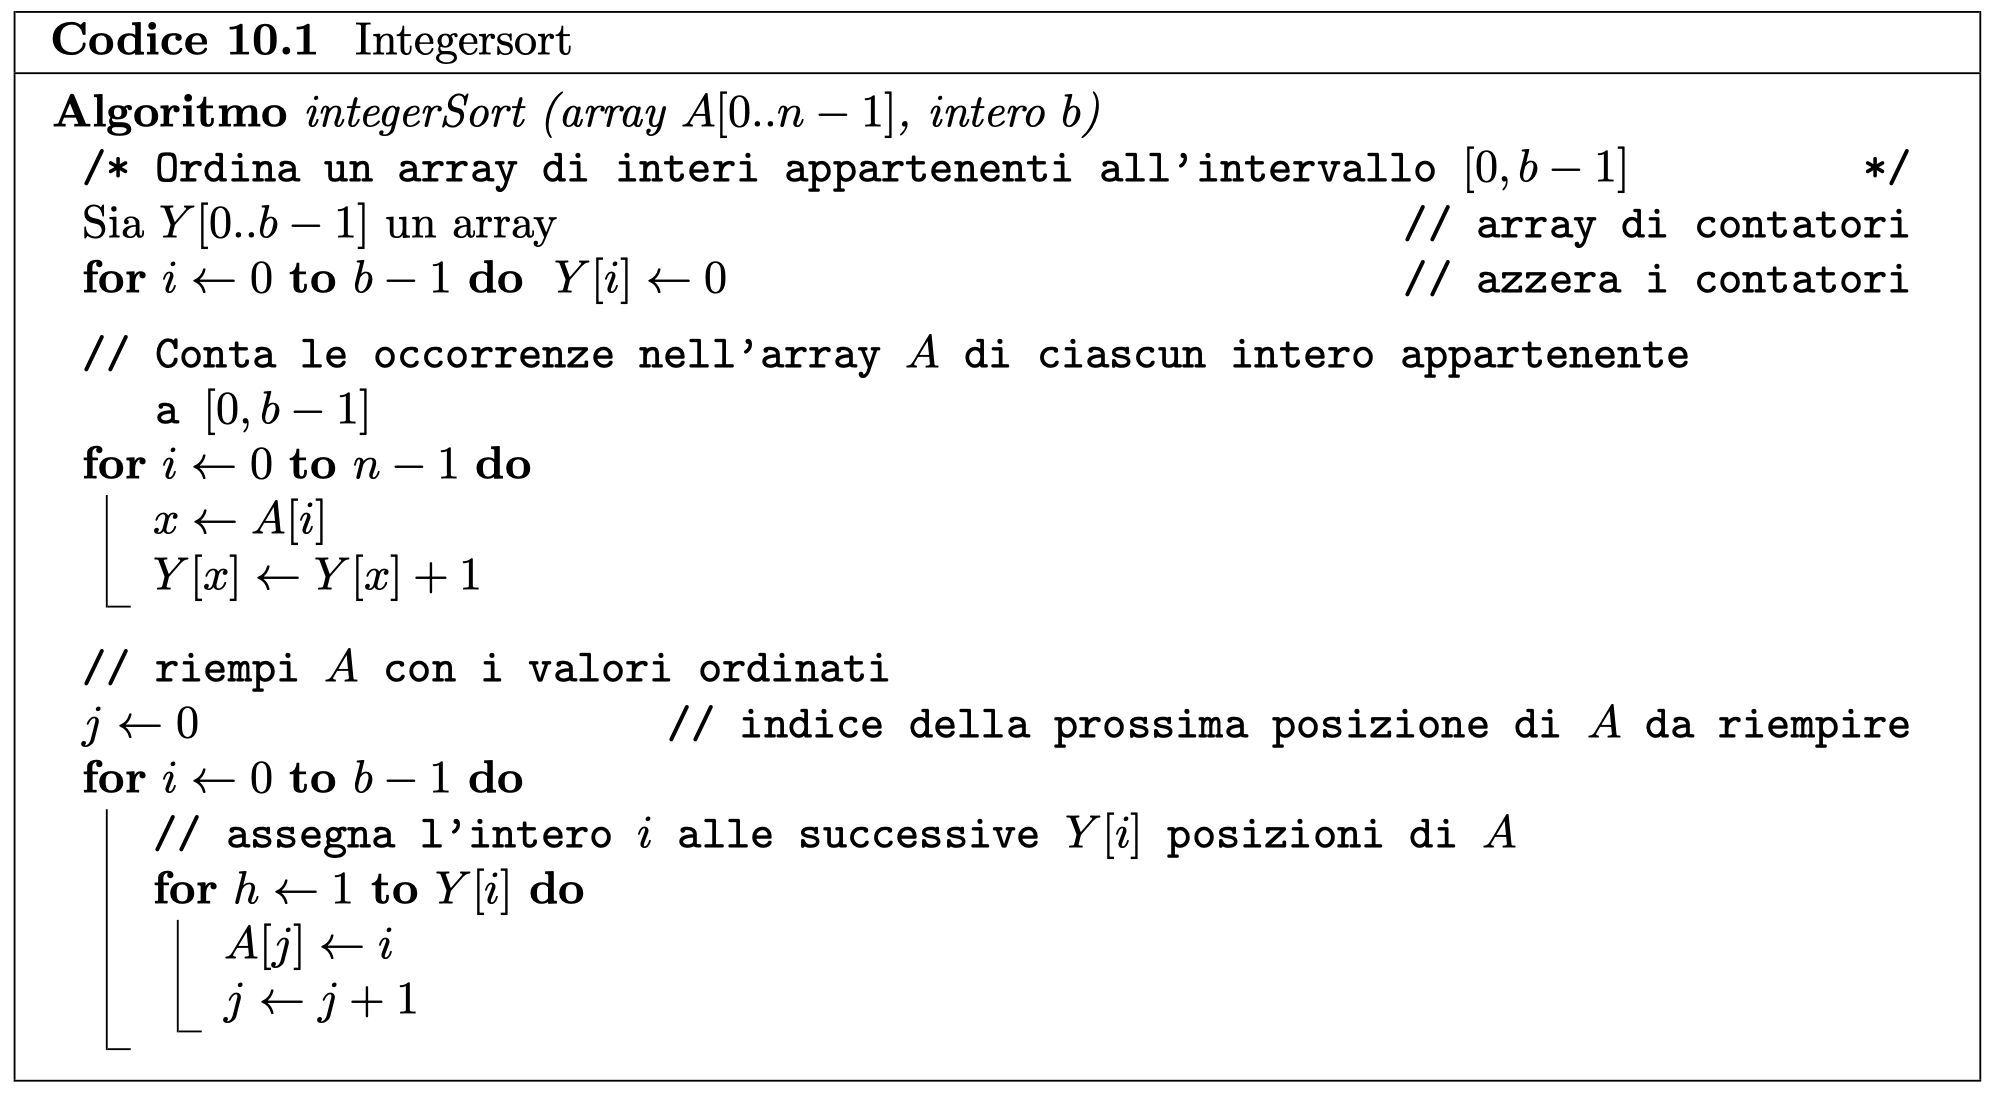
\includegraphics[width=\textwidth]{integerSort.png}
\end{figure}
\clearpage

\subsection{BucketSort}

\begin{wrapfigure}{r}{7cm}
    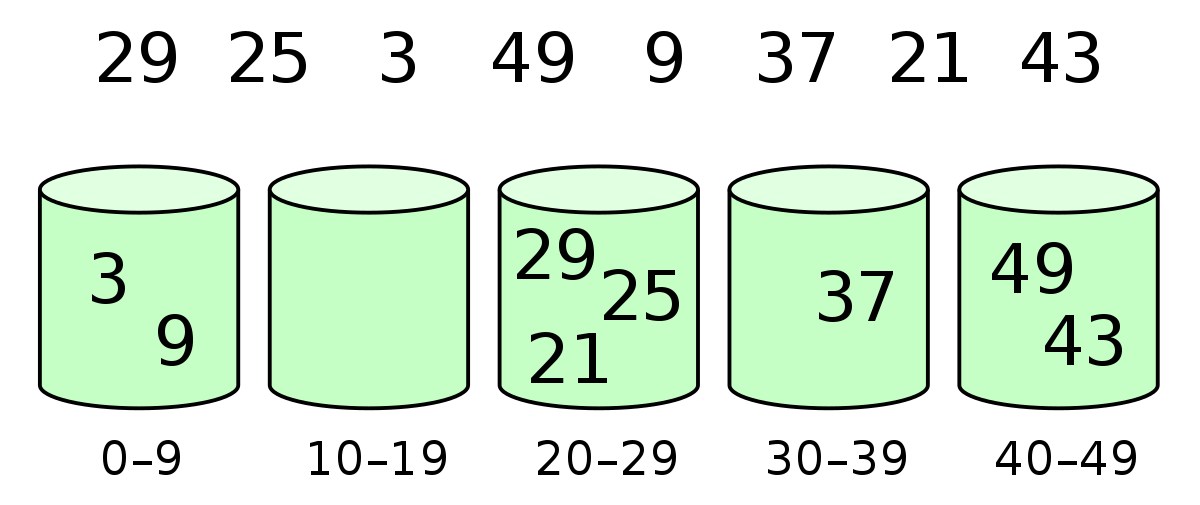
\includegraphics[scale = 0.2]{bucketsort_es.png}
\end{wrapfigure}

È un algoritmo di ordinamento per valori numerici che si assume siano distribuiti
uniformemente in un intervallo $[0,1)$\\
Se $n$ è il numero di elementi da ordinare, l'intervallo $[0,1)$ è diviso in $n$
intervalli di uguale lunghezza, detti \emph{bucket}.
Ciascun valore dell'array è quindi inserito nel bucket a cui appartiene, i valori
all'interno di ogni bucket vengono ordinati e l'algoritmo di conclude con la concatenazione
dei valori contenuti nei bucket.

\subsubsection*{Complessità}
La complessità di \texttt{bucketSort} è $O(n)$ per tutti i cicli, a parte l'ordinamento dei 
singoli bucket. Date le premesse sull'input, utilizzando \texttt{insertionSort}
l'ordinamento di ogni bucket è $\Theta(1)$, quindi la complessità media è
$O(n)$ per tutto l'algoritmo. La complessità complessiva nel caso migliore è 
$O(n+m)$ dove $m$ è il massimo valore nell'array.

\begin{figure}[h]
    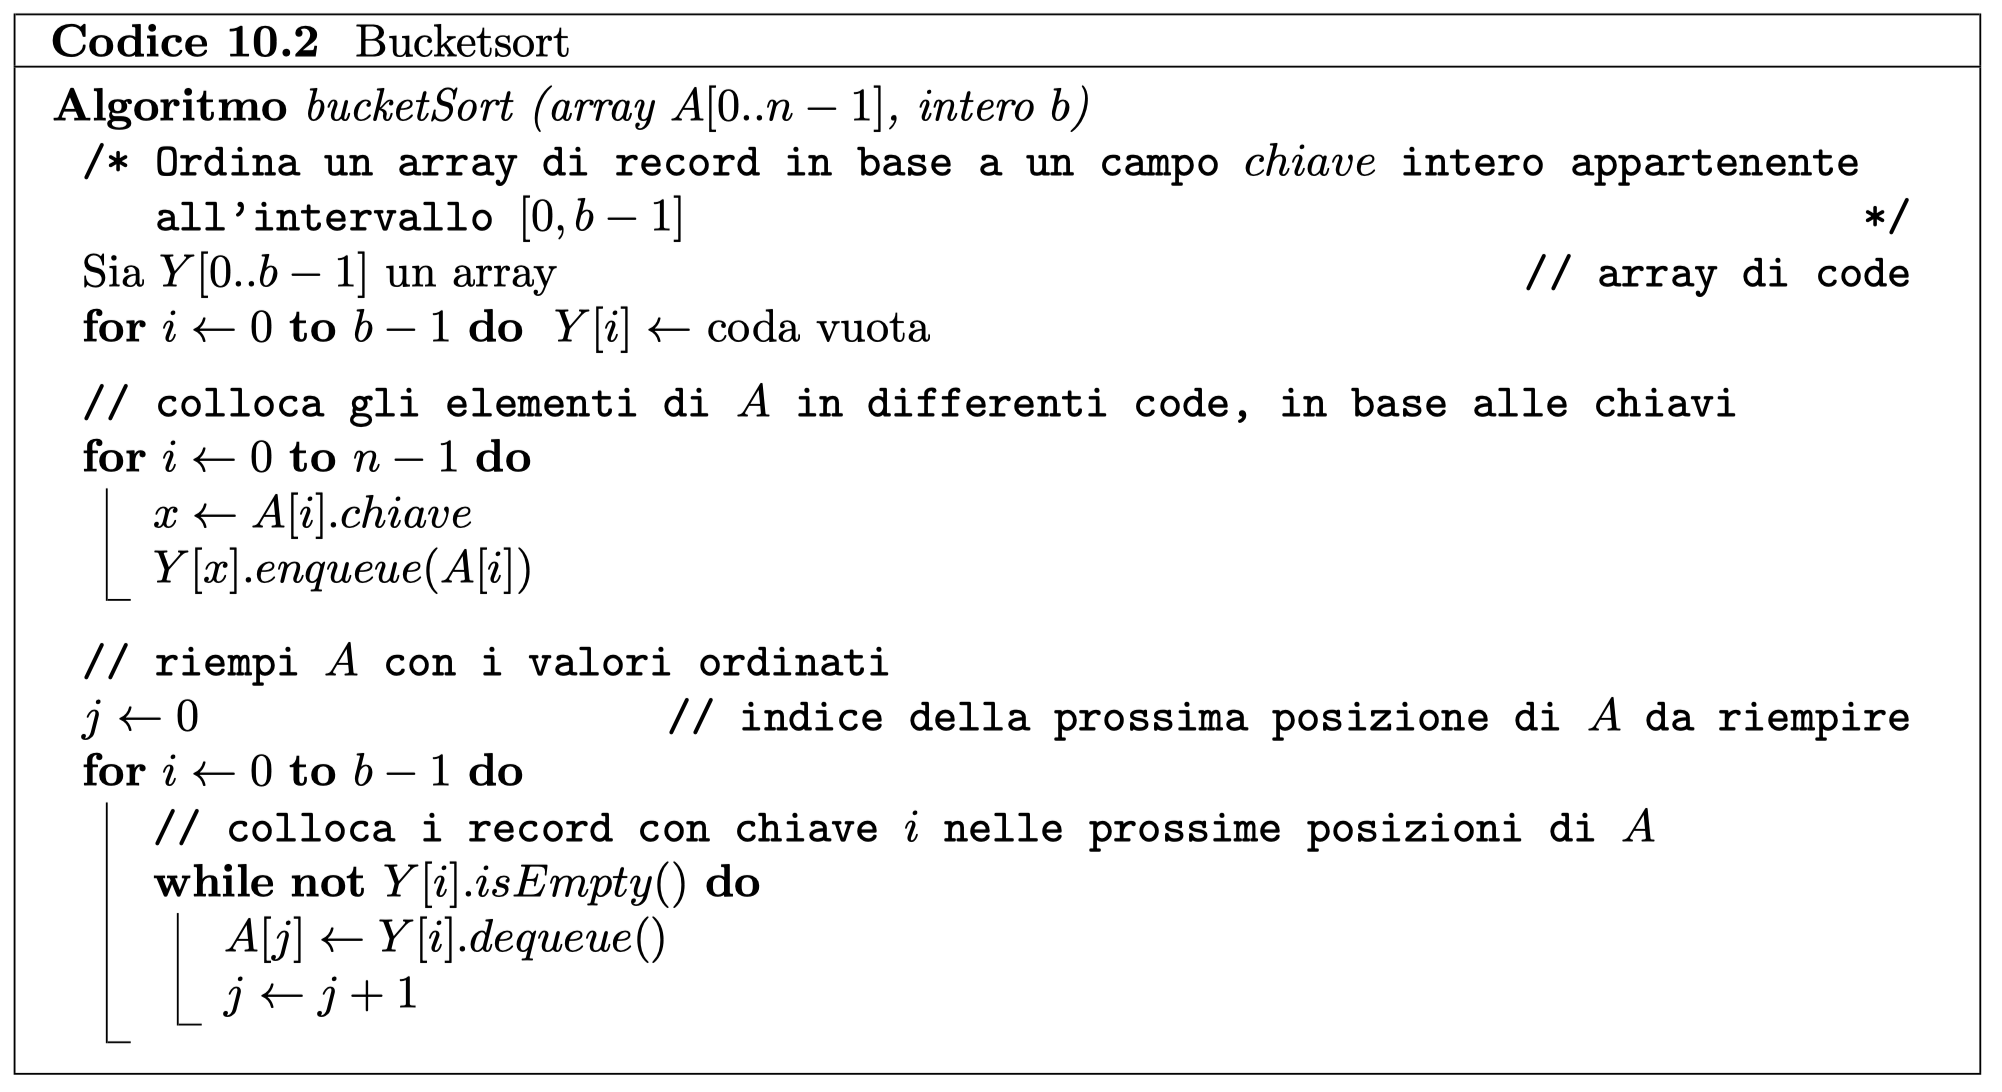
\includegraphics[width=\textwidth]{bucketSort.png}
\end{figure}
\clearpage
\subsection{RadixSort}
È un algoritmo che esegue degli ordinamenti per posizione della cifra, partendo 
dalla cifra meno significativa. Questo affinchè l'algoritmo non si trovi a dovere
operare ricorsivamente su sottoproblemi di dimensione non valutabile a priori.

\begin{wrapfigure}{r}{7cm}
    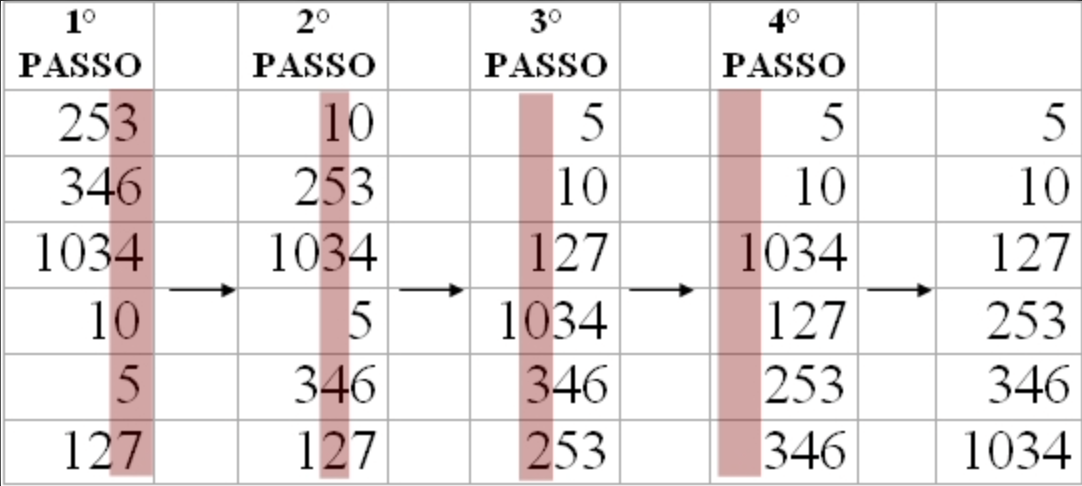
\includegraphics[scale = 0.4]{radixsort_es.png}
\end{wrapfigure}

\subsubsection*{Complessità}
L'algoritmo ha complessità computazionale pari a $O(n\cdot k)$ dove $n$ è 
il numero di elementi da ordinare e $k$ è la media del numero di cifre degli $n$ elementi.
Se $k$ risulta essere minore di $n$ non si ha guadagno rispetto a \texttt{integerSort}
che opera in tempo lineare. Se $k > n$ l'algoritmo può risultare peggiore anche 
rispetto agli algoritmi basati su confronti.
\begin{figure}[h]
    \includegraphics[width=\textwidth]{radixSort.png}
\end{figure}
\clearpage

\section[Union-Find]{Rappresentazione di partizioni (UNION-FIND)}
Dato un insieme $\mathcal{A}$, una partizione è una famiglia di sottoinsiemi $\mathcal{A}_{1...k}$ tali che 
\begin{itemize}
    \item $\mathcal{A}_{i} \neq \emptyset$
    \item  $\mathcal{A}_{i} \cap \mathcal{A}_{j} = \emptyset$
    \item $\mathcal{A}_{1} \cup ... \cup \mathcal{A}_{k} = \mathcal{A}$
\end{itemize}

Vogliamo rappresentare una collezione di insiemi disgiunti mediante le operazioni:
\begin{itemize}
    \item \texttt{UNION(A, B)} unisce gli insiemi $A$ e $B$ in un unico insieme $A$
    \item \texttt{FIND(X)} restituisce il nome dell'insieme che contiene l'elemento $x$
    \item \texttt{MAKESET(X)} crea un nuovo insieme $\lbrace x \rbrace$ di nome $X$ ($x$ nuovo elemento)
\end{itemize}

\noindent Ogni insieme è rappresentato da un albero con radice con puntatori verso l'alto, dove i nodi sono 
gli elementi dell'insieme e la radice è il nome dell'insieme. Una partizione è quindi una foresta di alberi.
In base a come impostiamo il nostro sistema di partizioni possiamo velocizzare le \texttt{UNION} 
oppure le \texttt{FIND}.

\subsection{Operazioni QUICKFIND}
\begin{wrapfigure}{r}{7cm}
    \includegraphics[scale = 0.3]{quickfind-union.png}
\end{wrapfigure}
Considero alberi di altezza 1 dove gli elementi dell'insieme sono le foglie
e il nome dell'insieme è dato dalla radice.
Quando $n(A) > n(B)$ conviene spostare gli elementi di $B$ sotto ad $A$ e cambiare
nome alla radice. Per ottimizzare, durante \texttt{Makeset} memorizzo nella radice
il numero di elementi dell'insieme. Quando poi faccio union sommo il numero di elementi.
Lo spazio è lineare rispetto a $n$ quindi è $O(n)$.\\
Effettuando una sequenza di $n$ \texttt{makeset} e $O(n)$ \texttt{union} e \texttt{find}
ottengo un costo ammortizzato $O(\log n)$
\clearpage

\subsection{Operazioni QUICKUNION}
Gli alberi non sono più vincolati ad avere altezza 1 e la radice contiene il nome dell'insieme.
Al contrario delle operazioni QUICKFIND queste favoriscono in termini di 
complessità l'implementazione della funzione \texttt{UNION}.
\begin{figure}[h]
    \includegraphics[width=\textwidth]{quickunion.png}
\end{figure}

\subsection{Algoritmo QUICKFIND bilanciato}
L'utilizzo della rappresentazione QUICKFIND penalizza l'operazione di \texttt{UNION}.
È possibile eseguire alcuni miglioramenti al fine di migliorare la complessità di tale operazione.\\
Gli accorgimenti che si possono introdurre sono:
\begin{enumerate}
    \item Memorizzare all'interno di ogni albero la cardinalità dell'insieme, ovvero
    il numero di foglie dell'albero.
    \item Nella realizzazione dell'operazione \texttt{UNION(A, B)}:
    \begin{enumerate}
        \item Spostare le foglie dell'albero rappresentante l'insieme di cardinalità 
        minore verso l'albero rappresentante l'insieme di cardinalità maggiore;
        \item Memorizzare l'etichetta da associare al nuovo insieme all'interno della radice
        dell'albero rappresentante l'insieme unione.

    \end{enumerate}
\end{enumerate}

Il tempo utilizzato dalla \texttt{UNION} di questo algoritmo bilanciato è logaritmico
rispetto al numero di \texttt{MAKESET} effettuate, ovvero rispetto al numero di 
elementi contenuti nella foresta di alberi.

\subsection{Algoritmo QUICKUNION bilanciato}
In maniera speculare rispetto al QUICKFIND bilanciato, è possibile adottare alcuni 
accorgimenti per controllare l'altezza dell'albero rappresentante l'insieme e quindi
migliorare l'esecuzione di \texttt{FIND}.
\subsubsection*{Union by rank}
È una variante della rappresentazione QUICKUNION che, al fine di evitare che l'altezza dell'albero cresca senza alcun controllo,
adotta i seguenti accorgimenti:
\begin{enumerate}
    \item Memorizza all'interno di ogni radice l'altezza dell'albero
    \item Nella realizzazione dell'operazione di \texttt{UNION(A, B)}:
    \begin{enumerate}
        \item La radice dell'albero avente altezza maggiore diventa padre della radice
        dell'albero avente altezza minore
        \item memorizza l'etichetta da associare al nuovo insieme all'interno del nodo 
        diventato radice dell'albero unione
    \end{enumerate}
\end{enumerate}

\textbf{Lemma:}
\begin{center}
    Ogni albero QUICKUNION bilanciato in altezza con radice $x$ contiene almeno
    $2^{rank(x)}$ nodi.
\end{center}

\subsection{Compressione di cammino} 
Sempre nell'ambito della rappresentazione QUICKUNION è possibile introdurre ulteriori accorgimenti
volti a migliorare la complessità dell'operazione di \texttt{FIND}.
La compressione di cammino si serve dell'algoritmo di \texttt{FIND} facendo leva 
sul movimento che esso esegue nella ricerca dell'etichetta posta alla radice.
L'idea della compressione di cammino è quella di assegnare un ulteriore compito al \texttt{FIND}, 
ovvero quello di ristrutturare l'albero ponendo il padre di ogni nodo incontrato uguale
alla radice dell'albero. Eseguiamo in tal modo una compressione dell'altezza dell'albero 
lungo tutto il cammino che dal nodo contenente l'elemento da trovare termina nella radice.

\subsection{Riepilogo costi operazioni}
\begin{tabular}{|l|c|c|c|}
    \hline
    \space & \textbf{MAKESET} & \textbf{UNION} & \textbf{FIND}\\
    \hline
    \textbf{QUICKFIND} & $O(1)$ & $O(n)$ & $O(1)$\\
    \hline
    \textbf{QUICKFIND bilanciato} & $O(1)$ & $O(\log n)$ & $O(1)$\\
    \hline
    \textbf{QUICKUNION} & $O(1)$ & $O(1)$ & $O(n)$\\
    \hline
    \textbf{QUICKUNION bilanciato} & $O(1)$ & $O(1)$ & $O(\log n)$\\
    \hline
\end{tabular}
\clearpage


\section{Grafi}
I grafi sono una formalizzazione della connessione e relazione tra oggetti.
Un grafo $G$ è una coppia $V,E$ dove $V$ è un insieme finito di \emph{vertici (o nodi)}
ed $E$ è un sottoinsieme di $V \cdot V$ segmenti detti \emph{archi, lati o spigoli}.
\begin{equation*}
    G = (V, E) \quad \quad E \subseteq V \cdot V
\end{equation*}
I grafi possono essere \emph{orientati} o \emph{non orientati}. Nel primo caso
gli archi rappresentano una relazione simmetrica, cioè valida tra due nodi in entrambe
le direzioni, nel secondo caso solo in una direzione.\\
Vediamo ora una serie di termini legati ai grafi.
Dato un generico arco $(x, y) \in E$ in un grafo con vertici $V$:
\begin{itemize}
    \item Un arco è \textbf{\emph{incidente}} su due vertici
    \item Se un arco \textbf{\emph{esce}} da $x$ ed \textbf{\emph{entra}} in $y$, allora $y$ è \textbf{\emph{adiacente}} ad $x$
    \item I \textbf{\emph{vicini}} di un vertice sono i vertici adiacenti ad esso
    \item Il \textbf{\emph{grado}} di un vertice è il numero di archi incidenti al vertice
    \item Un \textbf{\emph{cammino}} da $x$ a $y$ è una sequenza di vertici collegati da archi appartenenti al grafo in cui il vertice di partenza è $x$ e quello di arrivo $y$
    \item La \textbf{\emph{lunghezza del cammino}} è il numero di archi del cammino
    \item $y$ è \textbf{\emph{raggiungibile}} da $x$ se esiste un cammino da $x$ a $y$
    \item Un \textbf{\emph{cammino semplice}} non contiene vertici ripetuti
    \item Un \textbf{\emph{ciclo}} è un cammino da $x$ a $x$
    \item In un \textbf{\emph{ciclo semplice}} è ripetuto solo il vertice iniziale, alla fine 
    \item Una \textbf{\emph{catena}} tra $x$ e $y$ è una sequenza in cui non rispetto l'orientamento degli archi
    \item Un \textbf{\emph{circuito}} è una catena da $x$ a $x$
    \item Un grafo è \textbf{\emph{connesso}} quando per ogni coppia di vertici esiste una catena
    \item Un grafo è \textbf{\emph{fortemente connesso}} quando per ogni coppia di vertici esiste un cammino
    \item Un \textbf{\emph{sottografo}} è un grafo in cui prendo solo alcuni vertici e alcuni archi 
    \item Un \textbf{\emph{sottografo indotto}} è un grafo in cui prendo solo alcuni vertici e tutti i loro archi incidenti
    \item Una \textbf{\emph{componente fortemente connessa}} è un sottografo indotto fortemente connesso massimale
    \item Un \textbf{\emph{circuito hamiltoniano}} è un circuito che passa per ogni vertice del grafo una e una sola volta
    \item Un \textbf{\emph{circuito euleriano}} è un circuito che attraversa ogni arco del grafo una e una sola volta
    \item Un \textbf{\emph{multigrafo}} è un grafo in cui 2 vertici sono sollegati da più di un arco 
\end{itemize}

A questo punto possiamo dare la definizione formale di albero:
\begin{center}
    Un albero è un grafo non orientato, connesso e privo di cicli.
\end{center}

Alcuni teoremi riguardanti i grafi:
\begin{enumerate}
    \item esiste un circuito euleriano se e solo se ogni vertice ha grado pari
    \item è sempre possibile suddividere un grafo in componenti fortemente connesse
    \item Se un grafo è un albero allora il numero di vertici è uguale al numero di archi +1
    \item Se un grafo è non orientato e connesso, allora, se il numero di vertici è = al numero di archi +1, è un albero
    \item Un albero  
\end{enumerate}

\subsection*{Albero di supporto o ricoprente (Spanning tree)}
Dato un grafo $G = (V,E)$ orientato non connesso, un albero ricoprente di $G$
è un albero $G' = (V', E')$ con $V' = V$ ed $E' \subseteq E$.\\
Una \textbf{\emph{cricca}} è un grafo non orientato completo, ovvero in cui c'è un arco per ogni coppia di vertici  
\clearpage

\subsection{Rappresentazione di grafi}
Vediamo ora alcuni metodi per rappresentare i grafi. La rappresentazione migliore dipende dai casi di utilizzo.
\subsubsection{Lista di archi}
Possiamo rappresentare gli archi come un elenco contenente le coppie di vertici
che l'arco collega. Vale anche per i grafi orientati, ricordando che la posizione del 
nodo all'interno della coppia rappresenta l'orientamento dell'arco.
Questa struttura è comoda per vedere i vertici di un arco ma è scomoda per 
ricostruire la forma del grafo, per seguire un cammino o se voglio sapere a cosa è
collegato direttamente un vertice. In quest'ultimo caso infatti dovrei attraversare tutta la struttura.
Lo spazio complessivo utilizzato è $O(n+m)$
\begin{figure}[h]
    \includegraphics[width=\textwidth]{lista_archi.png}
\end{figure}
\clearpage

\subsubsection{Lista di adiacenza}
Struttura principale basata sui vertici. Per ogni vertice esiste la lista dei vertici adiacenti.
Ogni arco è rappresentato due volte, quindi lo spazio occupato è $2m$ (solo dai nodi).
Questa struttura è comoda per gli archi uscenti da ogni nodo ma se devo trovare gli archi 
entranti ad un nodo devo passare tutta la struttura. Inoltre non abbiamo informazioni esplicite sugli archi.
Lo spazio complessivo utilizzato è $O(n+m)$
\begin{figure}[h]
    \includegraphics[width=\textwidth]{lista_adiacenza.png}
\end{figure}

\subsubsection{Lista di incidenza}
Rimpiazziamo le liste dei vertici delle liste di adiacenza con delle liste di archi,
tornando a usare strutture come nella lista di archi. Rimane il problema citato precedentemente 
sugli archi entranti.
Lo spazio complessivo utilizzato è $O(n+m)$
\begin{figure}[h]
    \includegraphics[width=\textwidth]{lista_incidenza.png}
\end{figure}
\clearpage

\subsubsection{Matrice di adiacenza}
Si tratta di una matrice quadrata di 0 e 1 dove gli indici sono i vertici del grafo.\\
$M[u,v] = 1$ se e solo se $(u, v) \in E$.
Un grafo non orientato genera una matrice simmetrica. Osservando la matrice 
è possibile notare che possiamo vedere anche gli archi entranti leggendo le colonne.
Lo spazio complessivo utilizzato è $O(n^2)$. Tale spazio è molto diverso da 
$O(n+m)$? Dipende dal numero di archi.
Si può dimostrare che, per ogni $k > 0$:
\begin{center}
    $M^k[u,v] = 1$ sse $V^{n-1}_{k=0}M^k$ "sommatoria" di OR
\end{center}
Nella matrice risultante, se c'è un 1 in una determinata posizione significa che esiste un cammino.
Quindi, in un grafo fortemente connesso, la matrice risultante sarà composta solo da 1.
\begin{figure}[h]
    \includegraphics[width=\textwidth]{matrice_adiacenza.png}
\end{figure}
\clearpage 

\subsubsection{Matrice di incidenza}
Abbiamo una riga per ogni vertice e una colonna per ogni arco. Nei grafi non orientati metto 1 quando c'è un 
collegamento diretto, nei grafi orientati ho 1 quando c'è un arco uscente e -1 quando
c'è un arco entrante.
Questo sistema ci permette di risparmiare un po' di spazio mantenendo l'informazione
su archi uscenti ed entranti per grafi orientati.
Lo spazio complessivo è $O(n \cdot m)$\\
\textbf{N.B.} Ogni colonna contiene un 1 e un -1, quindi la somma algebrica di ogni colonna è pari a 0.
\begin{figure}[h]
    \includegraphics[width=\textwidth]{matrice_incidenza.png}
\end{figure}
\clearpage


\subsection{Attraversamento di grafi}
Esistono diverse strategie per attraversare un grafo. Noi vedremo le visite in 
ampiezza e in profondità per grafi connessi e non orientati. I concetti di visità in ampiezza 
e in profondità sono gli stessi visti per gli alberi con radice.
Il tempo impiegato dall'algoritmo dipende dalla struttura dati utilizzata per rappresentare il grafo.\\

\noindent $G = (V,E)$ grafo connesso non orientato,\\
$s \in V$ vertice di partenza.
\subsubsection{Visita in ampiezza}
Questo algoritmo visita il grafo in ampiezza e crea un albero di supporto basato sul grafo 
dato in ingresso.\\
\begin{figure}[h]
    \includegraphics[width=\textwidth]{visita_ampiezza_grafi.png}
\end{figure}

\begin{tabular}{|l|c|}
    \hline
    \textbf{Lista di archi} & $O(n \cdot m)$ \\
    \hline
    \textbf{Lista di adiacenza} & $O(n + m)$ \\
    \hline
    \textbf{Lista di incidenza} & $O(n + m)$ \\
    \hline
    \textbf{Matrice di adiacenza} & $O(n^2)$ \\
    \hline
    \textbf{Matrice di incidenza} & $O(n \cdot m)$ \\
    \hline
\end{tabular}
\clearpage

\subsubsection{Visita in profondità}
Si parte da un vertice e si cerca di esplorare il più possibile partendo da ogni 
nodo in cui entriamo di volta in volta, finchè non posso più muovermi. A quel punto 
torno indietro finchè non trovo la prima strada che posso percorrere. Si va avanti fino a che 
non ho attraversato tutto il grafo. L'implementazione avviene tramite una pila o ricorsivamente (meglio la seconda alternativa).
I tempi sono gli stessi visti per la visita in ampiezza.
\begin{figure}[h]
    \includegraphics[width=\textwidth]{visita_profondità_grafi.png}
\end{figure}

\clearpage


\section[Ottimizzazione]{Problemi di ottimizzazione e algoritmi greedy}
\subsubsection{Grafi pesati}
Sono grafi in cui associo delle informazioni agli archi o ai nodi.\\
$G = (V, E)$ grafo,\\
$w: E \rightarrow \mathbb{R}$ funzione peso.\\
Alcuni esempi di problemi che utilizzano i grafi pesati sono:
\begin{itemize}
    \item Cammini minimi
    \item Commesso viaggiatore
    \item Albero ricoprente minimo
\end{itemize}

\subsubsection{Problemi di ottimizzazione}
Tra tutte le soluzioni \emph{ammissibili} per un problema voglio determinarne una 
\emph{ottima} rispetto ad un dato criterio.

\subsubsection{Tecnica greedy}
$P$ = problema di ottimizzazione
$C$ = insieme di candidati
Voglio trovare $S^{*} \subseteq C$ ottima.
\begin{itemize}
    \item In una sequenza di passi costruisco, a partire dall'insieme vuoto, una soluzione ammissibile $S \subseteq C$
    \item Ad ogni passo si espande una soluzione parziale già ottenuta
    \item L'algoritmo termina quando non è più possibile espandere la soluzione parziale
\end{itemize}

\noindent L'espansione della soluzione può essere vista in questo modo:
\begin{itemize}
    \item \textbf{Soluzione ammissibile}\\
    La soluzione parziale soddisfa i vincoli del problema
    \item \textbf{Scelta dell'ottimo locale}\\
    Tra i candidati disponibili si sceglie quello che, al momento, appare migliore 
    \item \textbf{Scelta irrevocabile}\\
    Le scelte effettuate non vengono più messe in discussione
\end{itemize}

\begin{algorithm}
    \caption{Schema tecnica greedy}
    \Indm\textbf{Algoritmo} \emph{greedy(insieme C)} $\rightarrow$ \emph{soluzione} \\
    \Indp$S \leftarrow \emptyset$\\
    \While{$C \neq \emptyset$}{
        $x \leftarrow seleziona(C)$  \texttt{/* elemento considerato "migliore" al momento */}\\
        $C \leftarrow C - \lbrace x \rbrace$\\
        \If{$S \cup \lbrace x \rbrace$ è ammissibile}{
            $S \leftarrow S \cup \lbrace x \rbrace$
        }
    }
    \Return{$S$}
\end{algorithm}
\clearpage

\subsubsection{Programmazione dinamica}
Si tratta di un approccio bottom-up. A differenza del divide-et-impera i sottoproblemi vengono 
risolti prima e le soluzioni parziali vengono salvate.
Vediamo alcuni esempi.\\
\textbf{Esempio 1}: Dato un vettore $V$ di interi in $\mathbb{Z}$ trovare un sottovettore di somma massima.\\
$V[1...n]$ vettore in input\\
Sottovettore con
\begin{itemize}
    \item Indice di inizio $i$ con $1 \le i \le n$
    \item Indice di fine $f$ con $1 \le f \le n$
\end{itemize}
\begin{algorithm}
    \caption{Sottovettore di somma massima}
    \Indm\textbf{Algoritmo} \emph{sottovettoreMax(Array V[1...n])} $\rightarrow$ \emph{intero, intero}\\
    \Indp$max \leftarrow V[1], \space inizio \leftarrow 1, \space fine \leftarrow 1$\\
    \For{$f \leftarrow 1$ \textbf{to} $n$}{
        $somma \leftarrow$ somma di $V[1...f]$\\
        \If{$somma > max$}{
            $max \leftarrow somma$ \\
            $inizio \leftarrow i$\\
            $fine \leftarrow f$
        }
    }
    \Return{($inizio, \space fine$)}
\end{algorithm}

\textbf{Esempio 2}: trovare il cammino di valore minimo in una matrice $n \cdot n$\\
$C[i,j]$ = costo cammino minimo che inizia nella colonna 1 e termina nella posizione ($i, j$)\\
La prima colonna è uguale alla prima colonna della matrice di partenza.\\
Per le altre colonne $C[i, j] = M[i,j] + min\lbrace C[i-1, j-1], C[i, j-1], C[i+1, j-1]\rbrace$\\
Anche se mi fermo prima di risolvere il problema ho comunque una soluzione ottima per il
sottoproblema.
\begin{algorithm}
    \caption{Cammino minimo in una matrice}
    \Indm\textbf{Algoritmo} \emph{camminoMinimo(Matrice M[1...n, 1...n])} $\rightarrow$ \emph{intero}\\
    \Indp Sia $C[1...n, 1...n]$ una matrice\\
    \For{$i \leftarrow 1$ \textbf{to} $n$}{
        $C[i, 1] = M[i, 1]$ \texttt{/* riempio la prima colonna */}
    }
    \For{$j \leftarrow 2$ \textbf{to} $n$}{
        \For{$i \leftarrow 1$ \textbf{to} $n$}{
            $min \leftarrow C[i, j-1]$\\
            \If{$i > 1$ \textbf{and} $C[i-1, j-1] < min$}{
                $min \leftarrow C[i-1, j-1]$
            }
            \If{$i < n$ \textbf{and} $C[i+1, j-1] < min$}{
                $min \leftarrow C[i+1, j-1]$
            }
            
        }
    }
    $C[i,j] = M[i,j] + min$\\
    \For{$i \leftarrow 2$ \textbf{to} $n$}{
        \If{$C[i, n] < min$}{
            $min \leftarrow C[i, n]$
        }
    }
    \Return{min}
\end{algorithm}

\clearpage


\subsection{Albero ricoprente minimo}
Ricordiamo che dato un grafo non orientato e pesato, un \emph{albero ricoprente minimo} del grafo è un albero ricoprente
il cui peso sia minimo tra tutti gli alberi ricoprenti del grafo.
\begin{figure}[h]
    \includegraphics[width=\textwidth]{albero_ricoprente_minimo.png}
\end{figure}
Vediamo ora due algoritmi per trovare un albero ricoprente minimo di un grafo connesso, non orientato
e pesato. In entrambi gli algoritmi viene costruito in modo incrementale utilizzando una strategia greedy.
\clearpage
\subsubsection{Algoritmo di Kruskal}
Il primo algoritmo risolve il problema costruendo un grafo $T$ che ha gli stessi 
vertici di $G$ e, inizialmente, è privo di archi. L'algoritmo esamina $G$
in ordine di peso non decrescente. Un arco viene aggiunto a $T$ se, insieme a 
quelli già scelti, non forma cicli, altrimenti viene scartato e non sarà più considerato.
Pertanto, ad ogni passo, il grafo $T$ è una foresta di alberi. Ogni volta che si aggiunge un arco
si connettono tra loro due alberi della foresta che diventano, con l'arco aggiunto, un unico albero.
Alla fine, quando sono stati esaminati tutti gli archi, $T$ è un unico albero ricoprente che, come dimostreremo, è di peso minimo per il grafo 
$G$ dato.
Si può dimostrare che l'algoritmo trova sempre la soluzione ottima, cioè trova sempre un albero ricoprente di peso minimo.\\
\begin{figure}[h]
    \includegraphics[width=\textwidth]{kruscal.png}
\end{figure}
Studiamo ora una possibile implementazione dell'algoritmo di Kruskal. È utile rappresentare 
il grafo come lista di archi. La lista può essere rappresentata direttamente in un array, sul quale applicare uno degli algoritmi di ordinamento (in base ai pesi degli archi).
Insieme al grafo $T$ che viene costruito, utilizziamo una struttura che permetta, quando si ispeziona 
un arco $(x, y)$, di decidere facilmente se i vertici $x$ e $y$ sono già connessi in $T$.
A tale scopo possiamo considerare partizioni dell'insieme dei vertici $V$, in cui due vertici appartengono
allo stesso elemento della partizione se e solo se sono connessi in $T$. In altre 
parole ogni elemento della partizione rappresenta una componente connessa di $T$.
\begin{itemize}
    \item Inizialmente ogni vertice di $V$ costituisce un singolo insieme della partizione (T non contiene archi e dunque non ci sono archi connessi tra loro).
    \item Quando esaminiamo un arco ci sono due possibilità:
    \begin{itemize}
        \item Se $x$ e $y$ appartengono allo stesso elemento della partizione significa 
        che sono già connessi in $T$. In tal caso l'arco $(x,y)$ non viene aggiunto a $T$ perchè creerebbe un ciclo
        \item Se $x$ e $y$ appartengono ad elementi diversi della partizione allora non sono connessi:
        aggiungendo l'arco $(x,y)$ a $T$ rendiamo ciascun vertice dell'elemento a cui appartiene $x$ connesso con ciascun vertice dell'elemento a cui appartiene $y$,
        cioè rendiamo le due componenti connesse a cui appartengono $x$ e $y$ un'unica componente connessa.
    \end{itemize}
\end{itemize}
\noindent La partizione può essere rappresentata mediante le strutture Union-Find. Per 
verificare se $x$ e $y$ appartengono allo stesso insieme della partizione confronto i risultati di 
\texttt{FIND(x)} e \texttt{FIND(y)}. Per unire due elementi della partizione utilizziamo \texttt{UNION}.\\
Stimiamo ora il tempo di calcolo in funzione del numero $n$ di vertici e $m$ di archi del grafo $G$ in input.
Assumendo il criterio di costo uniforme, supponiamo che i confronti tra i pesi degli archi avvengano in tempo costante. Dobbiamo tenere conto dei seguenti tempi:
\begin{itemize}
    \item Ordinamento di $E$:\\
    Utilizziamo \texttt{heapSort} e ordiniamo in tempo $O(m \log m)$
    \item Operazioni Union/Find:\\
    Supponiamo di usare QuickUnion con bilanciamento in altezza in cui ciascuna
    operazione \texttt{MAKESET} viene effettuata in tempo costante, \texttt{FIND} in tempo $O(\log n)$
    e \texttt{UNION} in tempo costante, dove $n$ è il numero di elementi presenti
    complessivamente negli insiemi della partizione. L'algoritmo effettua queste operazioni:
    \begin{itemize}
        \item $n$ operazioni di \texttt{MAKESET}: tempo $O(n)$
        \item $2m$ operazioni di \texttt{FIND}: tempo $O(m \log n)$
        \item $n - 1$ operazioni di \texttt{UNION}: tempo $O(n)$
    \end{itemize}
\end{itemize}

\noindent Sommando i vari tempi otteniamo $O(m \log n)$ approssimabile a $O(m \log m)$.
Se i pesi sono interi si potrebbe ridurre il costo dell'ordinamento usando \texttt{radixSort}.
\begin{figure}[h]
    \includegraphics[width=\textwidth]{kruscal_union_find.png}
\end{figure}
\clearpage

\subsubsection{Algoritmo di Prim}
Dato in ingresso un grafo connesso, non orientato con pesi sugli archi, l'algoritmo inizia
costruendo un albero $T$ formato da un unico vertice $s$ qualsiasi del grafo.
Ad ogni passo l'albero $T$ viene espanso scegliendo tra tutti gli archi che hanno un vertice in $T$ e l'altro non in $T$, un arco
di peso minimo. Tale arco viene aggiunto a $T$ (insieme al vertice che non era in $T$). Si può dimostrare che, come l'algoritmo di 
Kruskal, anche questo trova sempre una soluzione ottima.\\
\begin{figure}[h]
    \includegraphics[width=\textwidth]{prim_alto_livello.png}
\end{figure}
L'algoritmo di Prim può essere implementato ricorrendo ad una coda con priorità $C$, contenente 
un elemento per ogni vertice che deve ancora essere inserito nell'albero, secondo 
la tecnica che descriviamo ora:
\begin{itemize}
    \item Ad ogni passo, per ogni vertice $v$ non ancora in $T$ consideriamo le seguenti informazioni:
    \begin{itemize}
        \item $d[v]$: minimo peso di un arco tra un vertice appartenente all'albero $T$
        già costruito e $v$, 
        \item $vicino[v]$: un vertice $u$ nell'albero $T$ già costruito con distanza minima da $v$
    \end{itemize}
    \item La coda con priorità $C$ contiene ciascun vertice $v$ non ancora inserito in $T$ con priorità $d[v]$
    \item Inizialmente l'albero è vuoto. Pertanto, per ogni vertice $v$, si pone 
    $d[v] = \infty$, mentre il valore di $vicino[v]$ non è definito. Ogni vertice viene inserito in $C$
    \item Ad ogni passo si sceglie un vertice $y$ corrispondente al minimo in $C$. (Al primo passo se ne sceglie uno qualsiasi)
    \item Nei passi successivi al primo si considera il "vicino" $x$ in $T$ del vertice $y$ scelto.
    L'arco $(x,y)$ è pertanto un arco di peso minimo con un vertice $x$ in $T$ e l'altro vertice $y$ non in $T$.
    Il vertice $y$ e l'arco $(x,y)$ vengono aggiunti all'albero.
    \item Si ricalcolano le priorità dei vertici, tenendo conto del nuovo vertice $y$
    inserito in $T$. Per ogni arco $(y,z)$ uscente da $y$ con $z$ non in $T$, nel caso 
    il peso $w(y,z)$ risulti minore di $d[z]$, si modifica $d[z]$ e si aggiorna la coda con priorità e l'informazione relativa al vicino di $z$.
    \item Queste operazioni vengono ripetute fino a svuotare la coda. A quel punto si può restituire $T$
\end{itemize}
\clearpage

\subsubsection*{Tempo di calcolo}
Prima di tutto assumiamo che il grafo in ingresso sia rappresentato mediante liste di adiacenza o di incidenza. Questo 
permette di trovare facilmente tutti gli archi entranti incidenti su un vertice. 
La coda con priorità può essere rappresentata come un array di $n$ elementi 
e riempita in $O(n)$. Verranno eseguite in totale $n$ operazioni \texttt{deleteMin()}, ciascuna delle
quali impiega tempo al più $O(\log n)$, per un tempo complessivo pari a $O(n \log n)$.
Anche tempo complessivo utilizzato dalle operazioni \texttt{changeKey} è $O(m \log n)$.
Sommando questi tempi otteniamo $O(m \log n)$, come per Kruskal. Con una implementazione
basata sugli \emph{heap di Fibonacci} è possibile ottenere tempo $O(m + n \log n)$ che è meglio del precedente 
in quanto il numero di archi nel grafo è alto.
\begin{figure}[h]
    \includegraphics[width=\textwidth]{prim_1.png}
\end{figure}
\begin{figure}[h]
    \includegraphics[width=\textwidth]{prim_2.png}
\end{figure}
\clearpage

\subsection{Cammini minimi}
Siano:
\begin{itemize}
    \item $G(V, E)$ un grafo orientato
    \item $w$ funzione peso
    \item $\pi = <V_0...V_k>$ un cammino da $V_0$ a $V_k$
    \item $w(\pi)$ peso del cammino
\end{itemize}

Un cammino minimo tra due vertici è il cammino che ha peso minore tra tutti i cammini tra i due vertici.\\
Alcune proprietà dei cammini minimi:
\begin{enumerate}
    \item Se $\pi$ è un cammino minimo tra $x$ e $y$ che passa per un vertice $v$ allora:
    \begin{itemize}
        \item La parte da $x$ a $v$ è un cammino minimo 
        \item La parte da $v$ a $y$ è un cammino minimo 
    \end{itemize}
    \item Se tutti i pesi sono positivi allora ogni cammino minimo è semplice
    \item Se ci sono pesi negativi ma non ci sono cicli di peso negativo allora 
    tra ogni coppia di vertici esiste un cammino minimo semplice
\end{enumerate}
Per rappresentare grafi pesati posso usare liste di adiacenza con associate ad ogni arco le informazioni riguardanti il peso,
oppure una matrice dei pesi in cui se tra due vertici c'è un arco scrivo il suo peso, altrimenti scrivo $\infty$.
\clearpage
\subsubsection{Algoritmo di Floyd-Warshall}
Questo algoritmo calcola le lunghezze dei cammini minimi tra ogni coppia di vertici.\\
Gli elementi $d_{ij}$ sono uguali a:
$\begin{cases}
    w(V_i, V_j) & \text{se} \space (V_i, V_j) \in E \space \text{e} V_i \neq V_j\\
    0 & \text{se} \space V_i = V_j\\
    \infty & \text{altrimenti}
\end{cases}$
Lavora correttamente anche con pesi negativi purchè non ci siano cicli negativi.
\\
\begin{figure}[h]
    \includegraphics[width=\textwidth]{floydwarshall_1.png}
\end{figure}
\\Esiste anche un'altra versione in cui viene calcolata anche una matrice $P$ che può essere utilizzata per ricavare i cammini minimi.
Dopo l'iterazione $k$, l'elemento $D[i,j]$ contiene la lunghezza del cammino minimo i cui vertici intermedi hanno indice al più $k$.
L'elemento $P[i,j]$ contiene il massimo indice di tali vertici intermedi.
Pertanto, se alla fine dell'esecuzione $P[i,j]$ è 0, significa che il cammino minimo da $v_i$ a $v_j$ non passa per vertici intermedi, 
se $P[i,j] = h > 0$ significa che il cammino minimo da $v_i$ a $v_j$ passa per $v_h$ 
ed è costituito dal cammino da $v_i$ a $v_h$ seguito dal cammino da $v_h$ a $v_j$.
\begin{figure}[h]
    \includegraphics[width=\textwidth]{floydwarshall_2.png}
\end{figure}
\clearpage

\subsubsection{Algoritmo di Bellman e Ford}
Supponiamo di avere un grafo privo di cicli negativi.\\
\begin{itemize}
    \item $d_{v}^{[k]}$ = lunghezza del cammino minimo da $s$ a $v$ che visita al più $k$ archi.
    \item Allora la lunghezza del cammino minimo da $s$ a $v$ è $d_{v}^{[n-1]}$
    \item $d_{v}^{[0]}$ = $\begin{cases}
        0 & \text{se} \space v = s\\
        \infty & \text{altrimenti}
    \end{cases}$
    \item $d_{v}^{[k]}$ = $min(d_{v}^{[k-1]}, d_{u}^{[k-1]} + w(u, v) \space \text{t.c} \space u \in V)$\\
\end{itemize}


\begin{figure}[h]
    \includegraphics[width=\textwidth]{bellmanford.png}
\end{figure}

\clearpage

\subsubsection{Algoritmo di Dijsktra}
Supponiamo di avere pesi non negativi.
\begin{itemize}
    \item \textbf{Distanze provvisorie vettore $d[v]$}\\
    Inizialmente $d[v] = \begin{cases}
        0 & \text{se $v = s$}\\
        \infty & \text{altrimenti}
    \end{cases}$
    \item \textbf{$C \subseteq V$ insieme dei vertici candidati}
    Inizialmente $c = V$
    \item \textbf{Ad ogni passo strategia greedy}
    \begin{enumerate}
        \item Preleva da $C$ il vertice $u$ con $d[u]$ minima
        \item $d[u]$ diventa definitiva
        \item Aggiorna $d[v]$ per ogni $v$ adiacente a $u$
    \end{enumerate}
\end{itemize}
È implementabile utilizzando liste di adiacenza o di incidenza per rappresentare
il grafo e code con priorità.
Il tempo di esecuzione è $O(m \log n)$

\begin{figure}[h]
    \includegraphics[width=\textwidth]{dijsktra_1.png}
\end{figure}

\begin{figure}[h]
    \includegraphics[width=\textwidth]{dijsktra_2.png}
\end{figure}


\clearpage
\section{Dizionari e tabelle hash}
I \emph{dizionari} sono una collezione di elementi identificati da una chiave.
Le operazioni che vogliamo poter eseguire sono ricerca, inserimento e cancellazione.
Le possibili implementazioni che abbiamo visto finora sono array e alberi.
Vediamo un riepilogo dei tempi richiesti dalle tre operazioni nelle varie strutture.\\
\begin{tabular}{|l|c|c|c|c|}
    \hline
    \space & \textbf{Array non ord.} & \textbf{Array ord.} & \textbf{Alberi di ricerca} & \textbf{Alberi AVL e 2-3}\\
    \hline
    \textbf{Ricerca} & $\Theta(n)$ & $\Theta(\log n)$ & $\Theta(n)$ & $\Theta(\log n)$\\
    \hline
    \textbf{Inserimento} & $\Theta(1)$ & $\Theta(n)$ & $\Theta(n)$ & $\Theta(\log n)$\\
    \hline
    \textbf{Cancellazione} & $\Theta(n)$ & $\Theta(n)$ & $\Theta(n)$ & $\Theta(\log n)$\\
    \hline
\end{tabular}\\
Non è sempre vero che tenere le cose in ordine ci permette di trovarle più velocemente.
Infatti esistono alcune strutture che disordinano i dati di proposito, ovvero le 
\emph{tabelle hash}.
\subsection{Funzioni hash}
Siano
\begin{itemize}
    \item $U$ = universo delle chiavi
    \item $\lbrace 0 ... m-1\rbrace$ spazio degli indici
\end{itemize}

Funzioni hash h: $U \rightarrow$ $\lbrace 0 ... m-1\rbrace$ trasformazioni di 
chiavi in indici 
\subsection{Fattore di carico}
$\alpha = \frac{n}{m}$\\
\begin{itemize}
    \item $n$ = numero di elementi memorizzati nella tabella
    \item $m$ = posizioni disponibili nella tabella
    \item Se $\alpha$ = 1 la tabella è piena
    \item Se $\alpha$ = 0 la tabella è vuota
\end{itemize}
Quando mi avvicino allo 0 sto "sprecando" la tabella.
Una \emph{funzione hash perfetta (o iniettiva)} è una funzione hash tale che:
\begin{center}
    se $m \neq v \Rightarrow h(m) \neq h(v)$
\end{center}

\noindent Nella pratica, salvo in casi particolari:
\begin{itemize}
    \item Il numero di chiavi possibili è molto più grande del numero di chiavi attese
    \item La dimensione della tabella è scelta paragonabile al numero di chiavi attese
\end{itemize}

\subsection{Gestione delle collisioni}
Supponiamo di voler catalogare 20 persone in una tabella di 26 posizioni e che la nostra
funzione di hash sia la prima lettera del cognome. È una funzione perfetta? No,
perchè esistono lettere più diffuse di altre per i cognomi e rischiamo che due persone vadano a finire nella 
stessa posizione della tabella, creando una \emph{collisione}.
Dobbiamo quindi fare in modo che le collisioni avvengano raramente e, nel caso avvengano,
avere una strategia per gestirle.
Per quanto riguarda il fare in modo che le collisioni avvengano il meno possibile introduciamo i
concetti di \emph{sparpagliamento e uniformità}.
Siano:
\begin{itemize}
    \item h: $U \rightarrow$ $\lbrace 0 ... m-1\rbrace$ una funzione hash
    \item P($x$) la probabilità che scegliendo a caso una chiave da $U$ si scelga $x$
    \item Q($i$) = $\sum_{x | h(x) = i} P(x)$ probabilità che una chiave scelta a caso da $U$
    abbia valore hash $i$
\end{itemize}

\noindent La funzione hash è uniforme se Q($i$) è la stessa per ogni $i$, cioè Q($i$) = $\frac{1}{m}$\\
Alcuni esempi di funzioni hash sono il \emph{metodo della divisione} e il \emph{metodo del ripiegamento}.\\
Esistono due categorie di tecniche per gestire le collisioni: \emph{interne} ed \emph{esterne}.
\subsection{Gestione esterna}
Una tecnica di gestione esterna delle collisioni sono le \emph{liste di collisione}.\\
\begin{figure}[h]
    \includegraphics[width=\textwidth]{lista_di_collisione.png}
\end{figure}
\\In posizione $i$ troviamo ogni record la cui chiave $x$ ha valore hash $i$.
La struttura consiste in un array di liste di coppie <elemento, chiave>.
Ogni volta che un nuovo elemento deve essere inserito viene messo esterno alla tabella hash vera e propria
ma collegato alla posizione corretta. Nel momento in cui arriva un nuovo elemento che collide con uno già
presente viene aggiunto alla lista in testa e senza ordinamento.
I tempi delle operazioni sono:
\begin{itemize}
    \item \textbf{Inserimento}: $O(1)$
    \item \textbf{Ricerca}: $O(m)$
    \item \textbf{Cancellazione}: $O(n)$
\end{itemize}
Il tempo medio è $O(1+\alpha)$, dipende dalla lunghezza della lista.\\
Quando una lista si riempie troppo si parla di \emph{agglomerazione} ed è un problema che dobbiamo cercare di evitare.
Se si verifica significa che la funzione scelta non è adeguata dal punto di vista dell'uniformità.

\subsection{Gestione interna}
Esistono diverse metodologie interne per la gestione delle collisioni. Vedremo l'indirizzamento aperto.
A grandi linee, possiamo dire che memorizziamo tutto nella tabella e in caso
di collisione troviamo un altro posto libero scegliendo una delle possibili strategie.
La prima strategia è cercare il primo posto vuoto disponibile e se arrivo in fondo
riparto dalla cima. Questo sistema è afflitto dal tipo peggiore di agglomerazione, detta agglomerazione
primaria, che si verifica quando ho valori con chiavi di diversi valori di hash che si mescolano.
Formalmente questa metodologia si chiama \emph{funzione ausiliaria},
nello specifico \emph{scansione lineare} $C(k,i)$, dove 
$k$ è la chiave, $i \ge 0$, $C(k,i) = (h(k)+i) \mod{m}$.

\subsubsection{Scansione quadratica}
$C(k,i) = \lfloor h(k)+C_{1}i+C_{2}i^2 \rfloor \mod{m}$\\
Questa funzione ausiliaria ci permette di evitare l'agglomerazione primaria ma non interviene su
quella secondaria (meno grave ma comunque fastidiosa).

\subsubsection{Hashing doppio}
$C(k,i) = [h(k)+ih'(k)] \mod{m}$ dove $h'$ è una seconda funzione hash.
La situazione ideale sarebbe $h(k_{1}) = h(k_2) \Rightarrow h'(k_{1}) \neq h'(k_2)$\\
In parole povere significa che se trovo un posto occupato provo ad usare una differente
funzione (la stessa cosa con l'incremento di $i$).

\subsubsection{Operazioni}

\begin{algorithm}
    \caption{Inserimento di un elemento nella tabella}
    \Indm\textbf{Algoritmo} \emph{inserimento(elemento i, chiave k)}\\
    \Indp$i \leftarrow 0$\\
    \While{$i < m$ \textbf{and} $v[C(k,i)]$ è occupata}{
        $i \leftarrow i + 1$
    }
    \eIf{$i < m$}{
        $v[C(k,i)] \leftarrow (e.k)$
    } {
        errore! tabella piena
    }
\end{algorithm}

\begin{algorithm}
    \caption{Ricerca di un elemento nella tabella}
    \Indm\textbf{Algoritmo} \emph{ricerca(chiave k)} $\rightarrow$ \emph{elemento}\\
    \Indp$i \leftarrow 0$\\
    \While{$i < m$ \textbf{and} $v[C(k,i)]$ è occupata \textbf{and} $v[C(k,i)].chiave \neq k$}{
        $i \leftarrow i + 1$
    }
    \eIf{$i = m$ \textbf{or} $v[C(k,i)]$ è libera}{
        \Return{null}
    } {
        \Return{$v[C(k,i)].elemento$}
    }
\end{algorithm}
Per quanto riguarda la cancellazione, questa è più insidiosa perchè, ogni volta che si cancella un
elemento, andrebbe ristrutturata la tabella, in quanto si perderebbero i legami impliciti
tra le celle che vengono usati nelle ricerche. Per questo motivo non avviene mai 
una cancellazione vera e propria ma una "virtuale": introduciamo un flag booleano
che indichi se il dato contenuto in quella posizione è cancellato o meno. Quando ci sarà 
un nuovo inserimento il dato vecchio sarà sovrascritto e il flag riportato a "non cancellato".

\subsubsection{Numero di confronti}
\begin{tabular}{|l|c|c|}
    \hline
    \space & \textbf{Scansione lineare} & \textbf{Scansione quadratica e hashing doppio}\\
    \hline
    \textbf{Chiave trovata} & $\frac{1}{2} + \frac{1}{2(1-\alpha)}$ & $\frac{1}{\alpha} \log \log_2(1-\alpha)$\\
    \hline
    \textbf{Chiave non trovata} & $\frac{1}{2} + \frac{1}{2(1-\alpha)^2}$ & $\frac{1}{1-\alpha}$\\
    \hline
\end{tabular}\\
Ricordiamo che $\alpha$ è il fattore di carico della tabella.
Se $\alpha < 1$ i confronti saranno sempre in numero molto limitato.
Questo significa che le funzioni ausiliarie da noi esposte sono efficienti più la tabella è vuota.
Questa considerazione ci porterà alla ricerca di alcuni metodi (\emph{re-hashing}) atti 
al mantenimento di un minimo di posti liberi ridimensionando la tabella.
\subsubsection{Re-hashing}
Si tratta della sostituzione della tabella con una nuova.
È un'operazione molto dispendiosa in termini di tempo. Occorre inoltre una funzione hash adatta alla nuova tabella.
Per quanto riguarda lo spostamento degli elementi dalla tabella vecchia a quella nuova occorre scandire l'intera tabella
e inserire ogni suo elemento nella nuova tabella,
calcolandone la posizione in base alla nuova funzione di hash e risolvendo eventuali collisioni.
Pertanto il re-hashing richiede un numero minimo di passi pari almeno alla dimensione della vecchia tabella.
Sebbene appaia molto dispendioso in termini di tempo, se gestito bene ha un costo 
ammortizzato basso. Supponiamo di procedere come segue:
\begin{itemize}
    \item Fissiamo il valore massimo del fattore di carico ad $\alpha_{max} = \frac{1}{2}$
    \item Ogni volta che il fattore di carico raggiunge il valore massimo al 
    momento del successivo inserimento effettueremo il re-hashing sostituendo la tabella con una nuova 
    di capacità doppia.
\end{itemize}
Immaginiamo di avere una tabella $T_0$ di dimensione $m$ e di effettuare una serie 
di inserimenti, sostituendo, quando necessario, una tabella $T_i$ con una tabella $T_i+1$ mediante re-hashing.
\begin{figure}[h]
    \includegraphics[width=\textwidth]{rehashing.png}
\end{figure}
Il numero totale di operazioni di inserimento che si effettuano a causa dei re-hashing è
$\frac{m}{2}(2^{k} - 1)$\\
Possiamo concludere che se efffettuiamo $N$ operazioni di inserimento in una 
tabella hash, a causa del re-hashing effettuiamo in totale $O(N)$ ulteriori inserimenti.
Se ogni operazione di inserimento utilizza un numero di passi costante, il numero di passi totali tenendo conto anche 
del re-hashing è $O(n)$. Pertanto, dividendo per il numero $N$ di inserimenti "effettivi", otteniamo
che il tempo ammortizzato è $\frac{O(n)}{N} = O(1)$. Quindi, anche effettuando il re-hashing 
nel modo indicato sopra, il costo medio delle operazioni di inserimento resta costante.
\clearpage
\section[Complessità Computazionale]{Classificazione dei problemi e complessità computazionale}
Abbiamo un problema e vogliamo progettare uno o più algoritmi per risolverlo.
Quando analizzo l'algoritmo e sono certo che funzioni vado a fare una stima delle risorse, solitamente tempo
e spazio, ma non solo.
Useremo il simbolo $\pi$ per riferirci ad un problema.\\
\begin{itemize}
\item \textbf{Limitazione superiore} (upper bound) f: $\mathbb{N} \rightarrow \mathbb{N}$\\
$f(n)$ risorsa $r$ è \emph{sufficiente} per risolvere $\pi$ se esiste un algoritmo $\mathcal{A}$
che risolve $\pi$ utilizzando su ogni input di lunghezza $n$ al più $f(n)$ risorsa $r$.\\
\item \textbf{Limitazione inferiore} (lower bound) g: $\mathbb{N} \rightarrow \mathbb{N}$\\
$g(n)$ risorsa $r$ è \emph{necessaria} per risolvere $\pi$ se per ogni algoritmo $\mathcal{A}$ che 
risolve $\pi$ esiste un input di lunghezza $n$ su cui $\mathcal{A}$ utilizza almeno $g(n)$ risorsa $r$.\\
\end{itemize}
\noindent Per fare un esempio, tra gli algoritmi di ordinamento $\Theta(n^2)$ rappresenta un upper bound (\texttt{insertionSort})
e $\Theta(n \log n)$ rappresenta un lower bound.


Un algoritmo è ottimale quando lower bound ed upper bound coincidono.
\subsection{Classi di complessità}
Siano\\
s,t : $\mathbb{N} \rightarrow \mathbb{N}$ due funzioni.\\
Una \emph{classe di complessità} è l'insieme dei problemi che possono essere risolti utilizzando la
"stessa" quantità di una determinata risorsa. (stessa è tra virgolette perchè non
ci basiamo su un valore preciso ma su una categoria più ampia).
Abbiamo innanzitutto la classe \textbf{P}, che è una classe di problemi 
$\pi$ che ammettono un algoritmo risolutivo che utilizza tempo polinomiale ($n^{O(1)}$).
Un esempio di un problema che non appartiene alla classe \textbf{P} è quello del commesso viaggiatore, ma
la maggior parte di quelli che abbiamo visto appartiene a questa classe.
Questo ci fa capire che una classe può contenere problemi di tipologie molto diverse.
Troviamo per esempio problemi di ricerca (albero ricoprente), problemi di ottimizzazione (albero ricoprente minimo),
e problemi di decisione. Un problema di decisione si può risolvere tramite un problema di ottimizzazione.
I problemi di decisione ci permettono di confrontare in maniera molto semplice problemi apparentemente diversi.
Spesso poi il problema di decisione ci permette di risolvere senza troppa fatica 
il problema di ottimizzazione associato.\\
Per esempio:
\begin{itemize}
    \item Ottimizzazione: dato un grafo trovare l'albero ricoprente minimo
    \item Decisione: dato un grafo, esiste l'albero ricoprente del grafo di peso $\le K$? 
\end{itemize}

\noindent Se $\pi$ è un problema di decisione e $\mathcal{A}$ è un algoritmo, $\mathcal{A}$ risolve $\pi$ quando
su input $x$ $\mathcal{A}$ restituisce 1 se e solo se $\pi(x) = 1$.\\
$\mathcal{A}$ risolve $\pi$ in tempo $t(n)$ e spazio $s(n)$ se e solo se 
$\mathcal{A}$ risolve $\pi$ utilizzando al più tempo $t(n)$ e al più spazio $s(n)$ su 
ogni input di lunghezza $n$.\\
Possiamo formalizzare questi concetti e vedere alcune classi di complessità:
\begin{itemize}
    \item \textbf{TIME}($t(n)$) = classe di problemi di decisione risolvibili in tempo $O(t(n))$
    \item \textbf{SPACE}($t(n)$) = classe di problemi di decisione risolvibili in spazio $O(s(n))$
    \item \textbf{CLASSE P} = $U_{c = 0}^{\infty}$ \textbf{TIME}($n^c$) (classe considerata risolvibile a tutti gli effetti)
    \item \textbf{PSPACE} = $U_{c = 0}^{\infty}$ \textbf{SPACE}($n^c$) spazio polinomiale
    \item \textbf{EXPTIME} = $U_{c = 0}^{\infty}$ \textbf{TIME}($2^{n^c}$) tempo esponenziale
\end{itemize}

\noindent Esistono alcune relazioni tra lo spazio utilizzato ed il tempo utilizzato da un algoritmo:
\begin{itemize}
    \item tempo polinomiale $\Rightarrow$ spazio polinomiale, quindi \textbf{P} $\subseteq$ \textbf{PSPACE}
    \item spazio polinomiale $\Rightarrow$ tempo esponenziale, quindi \textbf{PSPACE} $\subseteq$ \textbf{EXPTIME}
\end{itemize}

\noindent Da queste due considerazioni deduco che \textbf{P} $\subseteq$ \textbf{PSPACE} $\subseteq$ \textbf{EXPTIME}

\subsection{Problemi NP-completi}
Sono i problemi più difficili nella classe \textbf{NP} (problemi non deterministici in tempo polinomiale).
Vediamo alcuni esempi:
\subsubsection*{Problema delle partizioni}
Dato un insieme finito di oggetti, trovare due sottoinsiemi tali che la somma degli elementi dei due sottoinsiemi
sia uguale. Il tempo necessario per il calcolo delle partizioni è circa $2^n$ quindi ricade
in \textbf{EXPTIME}

\subsubsection*{Problema delle cricche}
Dato un grafo non orientato e un intero $k$, stabilire se esiste un sottografo completo
con $k$ vertici. La verifica avviene in tempo polinomiale, ma il costo della ricerca effettiva è
$\binom{n}{k}$ che può essere anche esponenziale.

\subsubsection{Problema soddisfacibilità (SODD)}
Istanza: Formula booleana $\Phi$ in forma normale congiuntiva con insieme di variabili $V$.\\
Questione: Esiste un assegnamento alle variabili in $V$ che rende vera $\Phi$, cioè tale che $\Phi(f) = 1$.\\
Per decidere se $\Phi$ è soddisfacibile proviamo tutti i possibili assegnamenti di valori alle variabili.
Quando si dice che la questione è vera e la clausola è soddisfacibile, bisogna portare il 
certificato, cioè la soluzione che risolve la formula.
Anche in questo caso verificare il problema è piuttosto semplice ma trovare la soluzione 
richiede tempo esponenziale.
Introduciamo il termine \emph{non deterministico}, ovvero un concetto utilizzato 
negli automi per definire la scelta di soluzione "indovinata".\\
\begin{algorithm}
    \caption{Problema di soddisfacibilità}
    \Indm\textbf{Algoritmo} \emph{sodd}($\Phi(x_1...x_n)$)\\
    \Indp\For{$i \leftarrow 1$ \textbf{to} $n$}{
        $z \leftarrow$ indovina un valore in $\lbrace 0,1 \rbrace$\\
    }
    $r \leftarrow$ valore della formula $\Phi(z_0...z_n)$ \texttt{/* verifica */}\\
    \Return{$r$}
\end{algorithm}\\
La verifica è polinomiale, ma cosa possiamo dire della computazione non deterministica di \emph{indovina}? 
Introduciamo la classe \textbf{NP} in cui abbiamo certificati verificabili 
in tempo polinomiale (ricordiamo che stiamo sempre parlando di problemi di decisione).\\
Chiamiamo \textbf{NTIME} di $f(n)$ la classe dei problemi che possono essere 
risolti da algoritmi non deterministici in tempo $V(f(n))$.\\
(\textbf{NP} sta per "Non Deterministic P" e \textbf{NON} "Non Polinomiale"!)\\
\textbf{NP} = $U^{\infty}_{c = 0}$ \textbf{NTIME}($n^c$)\\

\subsection{Relazioni tra classi di complessità}
Anche i problemi della partizione e della cricca sono risolvibili con un algoritmo \textbf{NP} in tempo $O(n)$ e $O(n^2)$, hanno le stesse caratteristiche
di SODD e quindi appartengono alla classe \textbf{NP}.\\
Lo stesso discorso fatto per \textbf{NSPACE} potremmo riprenderlo per \textbf{NPSPACE}.
\begin{center}
    Ogni algoritmo deterministico è un caso particolare di un algoritmo non deterministico
\end{center}
Possiamo quindi concludere che 
\begin{center}
    \textbf{P} $\subseteq$ \textbf{NP} $\subseteq$ \textbf{PSPACE} $\subseteq$ \textbf{EXPTIME}
\end{center}
Vogliamo ora dimostrare che \textbf{P} $\neq$ \textbf{NP}. Esiste qualcosa che sta in \textbf{NP} ma non in \textbf{P}?
Questi problemi sono detti NP-completi.\\
Supponiamo di avere due problemi $\pi_1 : I_1 \rightarrow \lbrace 0,1 \rbrace$ e $\pi_2 : I_2 \rightarrow \lbrace 0,1 \rbrace$.\\
$\pi_1$ è \emph{riconducibile} a $\pi_2$ se esiste f: $I_1 \rightarrow I_2$ tale che:
\begin{itemize}
    \item Per ogni $x \in I_1$ $\pi_1(x) = 1$ se e solo se $\pi_2(f(x)) = 1$
    \item $F$ è calcolabile in tempo polinomiale (nella lunghezza dell'input) da un algoritmo deterministico
\end{itemize}

La funzione $f$ è detta \emph{riduzione polinomiale}.\\
La riduzione trasforma un problema in un problema di un altro tipo, purchè 
se la risposta a $\pi_1$ è 1 anche la risposta a $\pi_2$ è 1, in tempo di soluzione polinomiale.\\
\textbf{Proprietà fondamentale}:
\begin{center}
    Se $\pi_1 \le \pi_2$ (è riduzione polinomiale) e $\pi_2 \in P$ allora $\pi_1 \in P$.
\end{center}

\noindent Ora possiamo definire formalmente i problemi NP-completi:
\begin{enumerate}
    \item $\pi$ problema di decisione è \textbf{NP-HARD} se per ogni $\pi' \in NP \rightarrow \pi' \le_p \pi$
    \item $\pi$ è NP-completo se è \textbf{NP-HARD} e $\in$ \textbf{NP} 
\end{enumerate}

\noindent Qualcuno è riuscito a dimostrare che SODD non è NP-completo.\\
Alcuni esempi di problemi NP-completi sono:
\begin{itemize}
    \item Cammino Hamiltoniano
    \item SODD3 (clausole grandi solo 3)
    \item Partizione
    \item Commesso viaggiatore
    \item Cammino massimo
\end{itemize}
\clearpage



\end{document}